\chapter{Image-Based Meshing}
\label{chap:3}

\textit{Image-based meshing} is the process of generating explicitly defined volume meshes from imaging data for the purposes of 3D printing, visualization, or physics-based simulation. This discussion will focus on generating meshes specifically from segmented image data. The term \textit{explicit} refers to defining the mesh in terms of vertex coordinates, corresponding polytopes, and the connectivity of those polytopes, as opposed to an \textit{implicit} definition in which the surface is defined as the zero-set of a 4D \textit{indicator function}. The image-based meshing process is typically separated into two major steps: 1) \textit{surface generation} and 2) \textit{CAD-based mesh generation}. Surface generation (also known as \textit{surface extraction}) is a matter of generating a watertight, manifold, polygonized surface mesh or computer-aided design (CAD) model from an image mask. CAD-based mesh generation is the task of generating a volume discretization based on the enclosing polygonized surface. In the spirit of seeking an automated workflow, user interaction is ideally limited to specifying a target mesh density, and possibly spatial variation.

\textit{Watertight} is the property of a surface mesh being closed - namely, if the surface were filled with water, none of it would leak out. \textit{Manifold} refers to the property of a surface being locally mappable to a two-dimensional plane. A non-manifold surface in practice amounts to the unintentional existence or absence of surface polytopes and/or their connectivities. Multi-material interfaces will result in non-manifold surfaces at junctions of two or more non-void materials - for example, a \textit{T-junction} cannot be locally mapped to a two-dimensional plane. However, for our purposes, the requirement that hanging nodes and self-intersecting faces are not allowed still exists even in the case of multi-material interfaces. Surface meshes may also be referred to as \textit{boundary representations (b-reps)}. The term \textit{b-rep} can be used more generally, though, to refer to any type of surface representation, including patches of \textit{non-uniform rational basis splines (NURBS)}, which is not typically the end goal of surface generation. 

In this chapter, image-based meshing approaches in the literature are surveyed, and a novel image-based meshing approach for binary masks is described. Specifically, a novel surface generation technique is detailed, along with its interaction with existing CAD-based meshing tools. A free image-based meshing tool that has been developed - entitled \textit{Shabaka} - is also introduced.

%%%%%%%%%%%%%%%%%%%%%%%%%%%%%%%%%%%%%%%%%%%%%%%
%%%%%%%%%%%%%%%%%%%%%%%%%%%%%%%%%%%%%%%%%%%%%%%
\section{Image-Based Meshing Approaches}
\label{Image-Based Meshing Approaches}

Various approaches have been pursued to tackle image-based meshing, most of which are extensions of the highly popular \textit{marching cubes} algorithm~\cite{lorensen_1987}. It assumes an implicit \textit{isosurface} exists whose associated volume is the union of voxels in an image mask that belong to the same region. The algorithm considers the center points of voxels in the image to be the vertices of a grid that intersects the isosurface within each grid cell. Each vertex is assigned a region number based on its associated voxel. The edges that contain an interface are bisected, and those intersections are used to form triangular patches to approximate the interface within each cell. When making use of symmetries, there are 15 predefined ways in which the isosurface can intersect a grid cell. These are stored in a look-up table. The combination of triangular patches from each grid cell form a continuous surface~\cite{young_2008}.

The two most glaring limitations of the marching cubes algorithm are that 1) the resulting surfaces exhibit aliasing artifacts that poorly capture smooth and sharp features alike, and 2) the algorithm is limited to surface generation from binary masks (i.e., it cannot generate surfaces for multiple-material masks). Advances in the field of image-based meshing have mostly focused on modifications to the marching cubes algorithm to address these two limitations - namely, generating smooth surfaces that represent the original object accurately while preserving sharp features; and generating quality surface meshes for general multi-material image masks.

Updegrove \textit{et al.}~\cite{updegrove_2016} used a \textit{lofting} technique on a series of 2D segmentations to generate models of blood vessels. An approximate centerline must be drawn, and 2D segmentations are combined using spline interpolating functions to generate surfaces. Unstructured tetrahedral meshes are then generated from the surfaces. Lofting is known as a 2.5D approach because stacking contours of neighboring slices cannot capture arbitrary 3D topologies. The approach often suffers from significant loss of accuracy, and the interpolating splines typically require manual selection of control points~\cite{young_2008}. Treating an image mask as a series of 2D masks was a popular approach in past decades, but most modern approaches treat it as a single three-dimensional object to avoid the drawbacks of lofting techniques.

Young \textit{et al.}~\cite{young_2008} used a \textit{direct meshing} approach to generate meshes from multi-material image masks without the intermediate step of creating a surface mesh. The software developed by the authors - \textit{Simpleware} - is regarded among the state-of-the-art in image-based meshing tools. Young \textit{et al.} combine the surface generation and mesh generation stages into one process via their \textit{enhanced volumetric marching cubes} approach. Standard volumetric marching cubes generates tetrahedral volumes from the intersection of the isosurface with grid cells, rather than just triangular surface patches. The authors extended the volumetric algorithm to handle intersections of up to eight regions in one grid cell - the maximum number of intersections that can occur for a Cartesian grid. The number of entries in the look-up table increases accordingly to 70. The resulting mesh is \textit{mixed hex-tet}, in that tetrahedra exist near the surface based on the extended volumetric marching cubes approach; internal voxels are converted directly to hexahedra; and pyramidal and tetrahedral elements exist in the transitional layer in between. Additional efforts to reduce the mesh size are made by converting surface tetrahedra to hexahedra where appropriate, and by performing an octree-based approach to collect neighboring interior hexahedral elements into larger elements. Nonetheless, this \textit{grid-based} approach results in a surface mesh that is very fine, which subsequently constrains the size of interior elements in the volume mesh. Practically speaking, the resulting mesh from this approach yields an intractably large number of degrees of freedom (DOF) for simulation purposes. Thus, the number of points and polyhedra to define the surface must be reduced, a process known as \textit{decimation}. In turn, this allows for a coarser volumetric discretization as well.

Indeed, the default and recommended approach in \textit{Simpleware} (known as \textit{+FE Free}) is to follow the two-step process of surface generation followed by CAD-based meshing as explained in the beginning of this chapter, and not the direct meshing approach just described. Namely, the software extracts the resulting surface following the extended volumetric marching cubes step, performs multi-part decimation and smoothing~\cite{egst}, and finally uses a conventional CAD-based tetrahedral mesher to generate fully tetrahedral meshes from the polygonized surfaces.

Meyer \textit{et al.}~\cite{meyer_2008} employed a \textit{particle-based sampling} technique for multi-material volumes. Surface samples (called \textit{particles}) are constrained to the zero-set of an implicit function. The distance between particles are locally adapted to create higher densities of points near surface features. A Delaunay tetrahedralization of the sampling points is computed, and each tetrahedron is assigned a material label. The surface mesh is generated by extracting the faces bounded by tetrahedra with different material labels. Finally, a conventional CAD-based tetrahedral mesher is once again employed to produce an analysis-ready mesh. The approach faithfully and robustly captures the geometries of complex material interfaces, but has debilitating performance issues, even by the own admission of the authors.

A number of other techniques have been published on the topic of image-based meshing, often attacking the problem from completely different perspectives~\cite{bronson_2014,fang_2009,boissonnat_2009,zhao_2016}. Although several of the works presented here attempt to generate surfaces for multi-material image masks, a great deal of effort and applicability still exists for generating high quality surfaces (and resulting meshes) from binary image masks. This will be the focus of the remainder of the chapter.

%%%%%%%%%%%%%%%%%%%%%%%%%%%%%%%%%%%%%%%%%%%%%%%
%%%%%%%%%%%%%%%%%%%%%%%%%%%%%%%%%%%%%%%%%%%%%%%
\section{Surface Generation}
\label{Surface Generation}

The most straightforward approach to extracting the surface from a binary image mask is simply applying the marching cubes algorithm. As alluded to in the previous section, though, surfaces generated by the marching cubes algorithm alone are inadequate for simulation purposes. Specifically, surfaces of this kind exhibit a ``Lego-like'' appearance that is visually displeasing, poorly represents the original object being scanned, and makes the resulting surface unacceptable for any simulation involving contact. Thus, the surface must be smoothed - ideally using a technique that attempts to preserve the volume of the original object such as \textit{HC Laplacian smoothing}~\cite{vollmer_1999} or \textit{Taubin smoothing}~\cite{taubin_1995}. Nonetheless, the step-like appearance of surfaces extracted by marching cubes often requires a degree of smoothing that causes a significant loss in features of the desired surface, and/or the surface to become non-manifold. Sophisticated surface generation techniques attempt to generate a surface that preserves both the smooth and sharp features of the original object.

Labsik \textit{et al.}~\cite{labsik_2002} extracted a coarse resolution surface using marching cubes, followed by iteratively remeshing to finer resolutions where features exist. Kobbelt \textit{et al.}~\cite{kobbelt_2001} retained sharp features from binary image masks by modifying the marching cubes algorithm in two ways: by enhancing the discrete distance field that defines the underlying isosurface of the image mask, and by adding additional sample points to detect edges and corners. Depending on the application, though, surface smoothness may well be more important than sharp feature preservation. Lempitsky~\cite{lempitsky_2010}, for example, enforced higher-order smoothness by modifying the isosurface function and solving a convex quadratic optimization problem for each grid cell.

The novel approach outlined herein involves generating a high-quality point cloud that approximates the interface, followed by a  surface reconstruction technique based on Voronoi partitioning. \textit{Surface reconstruction} is the process of generating watertight, explicit, manifold surfaces from \textit{point cloud} data. The approach attempts to create smooth surfaces without over-smoothing, and can be straightforwardly extended to capture sharp features as well.

%%%%%%%%%%%%%%%%%%%%%%%%%%%%%%%%%%%%%%%%%%%%%%%
%%%%%%%%%%%%%%%%%%%%%%%%%%%%%%%%%%%%%%%%%%%%%%%
\subsection{Point Cloud Generation}
\label{Point Cloud Generation}

Given a segmented image, we seek to generate an \textit{oriented} point cloud to approximate the surface of the object of interest. A point cloud is oriented if the surface normal data is included at each point, in addition to spatial coordinates. To compute the point cloud, the image mask is sampled with overlapping \textit{windows} to locally approximate material interfaces. For each three-dimensional window, the following tasks are performed:
\begin{itemize}[noitemsep]
  \item Determine whether the window involves an interface
  \item Approximate the interface via functional minimization
  \item Place point and associated normal based on the approximated interface
\end{itemize}
The basic sequence is shown in 2D in panels (a-c) of~\figref{vor} and panels (a-b) of ~\figref{d2dvor}. Each step will be described in turn.

\begin{figure}[ht]
\centering
\subfigure[]{%
		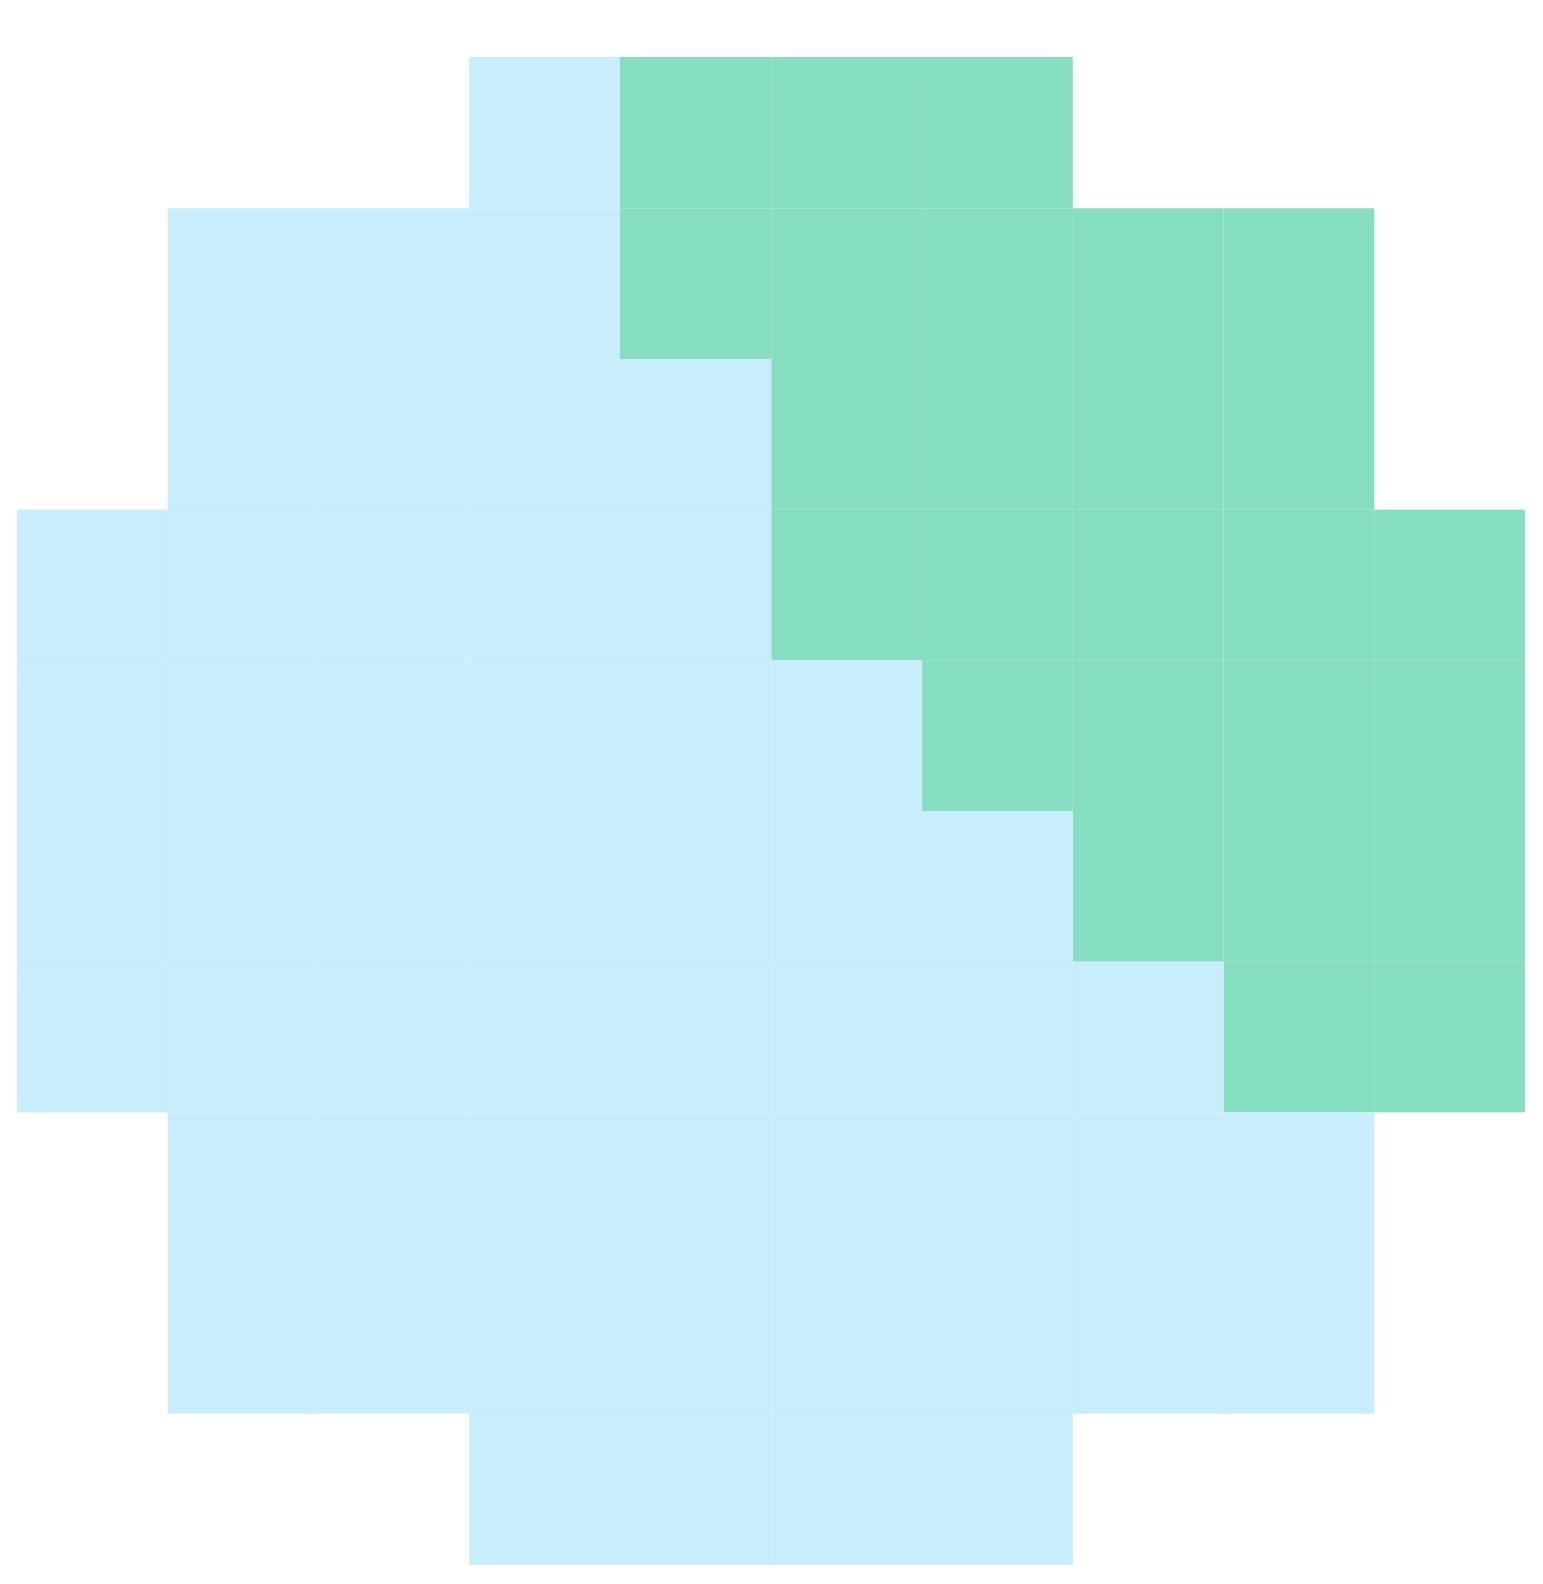
\includegraphics[scale=0.57]{media/2-shabaka/1-vor/dem1.png}
\label{fig:vor1}}
\subfigure[]{%
		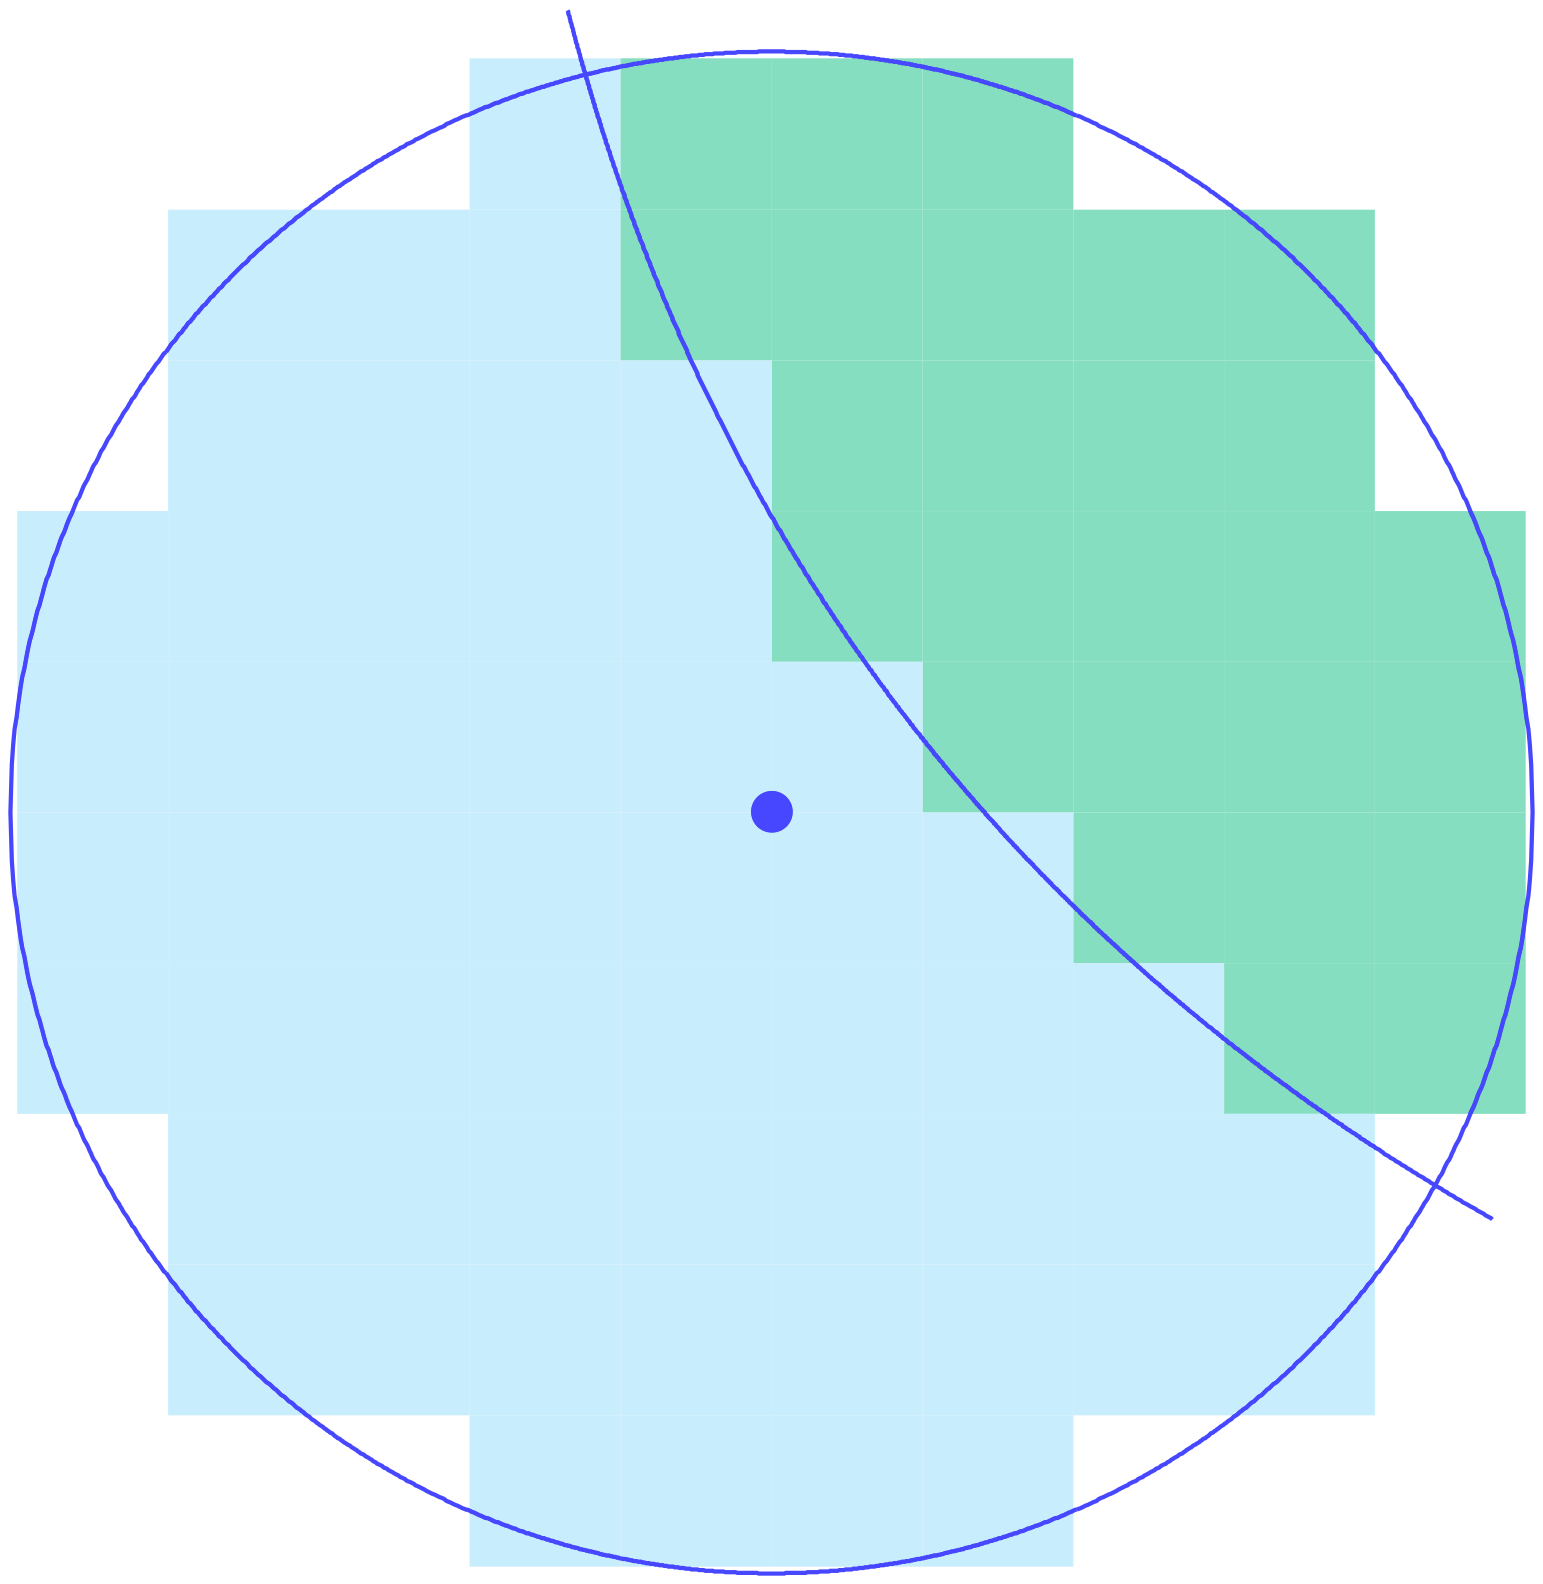
\includegraphics[scale=0.57]{media/2-shabaka/1-vor/dem2.png}
\label{fig:vor2}}
\subfigure[]{%
		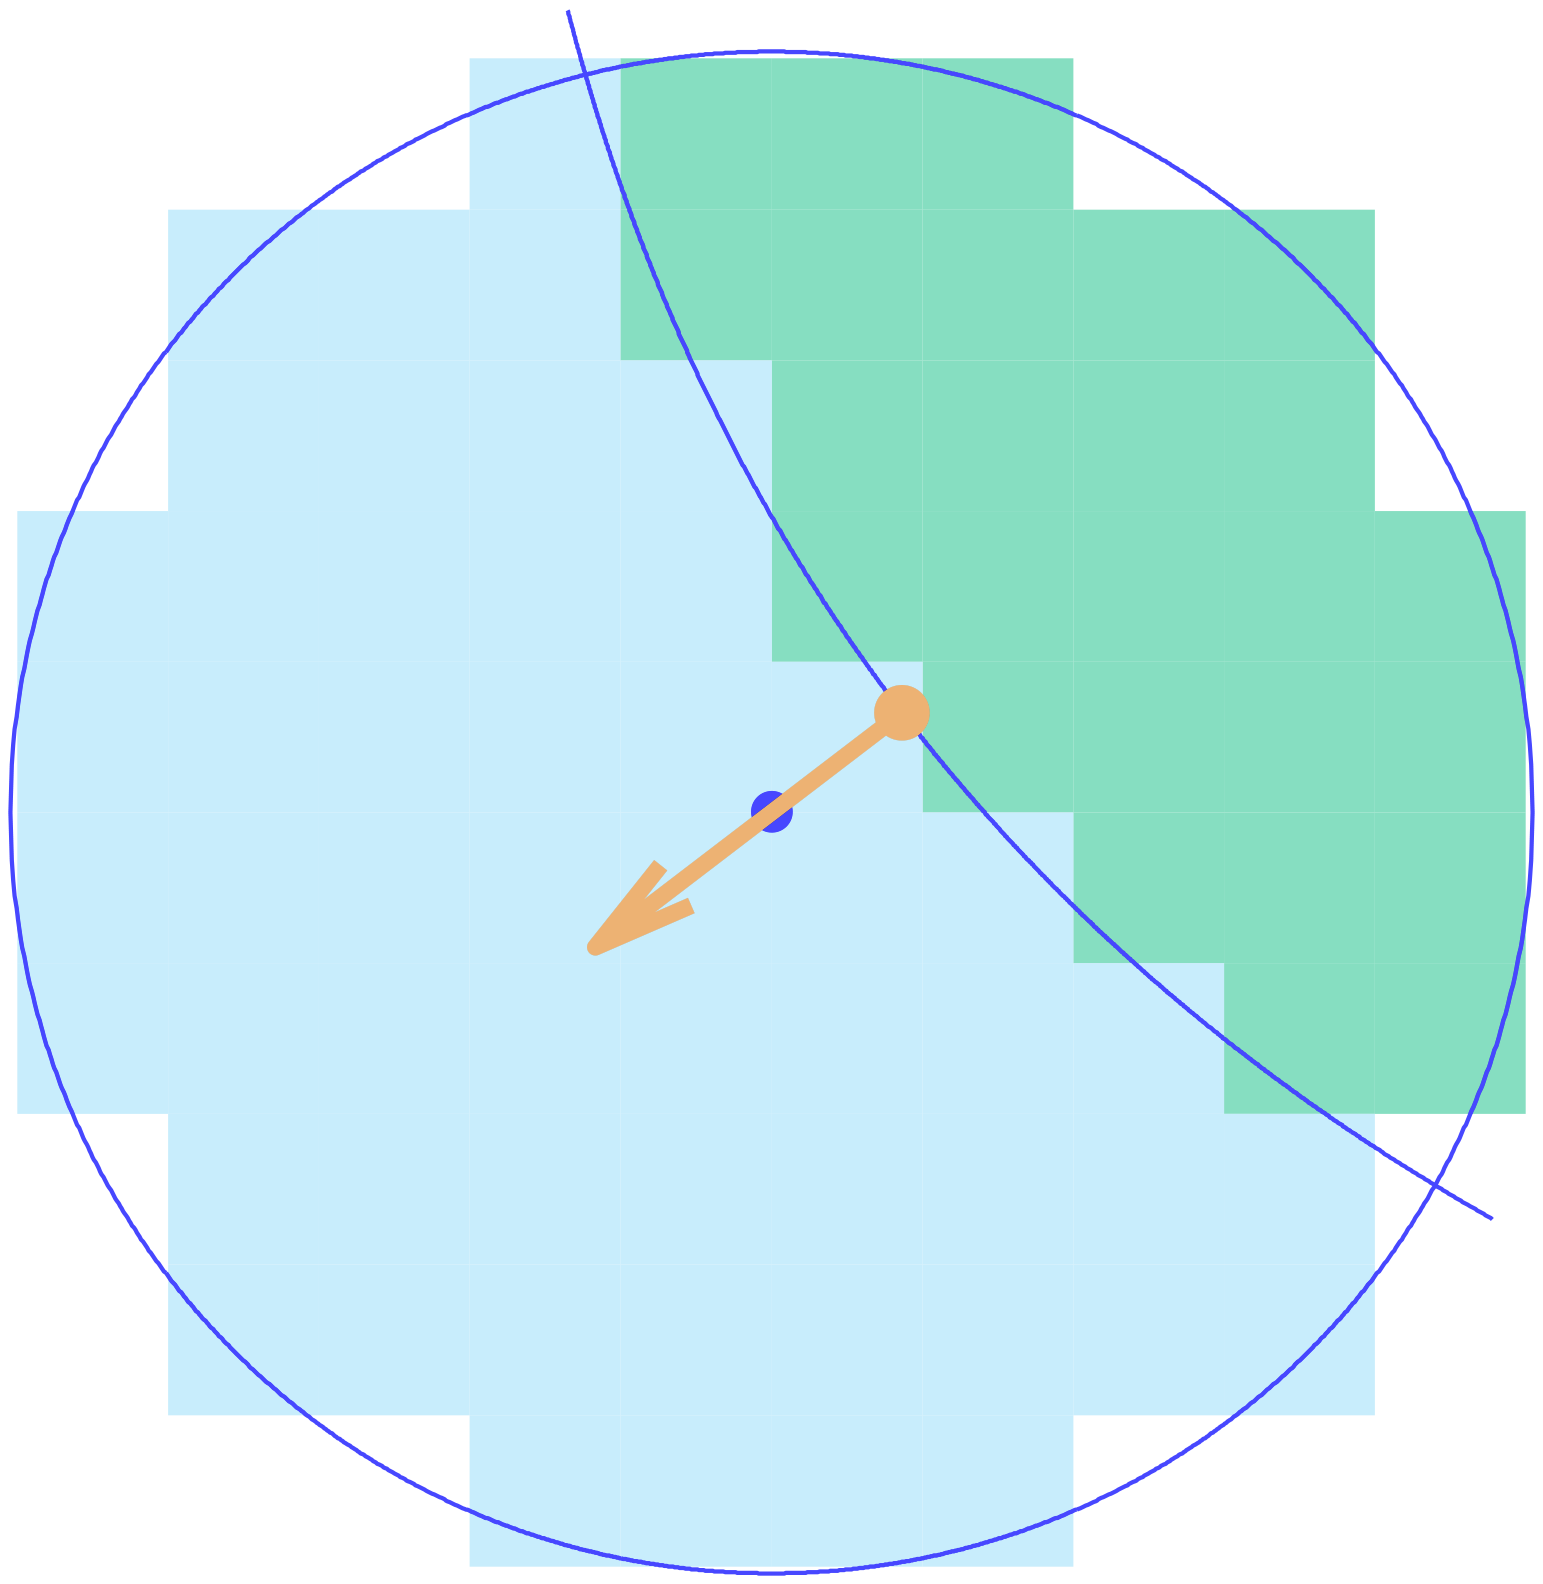
\includegraphics[scale=0.57]{media/2-shabaka/1-vor/dem3.png}
\label{fig:vor3}}
\subfigure[]{%
		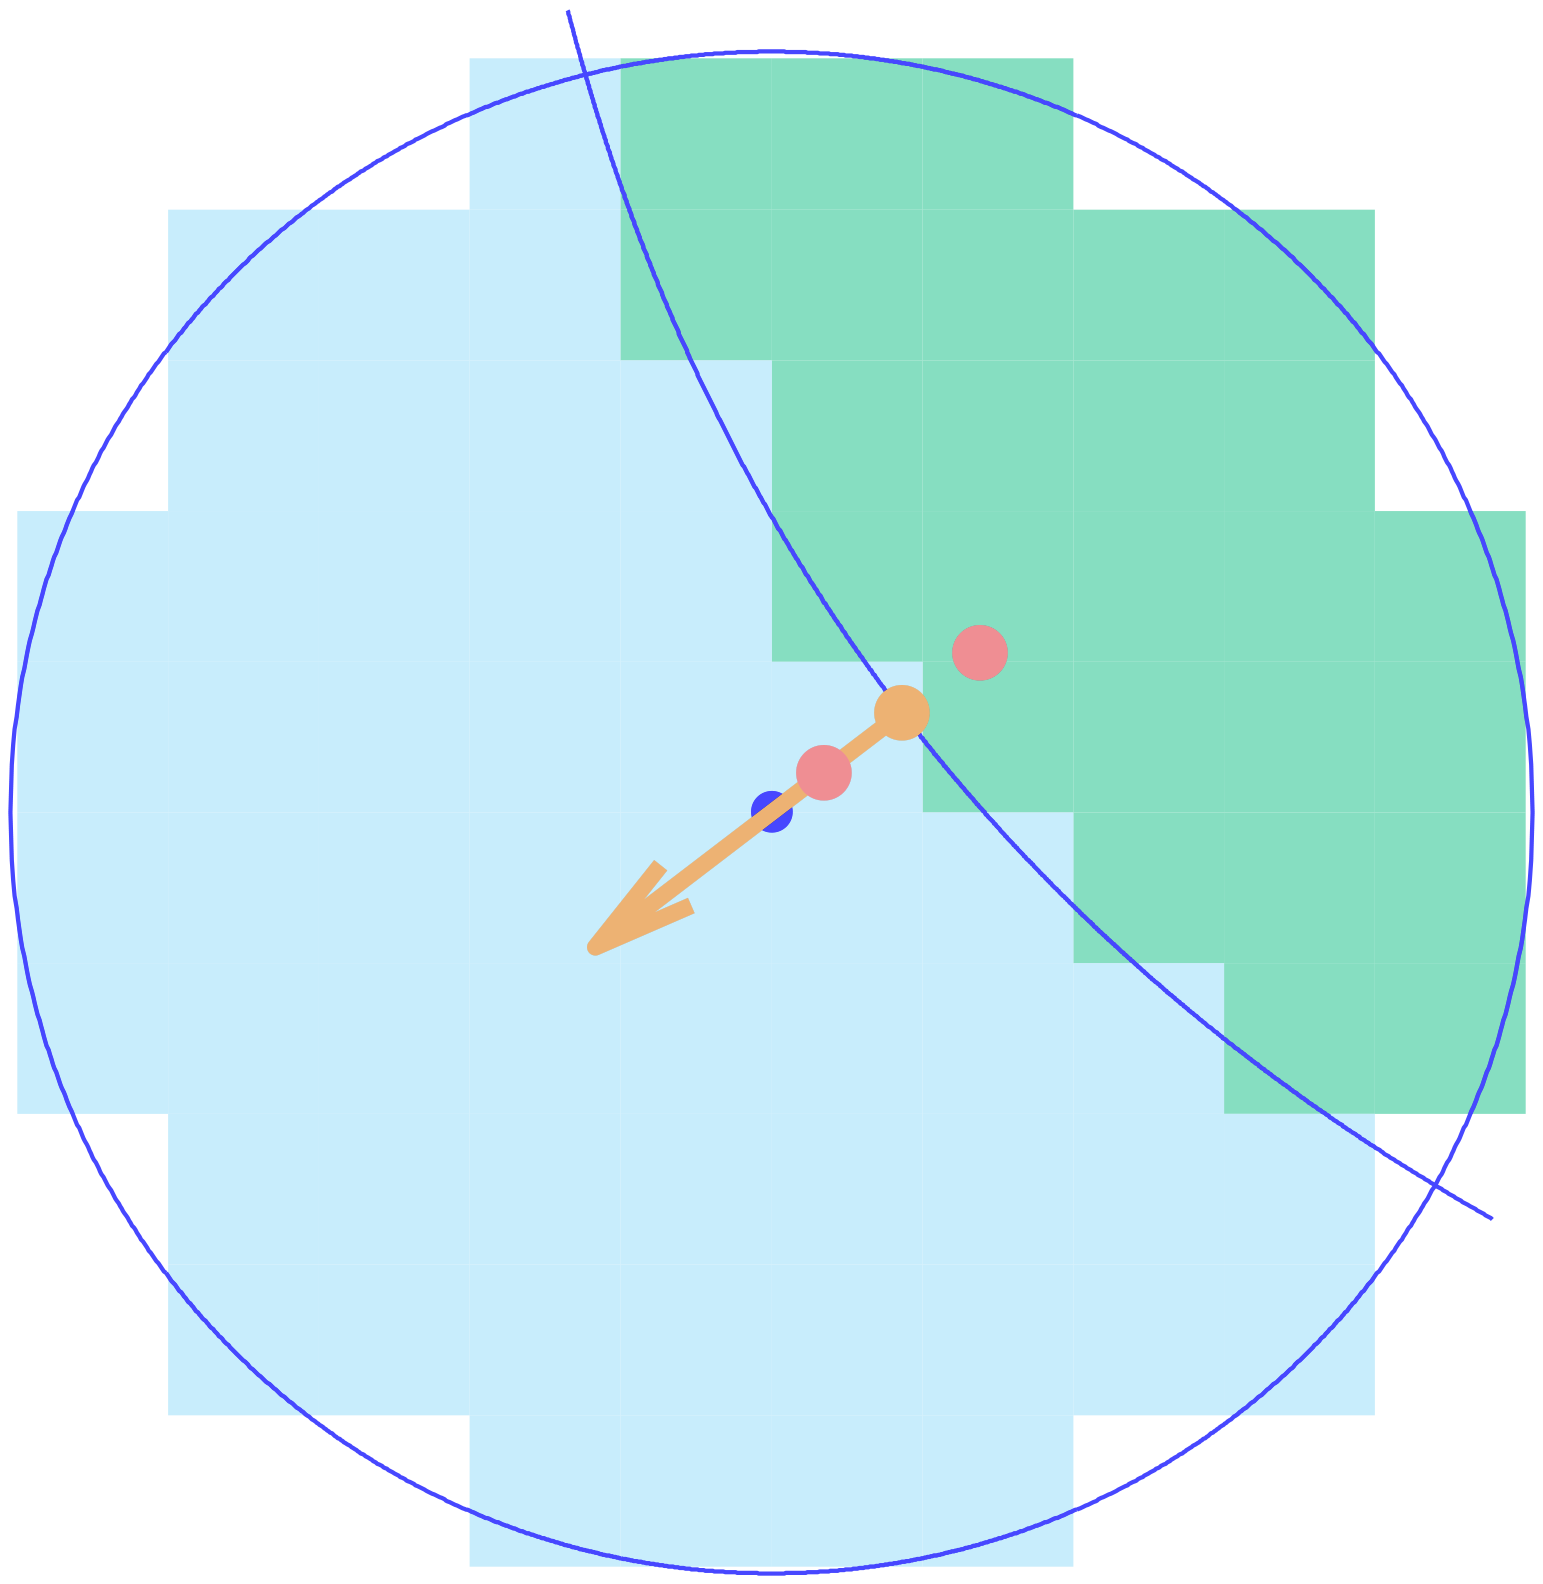
\includegraphics[scale=0.57]{media/2-shabaka/1-vor/dem4.png}
\label{fig:vor4}}
%
\caption{(a) Sampling window of segmented image, (b) interface approximation, (c) point/normal placement, and d) Voronoi site placement. Green voxels belong to the material of interest \textit{m} and blue voxels are void.}
\label{fig:vor}
\end{figure}

\begin{sidewaysfigure}[htbp!]
\centering
\subfigure[]{%
		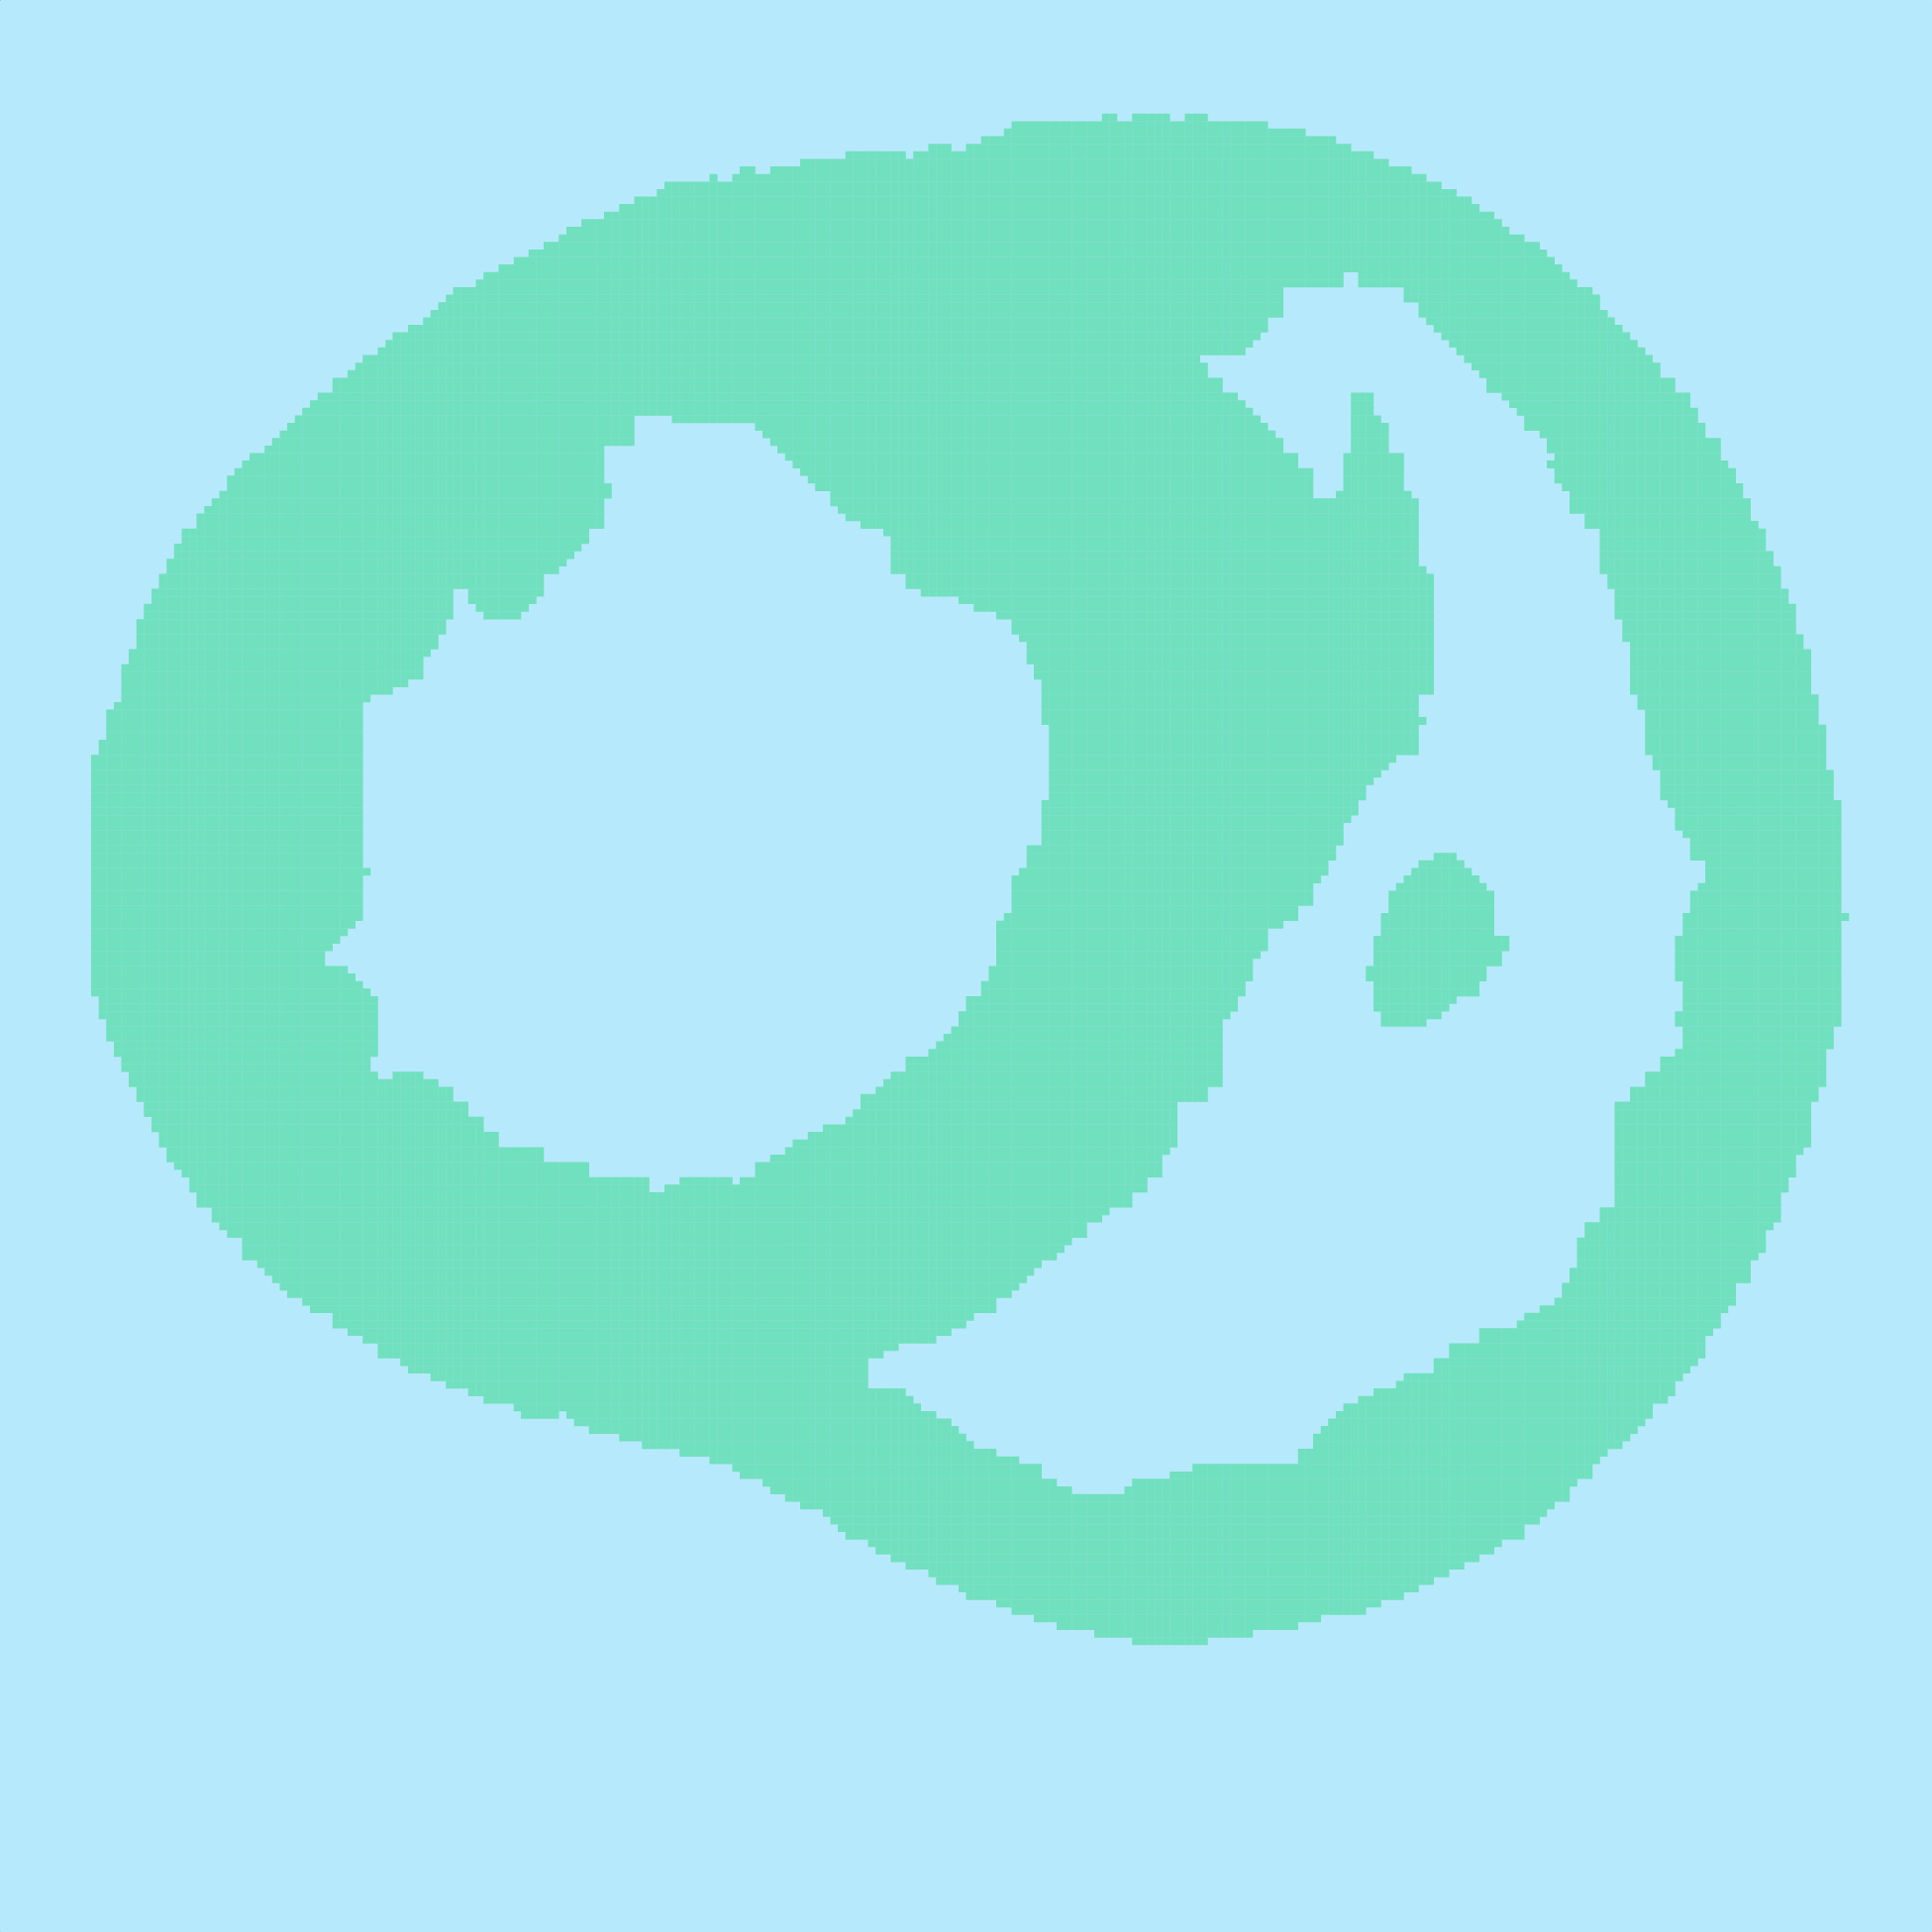
\includegraphics[scale=0.43]{media/vv/a1.png}
\label{fig:d2dvor1}}
\subfigure[]{%
		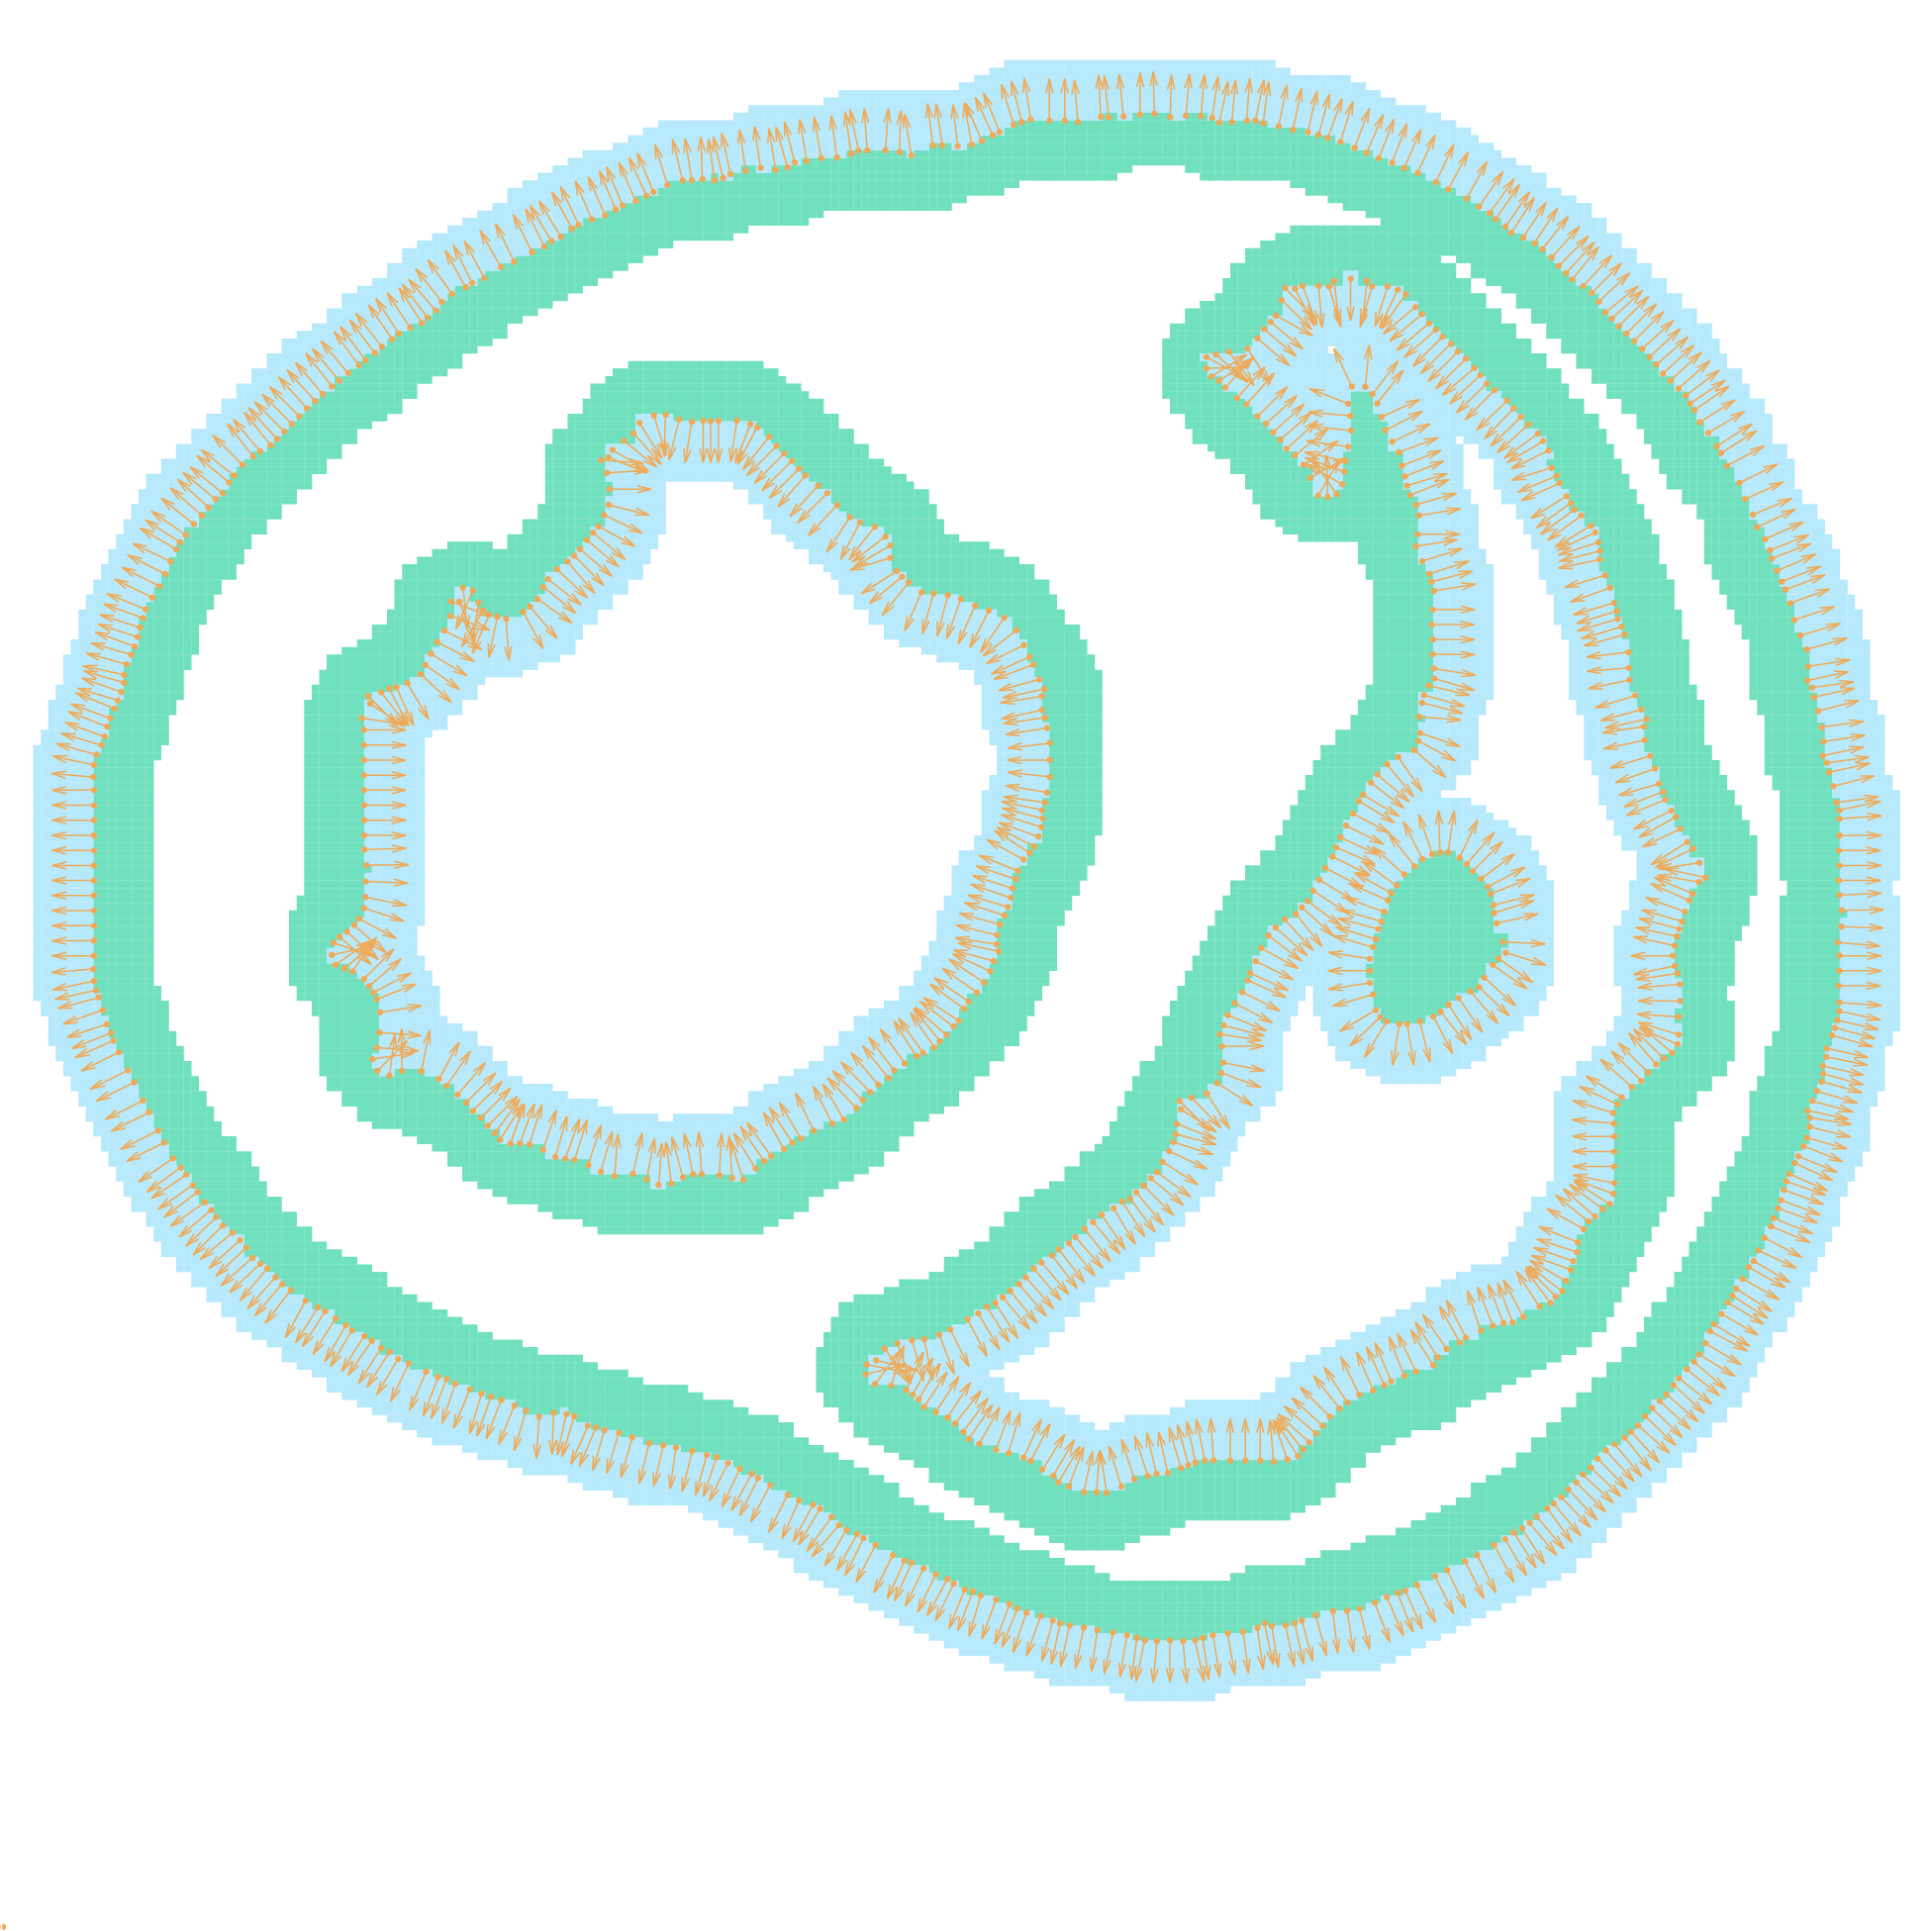
\includegraphics[scale=0.43]{media/vv/a2.png}
\label{fig:d2dvor2}}
\subfigure[]{%
		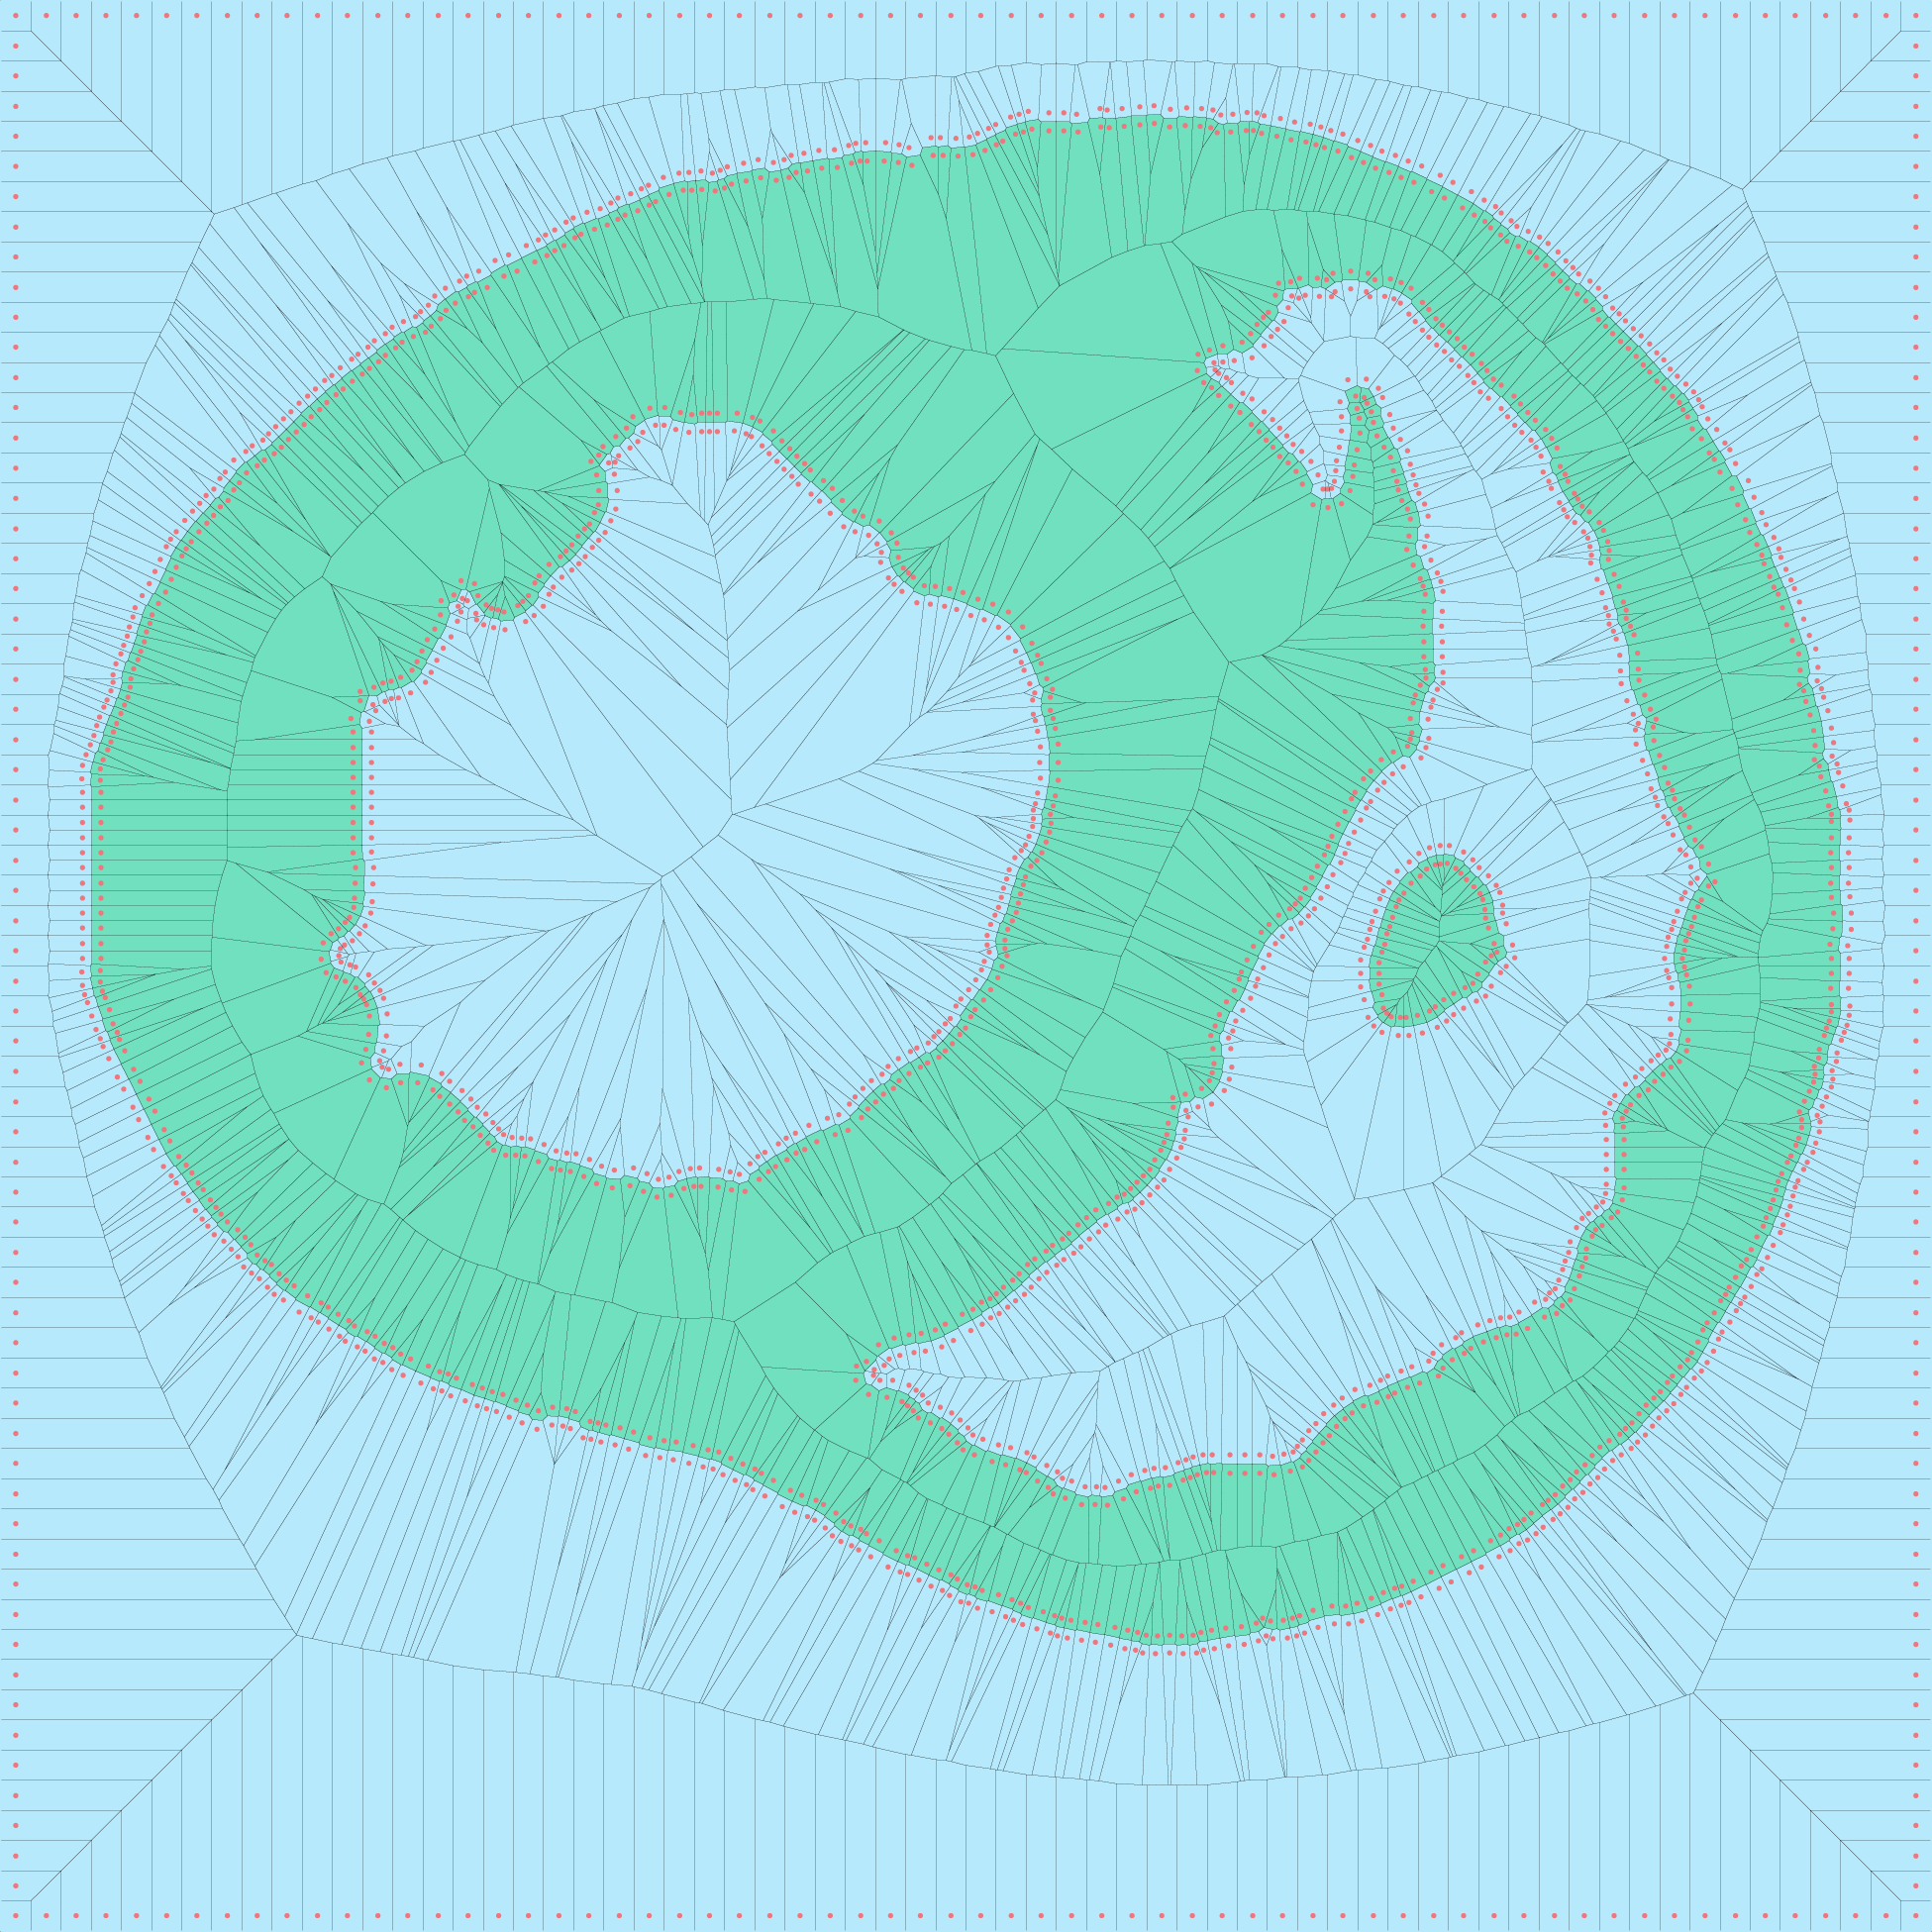
\includegraphics[scale=0.43]{media/vv/a3.png}
\label{fig:d2dvor3}}
%\subfigure[]{%
%		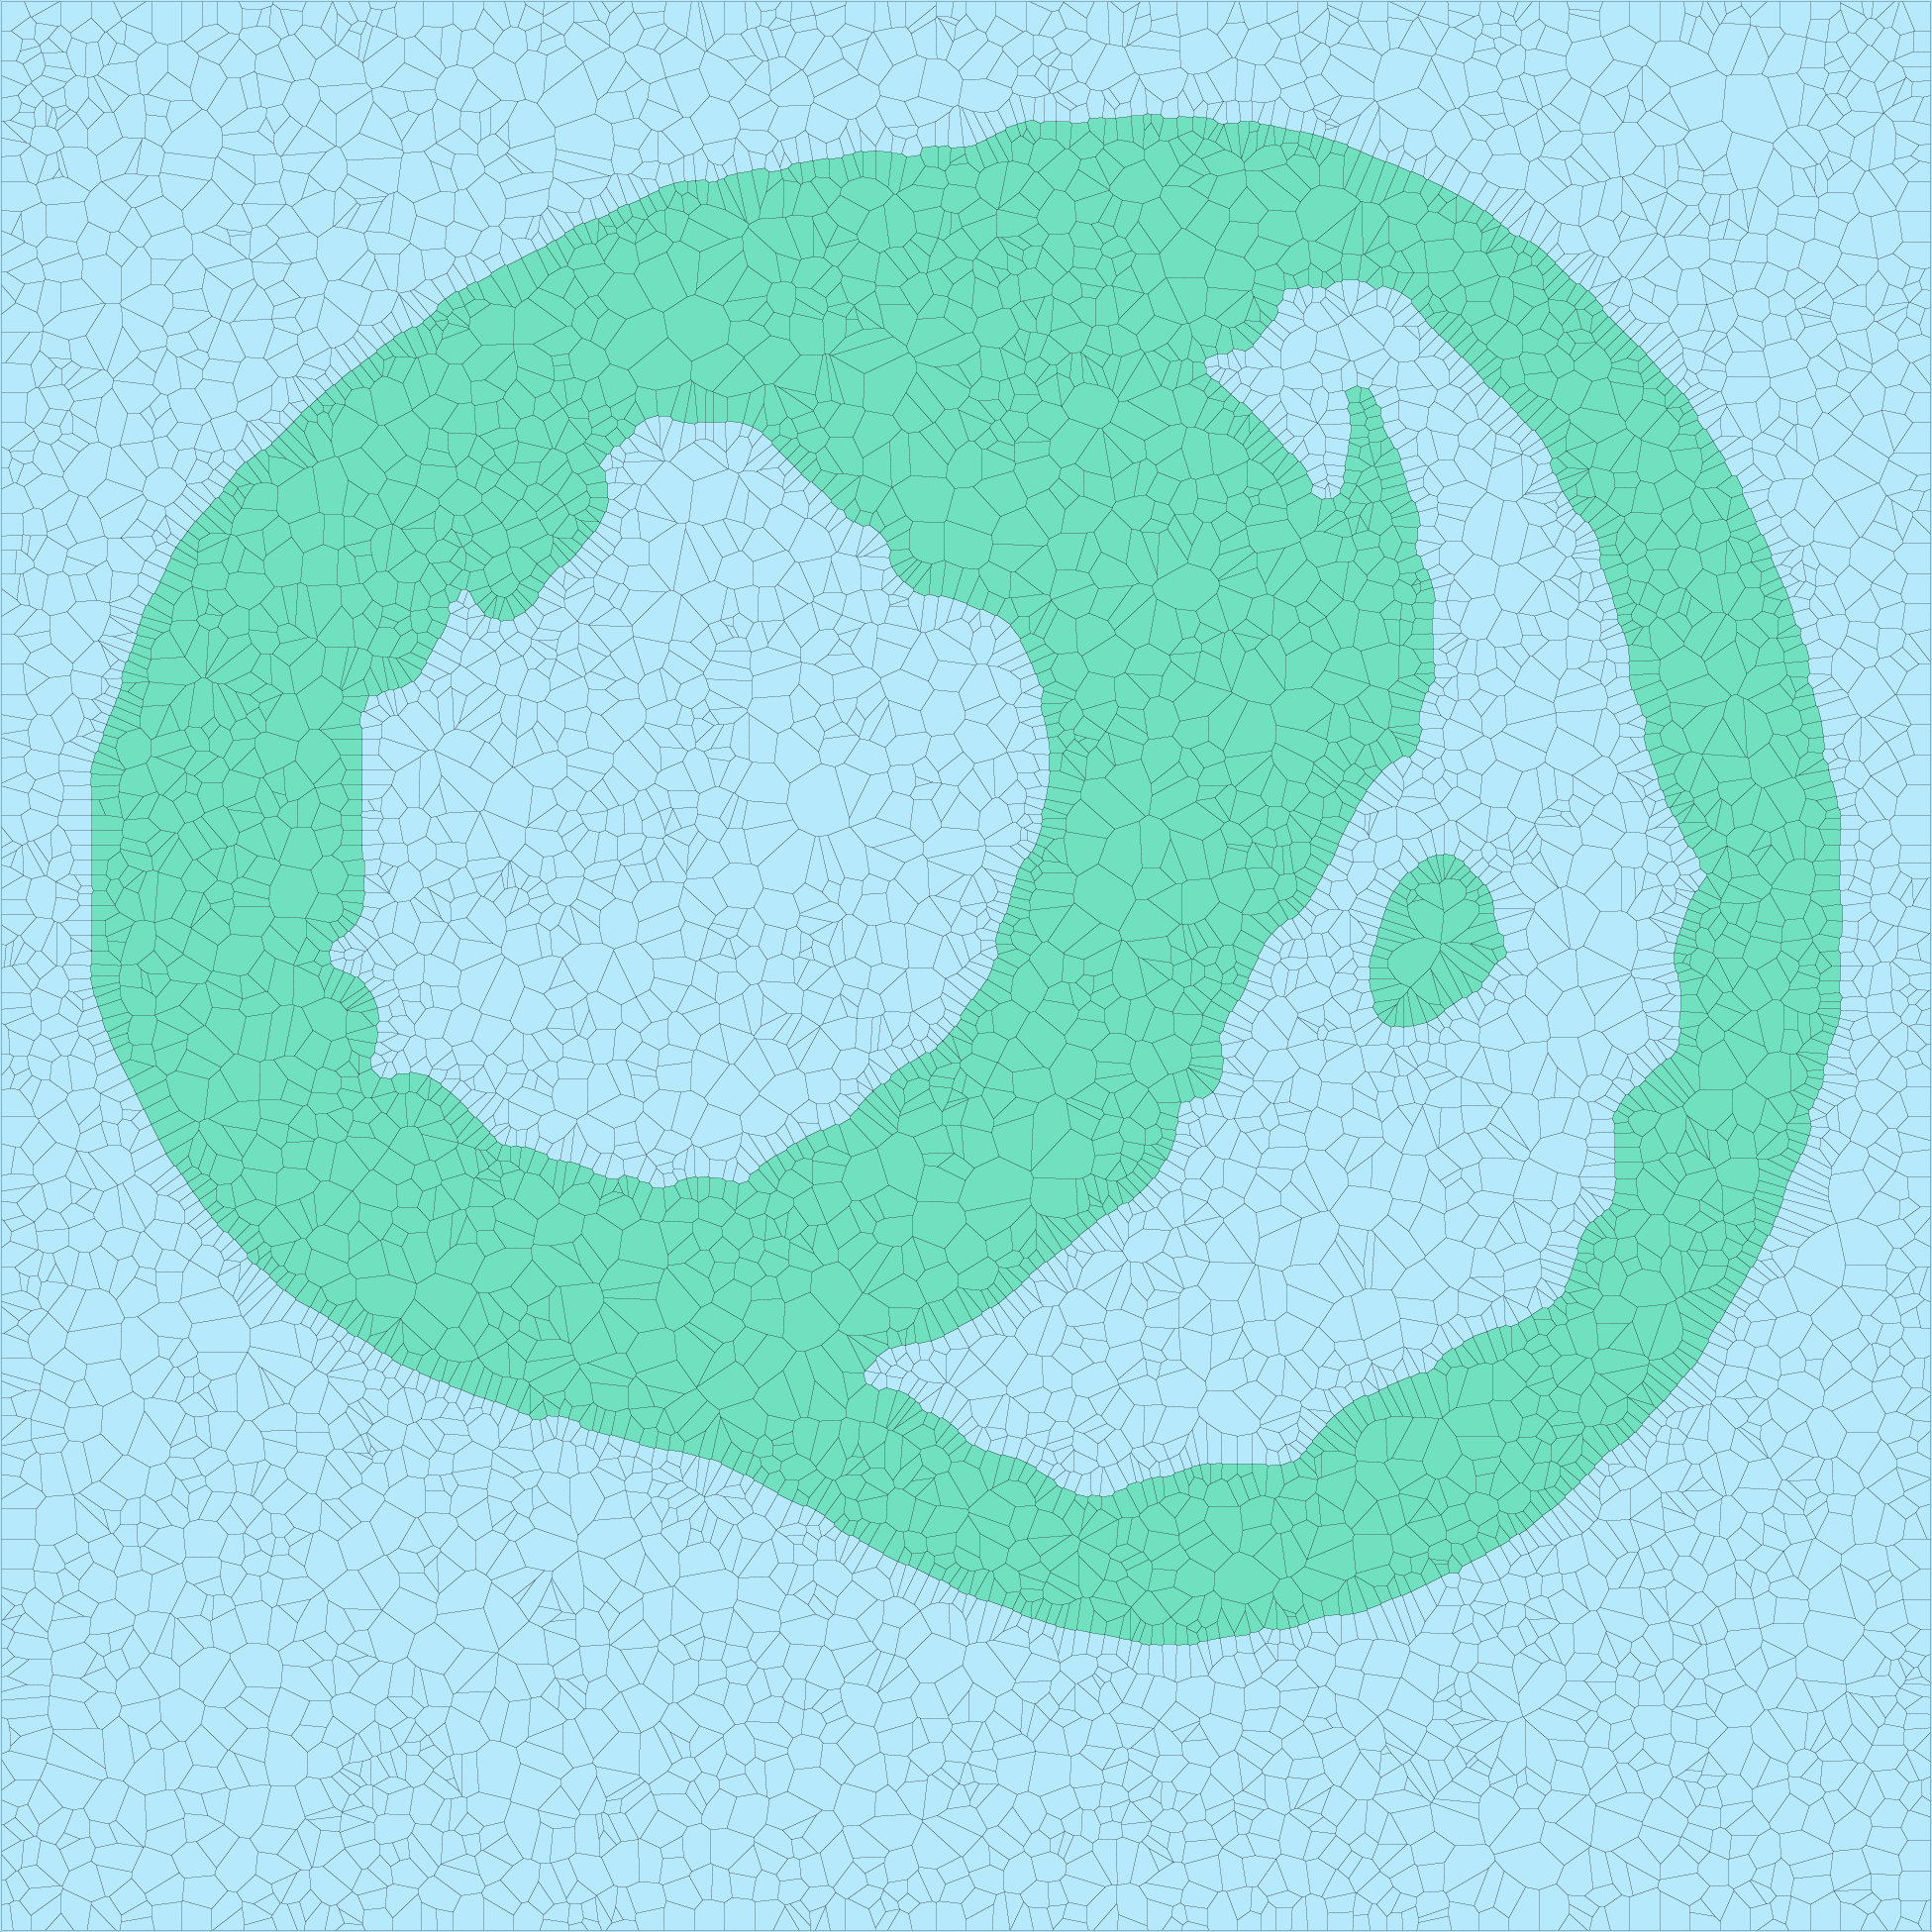
\includegraphics[scale=0.4]{media/vv/a4.png}
%\label{fig:d2dvor4}}
%
\caption{(a) Segmented image of 2D slice of \textit{ex vivo} canine heart, (b) resulting point cloud, and (c) Voronoi site placement and subsequent Voronoi partitioning and surface extraction}
\label{fig:d2dvor}
\end{sidewaysfigure}

\subsubsection{Window Selection}

Define the set of all voxels in a segmented image as $\mathcal{I}$. The segmented image  $\mathcal{I}$ is sampled with overlapping windows, each of which is a voxelized sphere with voxel radius $R_{\mathcal{W}}$. The sampling distance between adjacent windows is $d_{\mathcal{W}}$. The set of voxels in a particular window is defined as $\mathcal{W}$, and the number of voxels in that window is $n_{\mathcal{W}}$. Define the set of voxels in $\mathcal{W}$ that belong to the material of interest $m$ to be $\mathcal{M}$, and the number of voxels in $\mathcal{M}$ to be $n_{\mathcal{M}}$. A window $\mathcal{W}$ is deemed acceptable if it satisfies a threshold requirement. Define $k_{\mathcal{M}}$ as the ratio of voxels in $\mathcal{M}$ to the voxels in $\mathcal{W}$, i.e., $k_{\mathcal{M}} = n_{\mathcal{M}}/n_{\mathcal{W}}$. For a threshold value $\overline{k}_{\mathcal{M}}$, the window is discarded if $k_{\mathcal{M}} > \overline{k}_{\mathcal{M}}$ or $k_{\mathcal{M}} < 1 - \overline{k}_{\mathcal{M}}$. Thus, further calculations are only performed if there are enough voxels of both material \textit{m} and of void to justify approximating a material interface. Refer to~\tabref{window} for a list of these variables and their descriptions. 

\begin{table}[htbp!]
 \centering
   \begin{tabular}{|c||c|}
   \hline
   {\textbf{Variable}} & \textbf{Description} \\ \hline \hline
   $\mathcal{I}$ & set of all voxels in a segmented image \\ \hline
   $\mathcal{W}$ & set of all voxels in a window \\ \hline
   $m$ & material of interest \\ \hline
   {$k_{\mathcal{M}}$} & ratio of voxels in $\mathcal{M}$ to voxels in $\mathcal{W}$\\ \hline
   {$\overline{k}_{\mathcal{M}}$ \rule{0mm}{4mm}} & threshold value for $k_{\mathcal{M}}$ \\ \hline 
   $R_{\mathcal{W}}$ & window radius (in voxels) \\ \hline
   $d_{\mathcal{W}}$ & sampling distance between adjacent windows (in voxels) \\ \hline  
\end{tabular}
\caption{List of variables for window selection}
\label{tab:window}
\end{table}

\subsubsection{Interface Approximation}

For a particular window $\mathcal{W}$, we seek to approximate the interface between voxels belonging to $\mathcal{M}$ and voxels belonging to $\mathcal{W} \setminus \mathcal{M}$ by a surface $\mathcal{S}$. Assuming $\mathcal{W}$ has been deemed acceptable, an approximating sphere $\mathcal{D}$ of radius $R$ is defined, such that the center and volume of this sphere equal the center and volume of the window $\mathcal{W}$, respectively.

Define $\Omega_p$ as the physical space covered by the voxels belonging to $\mathcal{M}$. Define $\Omega$ as the physical space covered by an approximating lens to $\Omega_p$, determined by the space enclosed by the intersection of $\mathcal{D}$ and $\mathcal{S}$. The surface $\mathcal{S}$ is determined by minimizing the error between geometric properties of $\Omega$ and $\Omega_p$~(see~\figref{figure3}).

\begin{figure}[ht]
\centering
\subfigure[Window $\mathcal{W}$]{%
		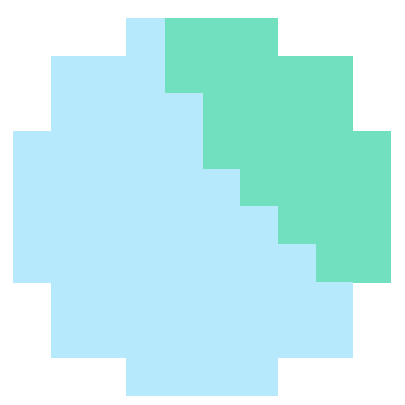
\includegraphics[scale=0.72]{media/om/dem2.pdf}
\label{fig:subfigure2}}
\subfigure[Approximating sphere $\mathcal{D}$]{%
		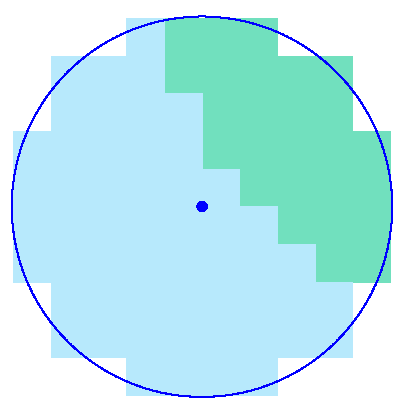
\includegraphics[scale=0.72]{media/om/dem3.pdf}
\label{fig:subfigure3}}

\subfigure[Approximating surface $\mathcal{S}$]{%
		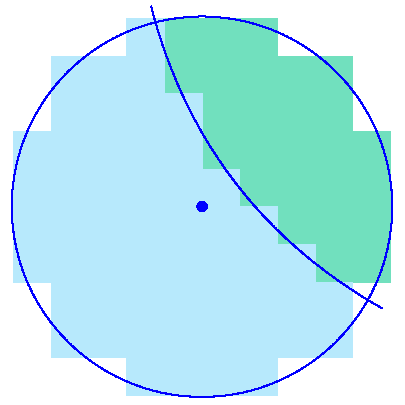
\includegraphics[scale=0.72]{media/om/dem4.pdf}
\label{fig:subfigure4}}
\subfigure[voxelized region $\Omega_p$]{%
		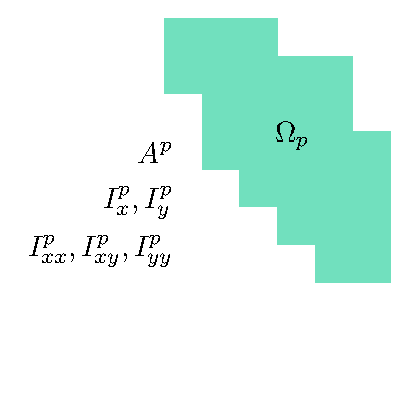
\includegraphics[scale=0.72]{media/om/omp.pdf}
\label{fig:subfigure5}}
\subfigure[Approximating lens $\Omega$]{%
		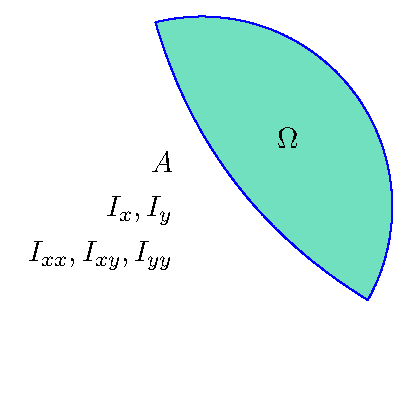
\includegraphics[scale=0.72]{media/om/om.pdf}
\label{fig:subfigure6}}

\caption{Interface approximation demonstrated in 2D}
\label{fig:figure3}
\end{figure}

The open surface $\mathcal{S}$ that approximates the interface takes an assumed form - for these purposes the interface is assumed a plane. If the center of the window is defined as the origin, the planar interface takes the form $x' = d$, where $(x',y',z')$ are the coordinates of a transformed coordinate system and $d$ is the perpendicular distance from the origin to the plane~(see~\figref{quad}).

\begin{figure}[ht!]
	\centering
		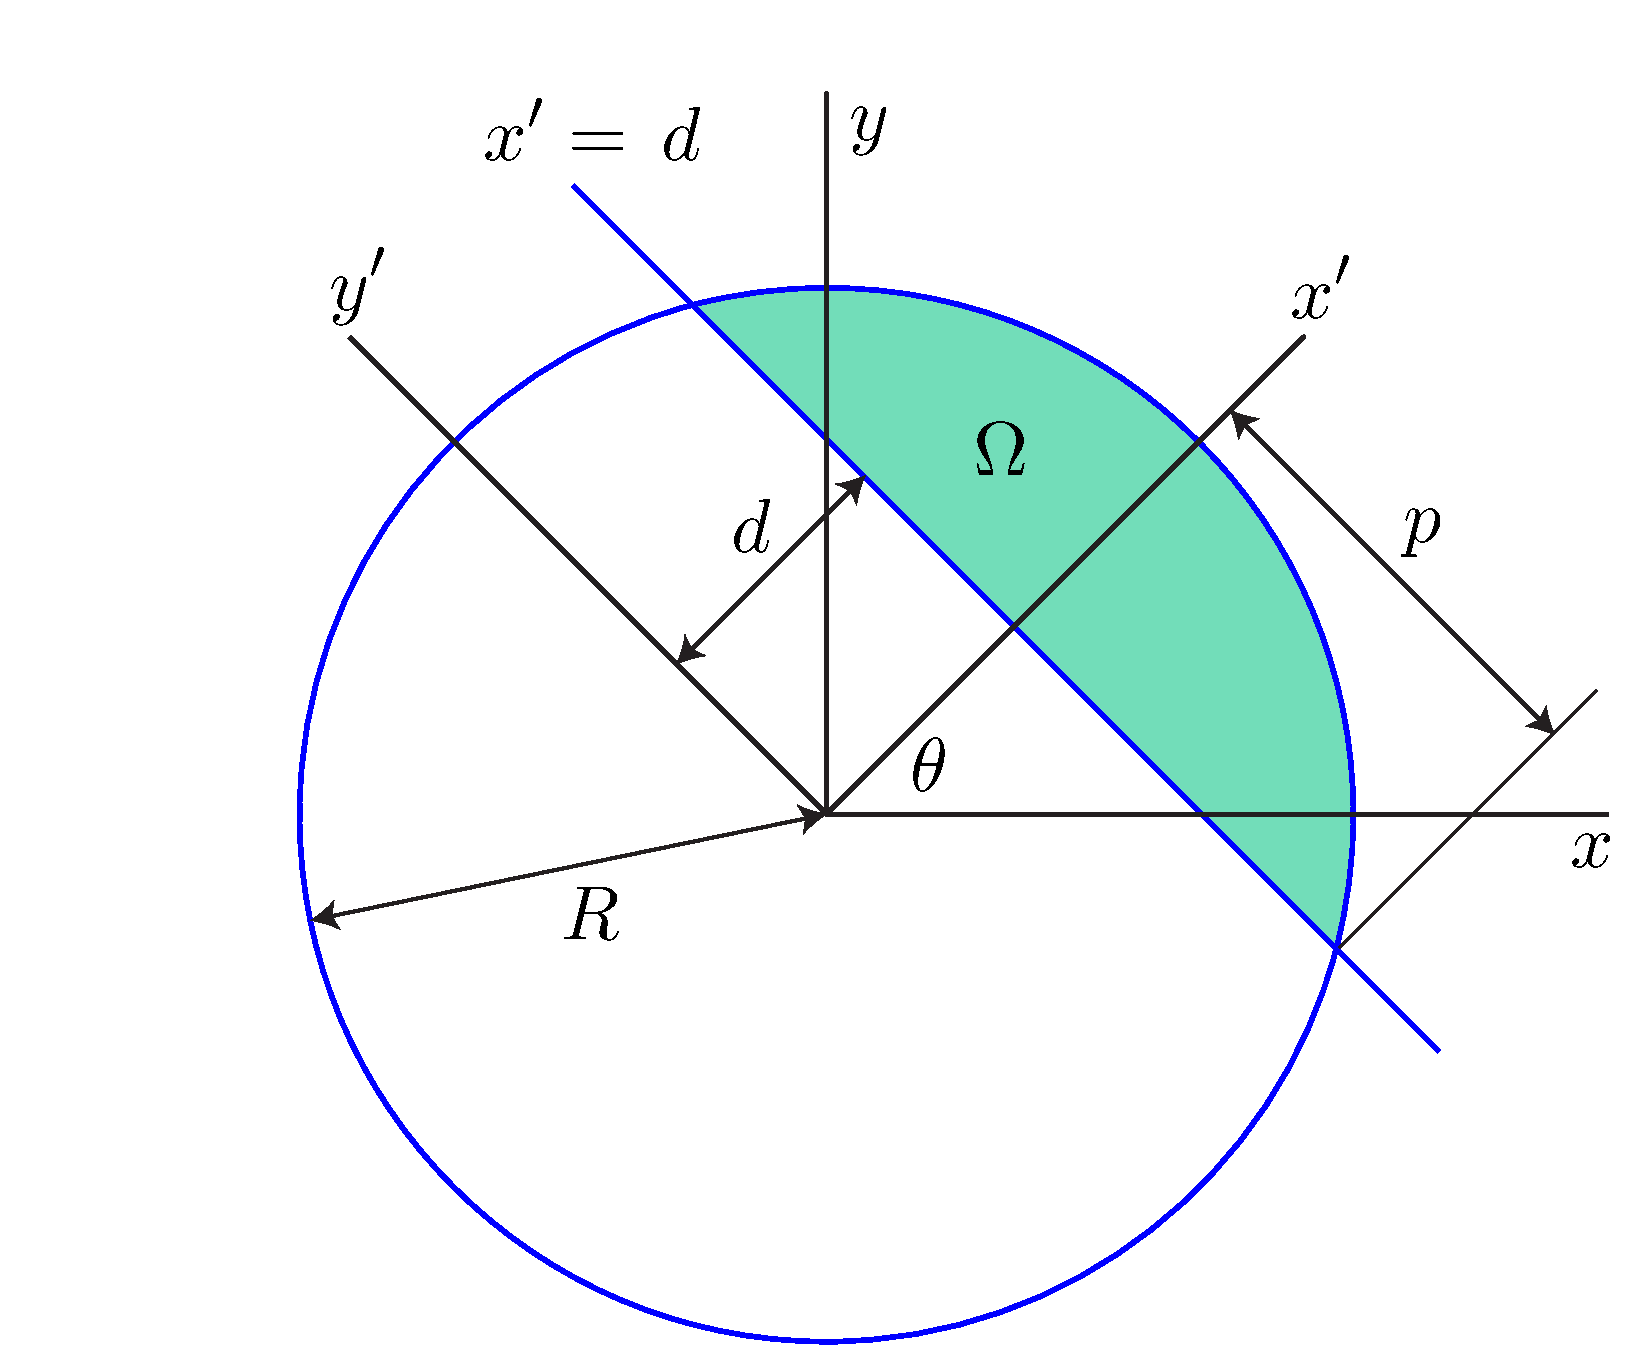
\includegraphics[scale=0.3]{media/om/window.pdf}
	\caption{Plane interface approximation demonstrated in 2D}
	\label{fig:quad}
\end{figure}

Define the following moments of volume for $\Omega_p$:
\begin{alignat}{5}
&{} &&V^p = \int_{\Omega_p}dv &&{} \\
I_{x\phantom{z}}^p &= \int_{\Omega_p}xdv, &&I_{y\phantom{z}}^p = \int_{\Omega_p}ydv, &&I_{z\phantom{z}}^p = \int_{\Omega_p}zdv \\
I^p_{xy} &= \int_{\Omega_p}xydv, &&I^p_{xz} = \int_{\Omega_p}xzdv, &&I^p_{yz} = \int_{\Omega_p}yzdv \\
I^p_{xx} &= \int_{\Omega_p}(y^2 + z^2)dv, \text{\ \ \ \ \ \ }&&I^p_{yy} = \int_{\Omega_p}(x^2 + z^2)dv, \text{\ \ \ \ \ \ }&&I^p_{zz} = \int_{\Omega_p}(x^2 + y^2)dv
\end{alignat}

The zeroth, first, and second moments of volume of $\Omega$ are defined in the same manner, with integrals performed over the domain of $\Omega$ instead.
%\begin{alignat}{5}
%&{} &&V = \int_{\Omega}dv &&{} \\
%I_{x\phantom{z}} &= \int_{\Omega}xdv, &&I_{y\phantom{z}} = \int_{\Omega}ydv, &&I_{z\phantom{z}} = \int_{\Omega}zdv \\
%I_{xy} &= \int_{\Omega}xydv, &&I_{xz} = \int_{\Omega}xzdv, &&I_{yz} = \int_{\Omega}yzdv \\
%I_{xx} &= \int_{\Omega}(y^2 + z^2)dv, \text{\ \ \ \ \ \ }&&I_{yy} = \int_{\Omega}(x^2 + z^2)dv, \text{\ \ \ \ \ \ }&&I_{zz} = \int_{\Omega}(x^2 + y^2)dv
%\end{alignat}
%For the purposes of computing an error functional, define the following quantities:
%\begin{alignat}{3}
%f^p &= V^p, \text{\ \ \ \ \ }&&f(d,\psi,\theta) = V \\
%\bm{g}^p &= \left[\begin{array} {ccc} {I_x^p} \\ {I_y^p} \\ {I_z^p} \end{array} \right], \text{\ \ \ \ \ }&&\bm{g}(d,\psi,\theta) = \left[\begin{array} {ccc} {I_x} \\ {I_y} \\ {I_z} \end{array} \right] \\
%\bm{h}^p &= \left[\begin{array} {ccc} {I_{xx}^p} & {-I_{xy}^p} & {-I_{xz}^p}\\ {-I_{xy}^p} & {I_{yy}^p} & {-I_{yz}^p} \\ -{I_{xz}^p} & {-I_{yz}^p} & {I_{zz}^p} \end{array} \right],\text{\ \ \ \ \ \ \ }&&\bm{h}(d,\psi,\theta) = \left[\begin{array} {ccc} {I_{xx}} & {-I_{xy}} & {-I_{xz}}\\ {-I_{xy}} & {I_{yy}} & {-I_{yz}} \\ -{I_{xz}} & {-I_{yz}} & {I_{zz}} \end{array} \right]
%\end{alignat}

Define the relative errors as:
\begin{align}
e_0(d,\psi,\theta) &=  \sqrt{\frac{(f - f^p)^2}{(f^p)^2}} \\
e_1(d,\psi,\theta) &=  \sqrt{\frac{(g_i - g_i^p)(g_i - g_i^p)}{g_j^{p}g_j^{p}}} \\
e_2(d,\psi,\theta) &=  \sqrt{\frac{(h_{ij} - h_{ij}^p)(h_{ij} - h_{ij}^p)}{h_{kl}^{p}h_{kl}^{p}}}
\end{align}
Finally, we define the relative error functional as follows:
\begin{align}
\mathcal{F}(d,\psi,\theta) = \beta_0e_0 + \beta_1e_1 + \beta_2e_2
\end{align}
where $e_0$, $e_1$, and $e_2$ are relative errors between the zeroth, first, and second order moments of volume of $\Omega_p$ and $\Omega$, respectively. They are functions of the interface parameters $d$, $\psi$, and $\theta$, where $\psi$ and $\theta$ are the yaw and pitch angles defining the plane. The values $\beta_0$, $\beta_1$, and $\beta_2$ are weighting coefficients, where $\beta_2 = 1 - \beta_0 - \beta_1$, and $\beta_i \in [0, 1]$. We seek the solution to the following unconstrained minimization problem: $\displaystyle \min_{d, \psi, \theta} \mathcal{F}(d,\psi,\theta)$, which can be solved by a variety of well-established techniques.

The moments of volume of $\Omega_p$ are computed based on a straightforward use of voxel dimensions and the parallel axis theorem. The moments of $\Omega$, on the other hand, are computed based on an intricate dependence on $d$, $\psi$, and $\theta$:
\begin{align}
p &= \sqrt{R^2 - d^2} \\
V^* &= 2\pi\left[-\frac{1}{2}dp^2 + \frac{1}{3}R^3 - \frac{1}{3}(R^2 - p^2)^{3/2} \right] \\
I^*_{x'x'} &= \frac{\pi}{30}\left[-15dp^4 + \sqrt{R^2-p^2}\left(12p^4 - 4p^2R^2 - 8R^4\right) + 8R^5 \right] \\
\begin{split}
I^*_{y'y'} &= \frac{\pi}{480}\Big[-160d^3p^2 + 128R^5 - \sqrt{R^2-p^2}\left(128R^4 - 96p^2R^2 - 32p^4\right) - 120dp^4 \Big]
\end{split}
\end{align}
\begin{align}
V &=  \begin{cases}
      V^*, & \text{if}\ d \geq 0 \\
      V^* + \frac{4\pi}{3}\left(R^2-p^2\right)^{3/2}, & \text{otherwise}
    \end{cases} \\
I_{x'} &= \frac{\pi}{4}\left[2p^2(R^2-d^2) - p^4 \right]\\
I_{y'} &= I_{z'} = 0 \\
I_{x'y'} &= I_{x'z'} = I_{y'z'} = 0 \\
I_{x'x'} &=  \begin{cases}
      I^*_{x'x'}, & \text{if}\ d \geq 0 \\
       I^*_{x'x'} + \frac{4\pi}{15}(R^2-p^2)^{3/2}(3p^2+2R^2), & \text{otherwise}
    \end{cases} \\
I_{y'y'} &=  \begin{cases}
     I^*_{y'y'}, & \text{if}\ d \geq 0 \\
     I^*_{y'y'} + \frac{2\pi}{15}(R^2-p^2)^{3/2}(p^2+4R^2), & \text{otherwise}
    \end{cases} \\
I_{z'z'} &= I_{y'y'}
\end{align}
Unsurprisingly, certain moments of volume exhibit symmetries in regard to the $y'$ and $z'$ axes. Note that additional terms may exist if $d$ is negative.

The geometric quantities are computed in the transformed coordinate frame and then transformed back to the original desired coordinate frame. This transformation is different for the zeroth, first, and second moments due to the different tensor rank for each of these quantities. Once the moments of $\Omega$ have been transformed to the original coordinate frame, they can be compared to those of $\Omega_p$. The first and second moments are transformed in the following manner (no transformation is required for the zeroth moment of volume):
\begin{align}
\bm{R} &= \left[\begin{array} {ccc} {\cos\psi\cos\theta} & {-\sin\psi} & {\cos\psi\sin\theta}\\ {\sin\psi\cos\theta} & {\cos\psi} & {\sin\psi\sin\theta} \\
{-\sin\theta} & {0} & {\cos\theta}\end{array} \right] \\
\left[\begin{array} {ccc} {I_x} \\ {I_y} \\ {I_z} \end{array} \right] &= \bm{R} \left[\begin{array} {ccc} {I_{x'}} \\ {I_{y'}} \\ {I_{z'}} \end{array} \right]\\
\bm{I}' &= \left[\begin{array} {ccc} {I_{x'x'}} & {-I_{x'y'}} & {-I_{x'z'}}\\ {-I_{x'y'}} & {I_{y'y'}} & {-I_{y'z'}} \\ -{I_{x'z'}} & {-I_{y'z'}} & {I_{z'z'}} \end{array} \right] \\
\bm{I} &= \left[\begin{array} {ccc} {I_{xx}} & {-I_{xy}} & {-I_{xz}}\\ {-I_{xy}} & {I_{yy}} & {-I_{yz}} \\ -{I_{xz}} & {-I_{yz}} & {I_{zz}} \end{array} \right] = \bm{R}\bm{I}'\mathbf{R}^T
\end{align}

With all relevant quantities defined, the \textit{subplex search method}~\cite{rowan} is used to minimize the error functional using an implementation in the package \textit{NLopt}~\cite{nlo}. The method is a \textit{derivative-free} method that is well suited for optimizing objective functions that are noisy or discontinuous. It was selected as the optimization approach due to the existence of square roots in the objective function, and the fact that robustness to a variety of inputs was the highest priority in developing the algorithm. A convergence tolerance $\varepsilon$ is defined such that on successive iterations, $\left| \mathcal{F}_{k+1} - \mathcal{F}_{k}\right| < \varepsilon$, where $k$ is the iteration number. For the specific examples and algorithm parameters to be discussed later in this chapter, convergence is achieved for each interface approximation after typically hundreds of iterations. This large value may be due to the admittedly tight tolerance value for $\varepsilon$ of $10^{-14}$, to nonlinearities or saddle points in the error functional not yet fully understood, or to inefficiencies in the nonlinear optimization tool used. However, because the point cloud generation step generates good results, and the entire process usually completes in less than one minute of wall clock time on a personal computer even for complex geometries, the convergence rate was not further explored as a means for improving the algorithm.

Finally, the solution is only accepted if the error functional is below a specified value $\overline{\mathcal{F}}$, i.e., $\Omega$ approximates $\Omega_p$ to a satisfactory degree. Specifically, we require that once convergence has been satisfied, the criterion $\mathcal{F} < \overline{\mathcal{F}}$ must also be met for the point and normal to be retained. In this way, outlier points for which the error minimization performs poorly are discarded. This typically occurs in regions of high curvature, where a plane does not approximate such an interface well. The point cloud is dense enough that simply discarding these points does not cause any discernible amount of under-sampling of the surface.

The solution to the minimization problem yields the values $d$, $\psi$, and $\theta$ that determine the optimal surface $\mathcal{S}$, from which the interface point and normal are defined. Refer to~\tabref{surface} for a summary of variables used in approximating the interface.

\begin{table}[htbp!]
 \centering
   \begin{tabular}{|c||c|}
   \hline
   {\textbf{Variable}} & {\textbf{Description}} \\ \hline \hline
   $\mathcal{D}$ & approximating sphere to $\mathcal{W}$ \\ \hline
   $\mathcal{S}$ & approximating surface to interface of interest \\ \hline      
   $R$ & radius of $\mathcal{D}$ \\ \hline   
   $\Omega_p$ & physical space covered by voxels belonging to $\mathcal{W}$ \\ \hline
   $\Omega$ & physical space covered by approximating lens of $\Omega_p$ \\ \hline      
   $(x,y,z)$ & axes aligned with image directions, whose origin is at the center of $\mathcal{W}$\\ \hline
   {$(x',y',z')$} & axes $(x,y,z)$ transformed such that $x'$ passes through centroid of $\Omega$ \\ \hline
%   {} & where $x'$ passes through the centroid of $\Omega$ \\ \hline   
   $d$ & perpendicular distance from center of $\mathcal{D}$ to plane $\mathcal{S}$  \\ \hline
   $\psi$ & yaw angle of rotation between $(x,y,z)$ and $(x',y',z')$ axes \\ \hline   
   $\theta$ & pitch angle of rotation between $(x,y,z)$ and $(x',y',z')$ axes \\ \hline
   $V^p$ & volume of $\Omega_p$ \\ \hline
   $I_{x}^p, I_y^p$ & first moments of volume of $\Omega_p$ \\ \hline     
   $I_{xy}^p, I_{xz}^p, I_{yz}^p$ & products of volume of $\Omega_p$ \\ \hline      
   $I_{xx}^p, I_{xy}^p, I_{yy}^p$ & second moments of volume of $\Omega_p$ \\ \hline
   $V$ & volume of $\Omega$ \\ \hline
   $I_{x}, I_y$ & first moments of volume of $\Omega$ \\ \hline
   $I_{xy}, I_{xz}, I_{yz}$ & products of volume of $\Omega$ \\ \hline   
   $I_{xx}, I_{xy}, I_{yy}$ & second moments of volume of $\Omega$ \\ \hline
   $e_0$ & relative error in zeroth moment of volume \\ \hline
   $e_1$ & relative error in first moment of volume \\ \hline
   $e_2$ & relative error in second moment of volume \\ \hline   
   $\beta_0$ & functional weighting coefficient for zeroth moment of volume error \\ \hline
   $\beta_1$ & functional weighting coefficient for first moment of volume error \\ \hline
   $\beta_2$ & functional weighting coefficient for second moment of volume error \\ \hline 
   $\varepsilon$ & convergence tolerance for minimization of functional $\mathcal{F}$ \\ \hline
   $\overline{\mathcal{F}}$ \rule{0mm}{4mm} & largest acceptable value of functional $\mathcal{F}$ \\ \hline        
\end{tabular}
\caption{List of variables for interface approximation}
\label{tab:surface}
\end{table}

\subsubsection{Interface Point and Normal Placement}

Once the parameters $d$, $\psi$, and $\theta$ are selected to fully define the surface that approximates the interface, a point location and outward normal are determined. The outward pointing normal is defined from the transformation of the $x$ axis to the $x'$ axis, i.e., the first column of matrix $\bm{R}$, and thus defined as such: $\bm{n} = -(\cos\psi\cos\theta,\text{\ }\sin\psi\cos\theta,\text{\ }-\sin\theta)$. With the origin at the center of sphere $\mathcal{D}$, the location of the interface normal is then simply $\mathbf{x}_p = -d\bm{n}$.

%%%%%%%%%%%%%%%%%%%%%%%%%%%%%%%%%%%%%%%%%%%%%%%
%%%%%%%%%%%%%%%%%%%%%%%%%%%%%%%%%%%%%%%%%%%%%%%
\subsection{Surface Reconstruction}
\label{Surface Reconstruction}

Surface reconstruction is the process of generating closed, manifold, polygonized surfaces from point clouds. The research found in the literature typically expects a dense, noisy population of points that are generated from laser-based scanners. The proposed algorithm does not in general produce a point cloud as dense as do laser scanners, but a brief review of surface reconstruction techniques is still informative.

Among the most well known surface reconstruction algorithms are the \textit{Power Crust} and \textit{Poisson surface reconstruction} techniques. Amenta \textit{et al.}~\cite{amenta_2001} presented the \textit{Power Crust} algorithm for reconstructing watertight surfaces from unoriented point clouds. It first constructs the \textit{medial axis transform} from the point cloud, which is the set of maximal balls completely contained in the interior of the surface. The algorithm then applies an inverse transform to approximate the medial axis and produce a piecewise-linear surface. The algorithm does not perform well when the point set is not sufficiently dense. Also, it performs quite poorly for point clouds generated from the algorithm described in the previous section. Kazhdan \textit{et al.} presented \textit{Poisson surface reconstruction}~\cite{kazhdan_2008} and subsequently \textit{screened Poisson surface reconstruction}~\cite{kazhdan_2013} for oriented point clouds. They compute an indicator function defined as 1 for points inside the surface and 0 for points outside, whose gradient approximates the vector field defined by the oriented point cloud. This amounts to solving a Poisson problem for an implicit indicator function, followed by application of marching cubes to polygonize the surface. The \textit{screened} approach provides a soft constraint that encourages the reconstructed isosurface to pass through the input points. In practice, the screened approach is significantly more robust than the original approach in generating manifold surfaces from complex point clouds. The technique produces smooth surfaces that exhibit a resiliency to noise, outliers, and under-sampling that is superior to any other technique that has been experimented with.

Many other surface reconstruction approaches exist, including those making use of moving least squares, Delaunay and Voronoi constructions, and variational approaches~\cite{berger}. A novel Voronoi-based approach is presented as an alternative to these approaches that is tuned to address the type of noise and point density from the point cloud generation algorithm from the previous section.

The proposed surface reconstruction technique relies on constructing a \textit{Voronoi diagram}, which for our purposes is a nearest neighbor partitioning of $\mathbb{R}^3$ based on a set of input \textit{Voronoi sites}. The desired output from a Voronoi partition is a mesh - namely, a set of points, edges, facets, and cells (and their connectivities) that discretize space. Define a half-space $D(\bm{p},\bm{q})$ comprising all points $\bm{x}$ as close, or closer, to site $\bm{p}$ than to site $\bm{q}$:
\begin{equation}
D(\bm{p},\bm{q}) = \{\bm{x} \mid d(\bm{p},\bm{x}) \leq d(\bm{q},\bm{x})\}
\end{equation}
where a distance function $d$ must be defined. Although there are instances of more exotic distance functions leading to modified Voronoi approaches, the distance function for standard Voronoi diagrams is simply the Euclidean distance. The \textit{Voronoi cell} $V(\bm{p})$ associated with site $\bm{p}$ is the intersection of all half-spaces involving site $\bm{p}$ and all other sites $\bm{q}$ belong to the set $\mathcal{P}$:
\begin{equation}
V(\bm{p}) = \bigcap \limits_{\bm{q} \in \mathcal{P}, \bm{q} \neq \bm{p}} D(\bm{p},\bm{q})
\end{equation}
A number of important properties exist for Voronoi partitions and their dual \textit{Delaunay tessellations}. For these purposes, though, the most important property is that the surface extracted from a set of Voronoi cells connected by shared facets is watertight and manifold. Several important considerations must be made in constructing a Voronoi partition, including degenerate and near-degenerate cases, the data schema and order of construction of the connected polytopes, and the
performance of the algorithm. Refer to Aurenhammer~\cite{aurenhammer_1991} for a detailed survey of the mathematical and algorithmic approaches to Voronoi diagrams.

The proposed technique involves the following steps, to be described in turn:
\begin{itemize}[noitemsep]
\item Generate Voronoi site set from oriented point cloud and perform Voronoi partition of image
\item Define b-rep as the set of facets that share Voronoi sites with different material types, and perform cleanup on that surface
\item Decimate (coarsen) the surface to a more tractable mesh resolution
\end{itemize}

\subsubsection{Voronoi Site Generation and Voronoi Partitioning}

Given the location of an interface point $\bm{x}_p$ and orientation of its corresponding normal $\bm{n}$, two Voronoi sites are placed on either side of the point along the line of action of the normal, as shown in~\figref{vor4} and~\figref{d2dvor3}. They are separated from the point by a distance $b$, and thus their locations are $\bm{x}_p \pm b \bm{n}$. The two Voronoi sites are assigned material types. For the two-material case considered here, the site corresponding to the position $\bm{x}_p - b\bm{n}$ is inside $\Omega$, and thus is assigned material $m$. The site corresponding to the position $\bm{x}_p + b\bm{n}$ is outside $\Omega$, and thus is assigned a void material. \textit{Voronoi partitioning} is performed using an implementation from \textit{Qhull}~\cite{barber_1996}, that is robust even for near-degenerate Voronoi site locations.

\subsubsection{Surface Extraction and Cleanup}

The b-rep is extracted from the Voronoi partition as the set of facets that share Voronoi sites of differing material types. An additional step is performed, however, to mitigate undesired ``cross-talk'' facets caused by Voronoi partitioning of neighboring site pairs. ``Good facets'' are identified as those b-rep facets whose Voronoi sites belong to a site pair originating from the same point and normal, and ``bad facets'' are those b-rep facets whose Voronoi sites originate from different points in the point cloud. For surfaces with small curvature, the area of good facets significantly outweighs that of the bad facets. Nonetheless, the existence of bad facets causes a stair-stepping feature in the resulting surface that is unacceptable.

The artifact is addressed as follows: ``bad edges'' are identified as those edges that share two bad facets. Networks of connected bad edges are identified, and each network is collapsed to one point (see \figref{cross1}). In the simplest case, for a surface with a small amount of curvature, no bad edges are connected and each is independently collapsed. Any good facet that is connected to a network of bad edges is modified to connect to the new collapsed point. The good facets are triangulated to maintain planarity following the removal of bad facets. This increases the data required to define the surface mesh, but the decimation step described in the next section resolves this issue immediately. The sequence is demonstrated on the full \textit{ex vivo} heart example in~\figref{cross2}.

\begin{sidewaysfigure}[htbp!]
\centering
\subfigure[]{%
		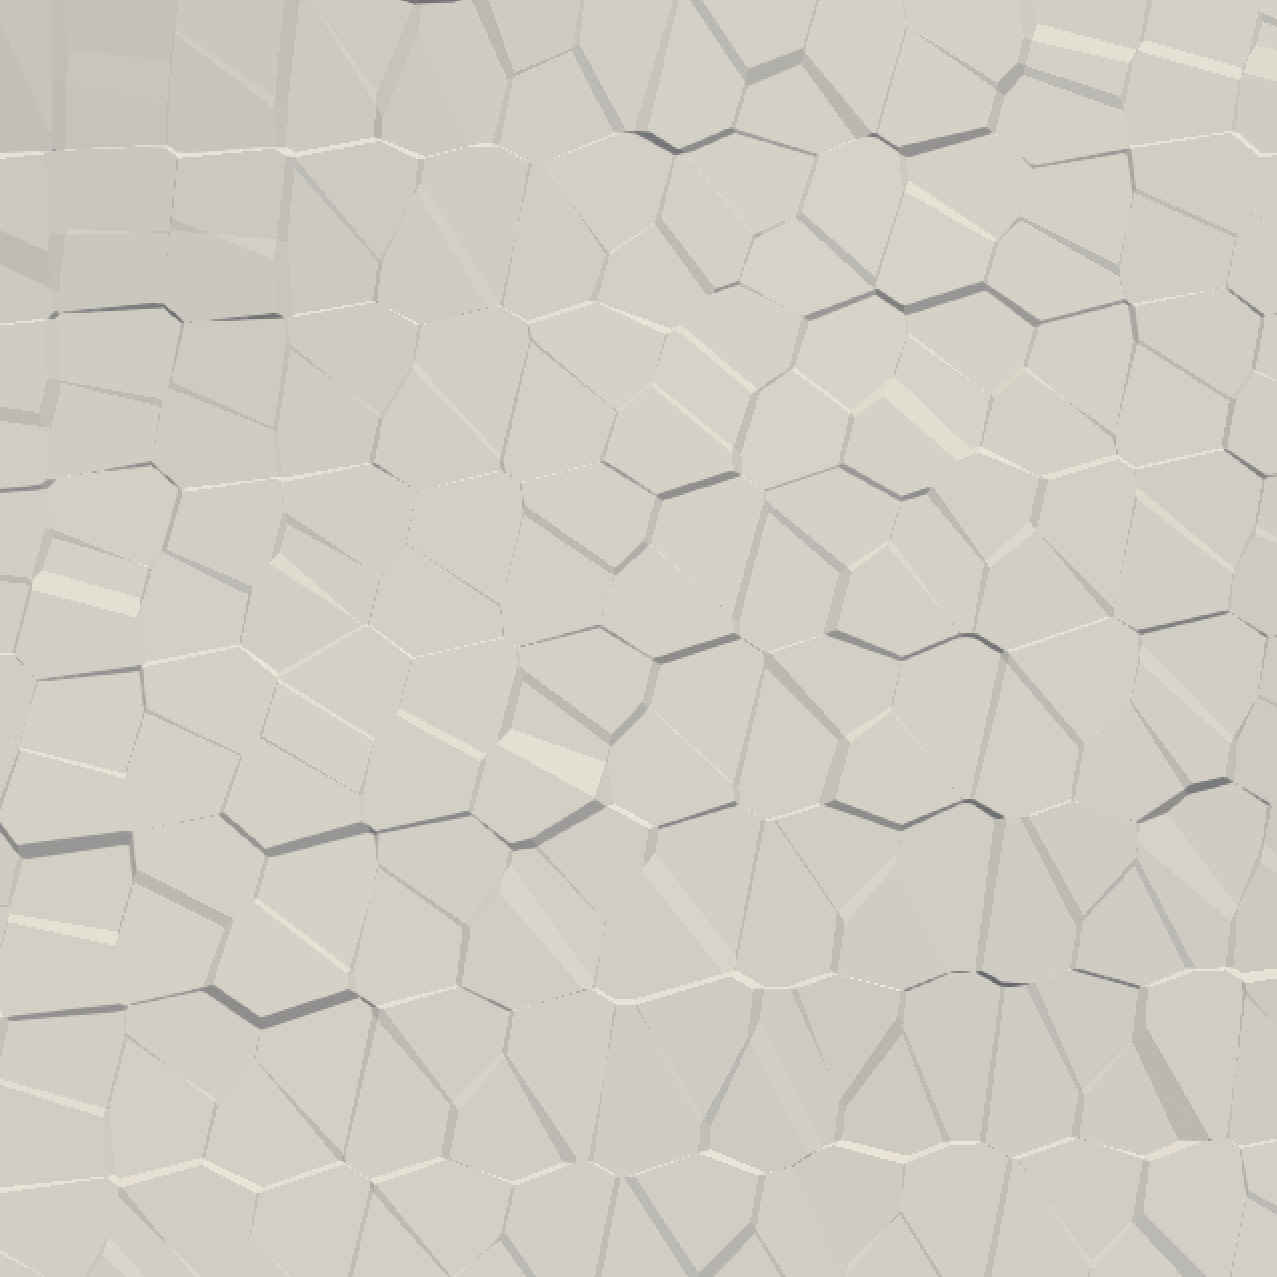
\includegraphics[scale=0.11]{media/2-shabaka/3-clean-zoom/1-init-zoom.png}
\label{fig:cross1-1}}	
\subfigure[]{%
		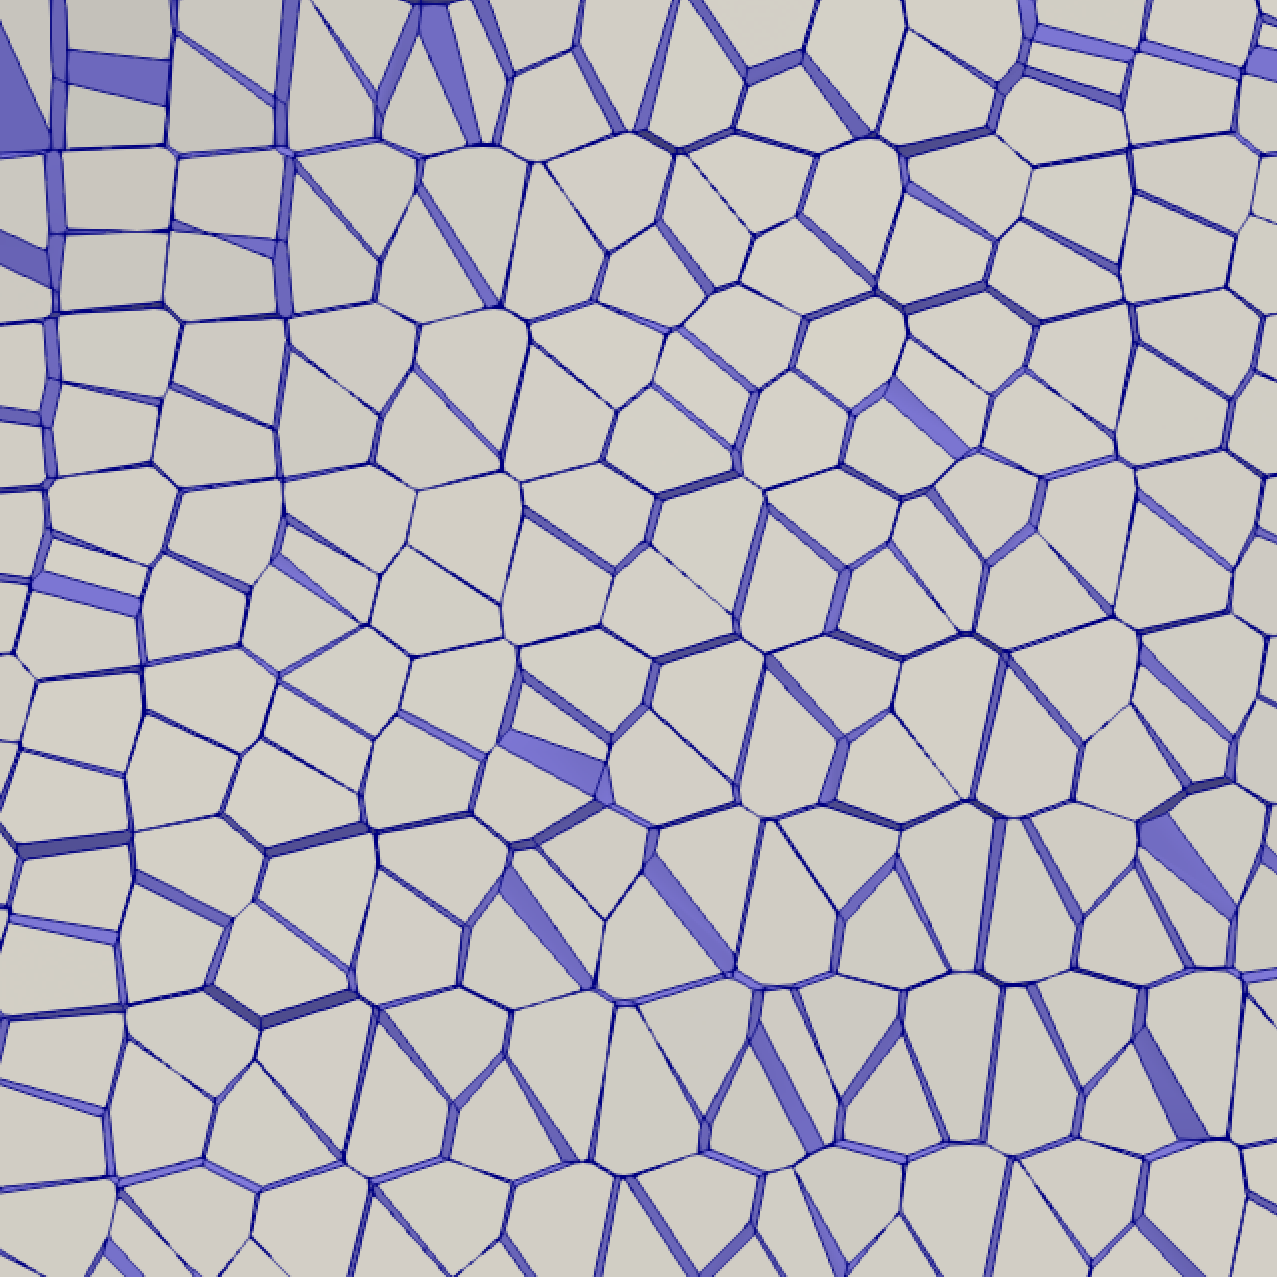
\includegraphics[scale=0.11]{media/2-shabaka/3-clean-zoom/2-badfacets-zoom.png}
\label{fig:cross1-2}}
\subfigure[]{%
		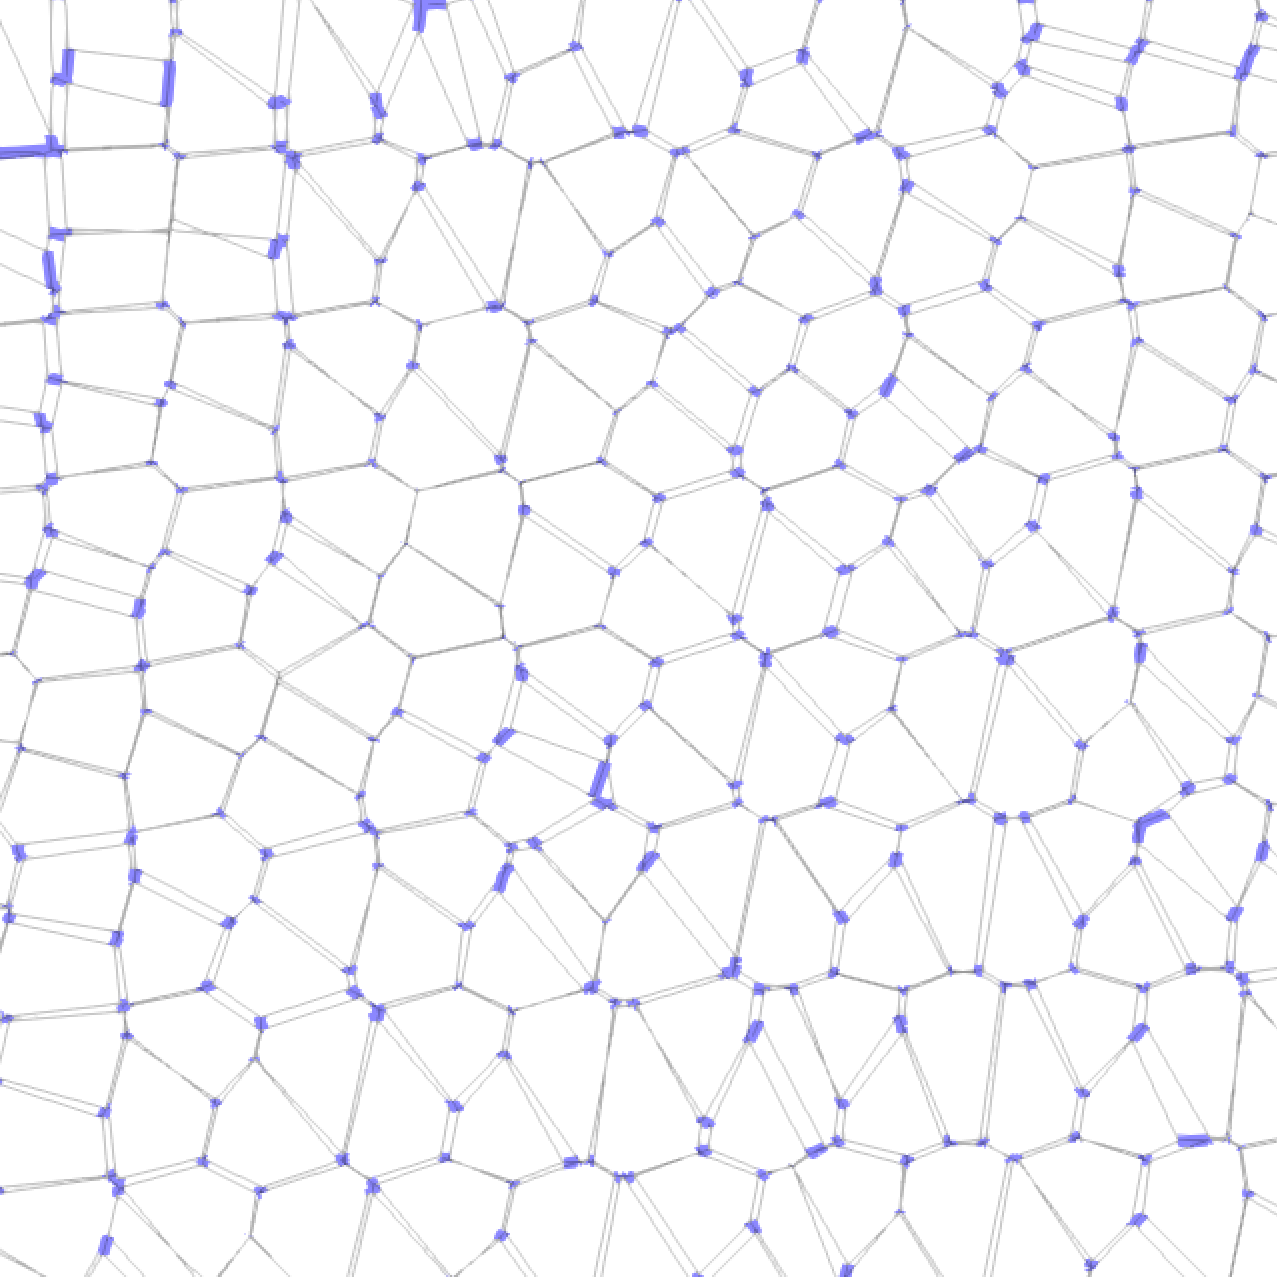
\includegraphics[scale=0.11]{media/2-shabaka/3-clean-zoom/3-badsegs-zoom.png}		
\label{fig:cross1-3}}
\subfigure[]{%
		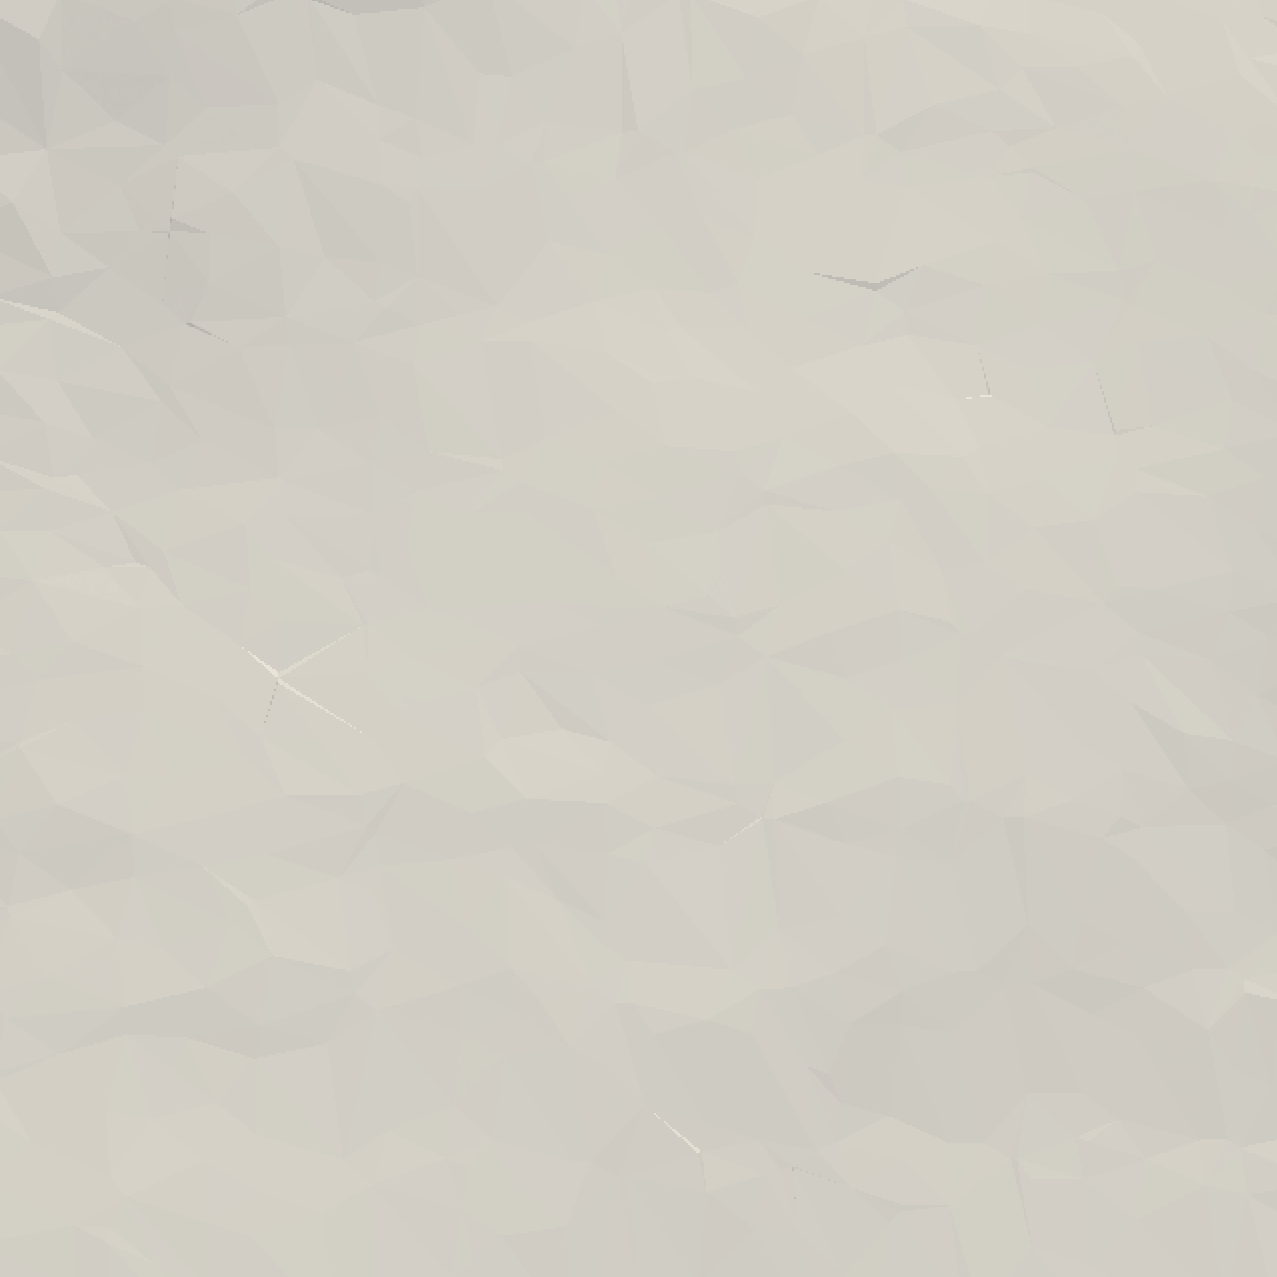
\includegraphics[scale=0.11]{media/2-shabaka/3-clean-zoom/4-fine-zoom.png}
\label{fig:cross1-4}}				
%
\caption{Clean-up of undesirable ``cross-talk'' facets for a surface patch: (a) initial surface following Voronoi-based surface reconstruction, (b) identification of ``cross-talk'' facets, (c) identification of edges to be collapsed, (d) final cleaned surface}
\label{fig:cross1}
\end{sidewaysfigure}

For the vast majority of bad edge networks, the collapse technique results in a smoother surface that remains closed and manifold. For regions of high-curvature, there is a small set of cases in which the clean-up step may cause the surface to become non-manifold. The topology of particular networks of bad edges that cause this phenomenon are identified based on heuristics, and are not collapsed to preserve the manifold property. The current approach thus does not capture regions of high curvature well during the point cloud generation step, and furthermore is unable to alleviate the issue of ``cross-talk'' facets in regions of high curvature. Fortunately, these remaining artifacts are small enough that the ensuing decimation step removes them.

Handling regions of curvature or even sharp corners and edges can certainly be done, though. The technique would involve including additional templates in the interface approximation step that would allow more than two Voronoi sites to be generated for each sampling window. For example, three Voronoi sites can be used to produce an edge, and four sites can be used to produce a corner. This would significantly improve the point cloud approximation of the underlying surface, perhaps to a degree that the collapsing technique described would remove all cross-talk facets with no concern of losing manifoldness.

\begin{sidewaysfigure}[htbp!]
\centering
\subfigure[]{%
		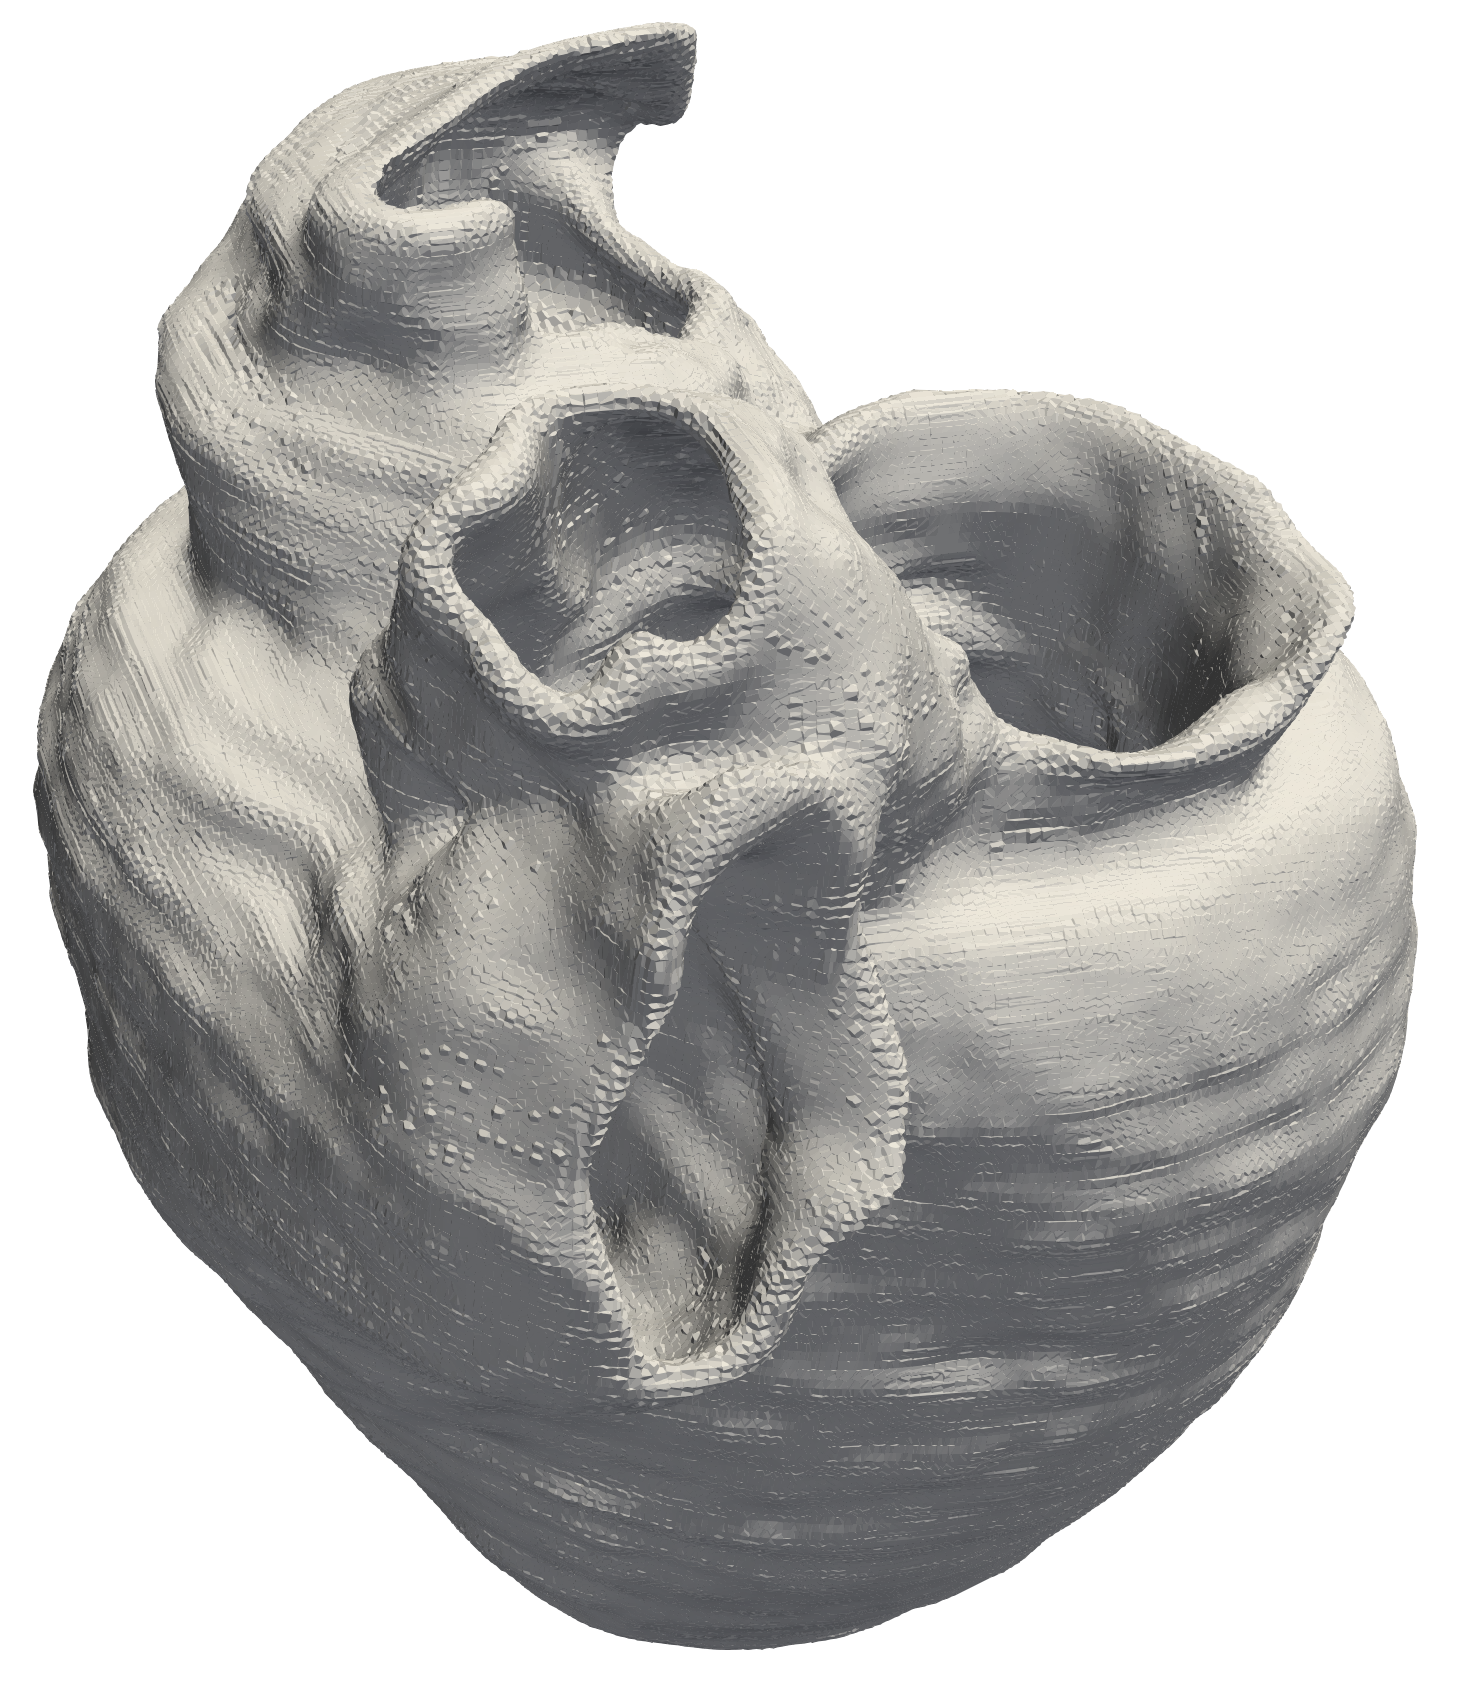
\includegraphics[scale=0.1]{media/2-shabaka/4-clean/1-init.png}
\label{fig:cross2-1}}		
\subfigure[]{%
		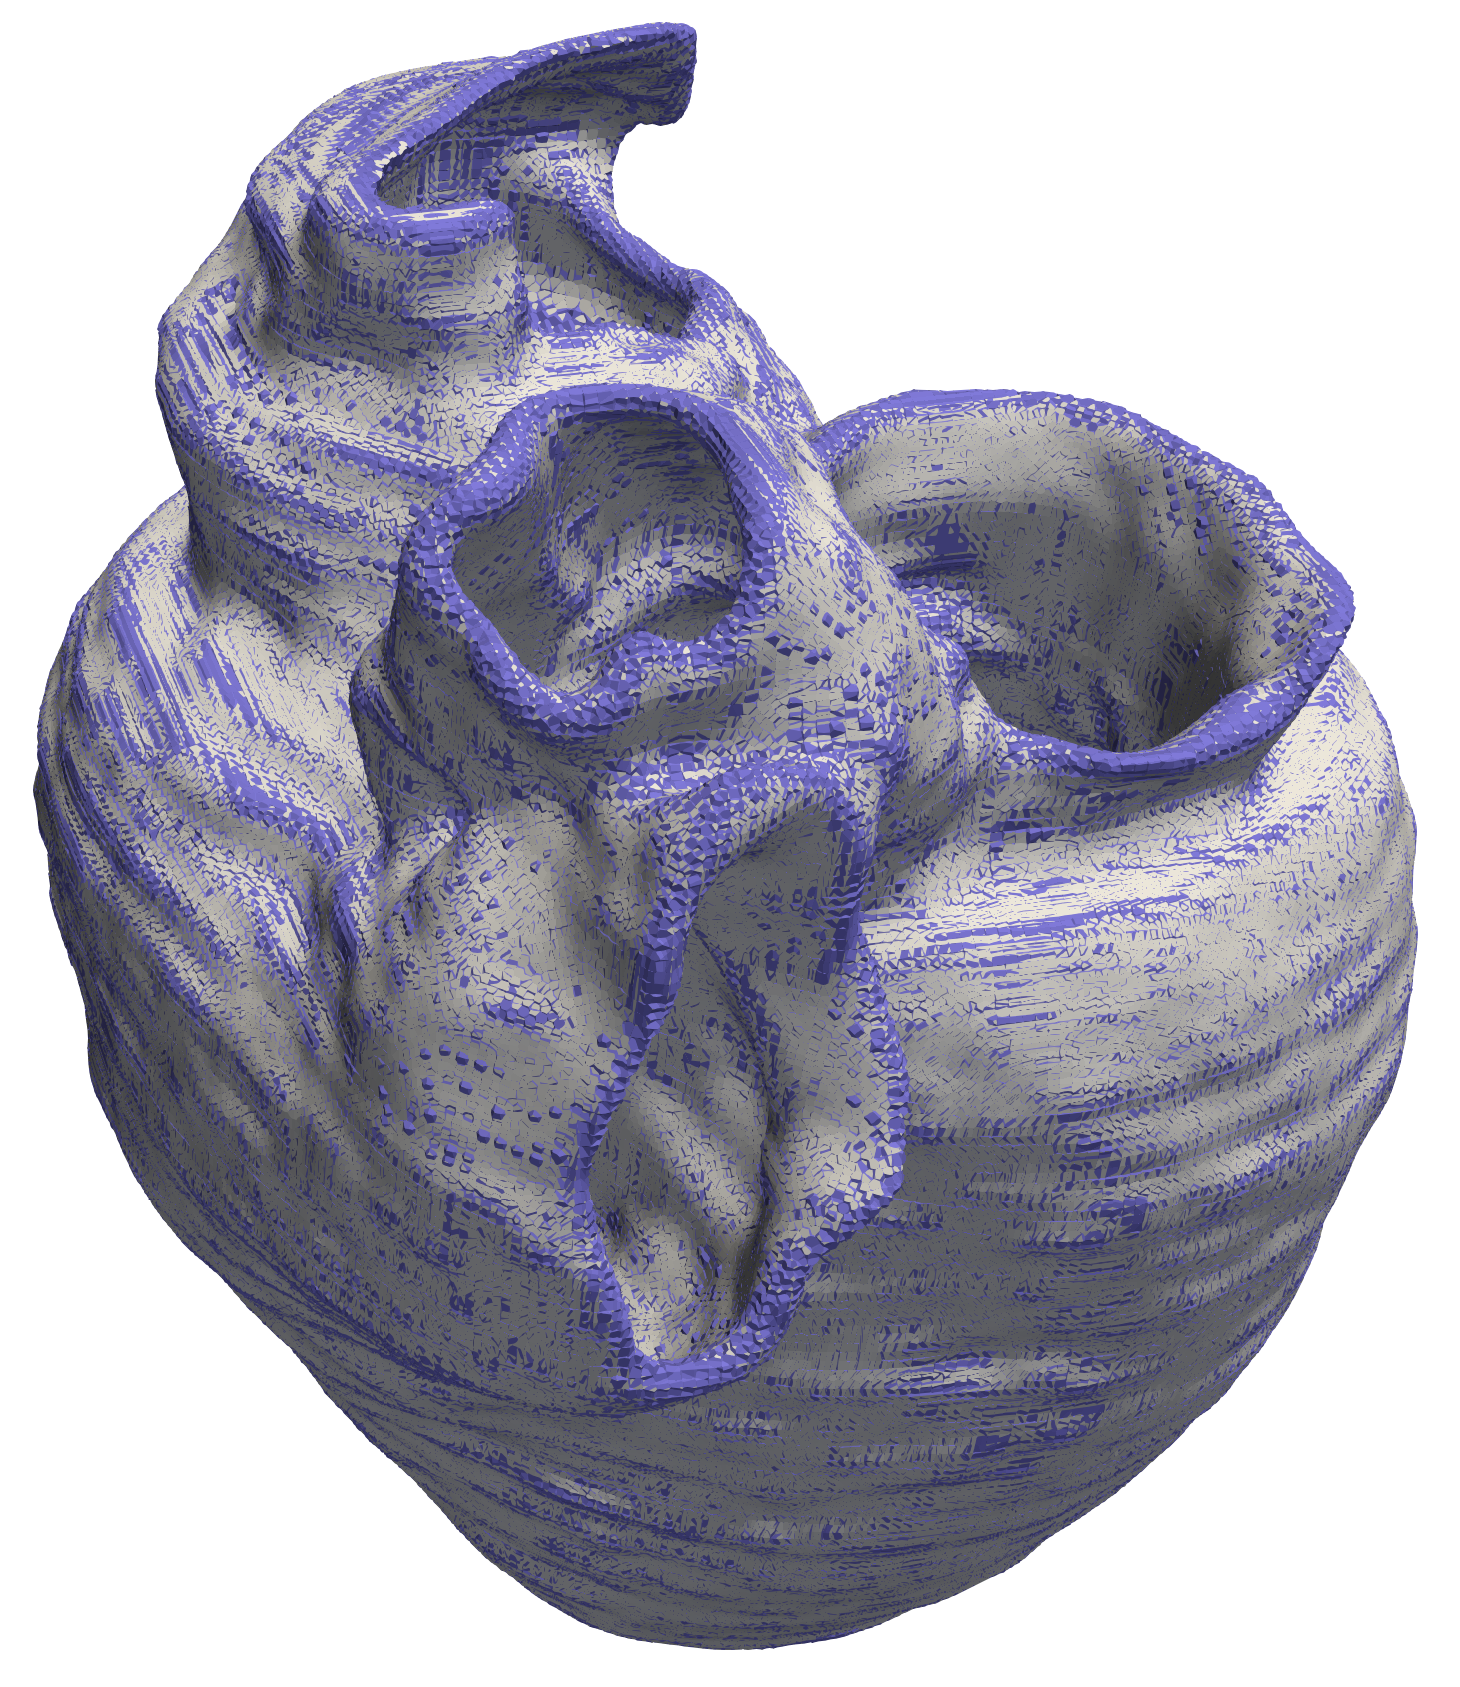
\includegraphics[scale=0.1]{media/2-shabaka/4-clean/2-badfacets.png}
\label{fig:cross2-2}}		
\subfigure[]{%
		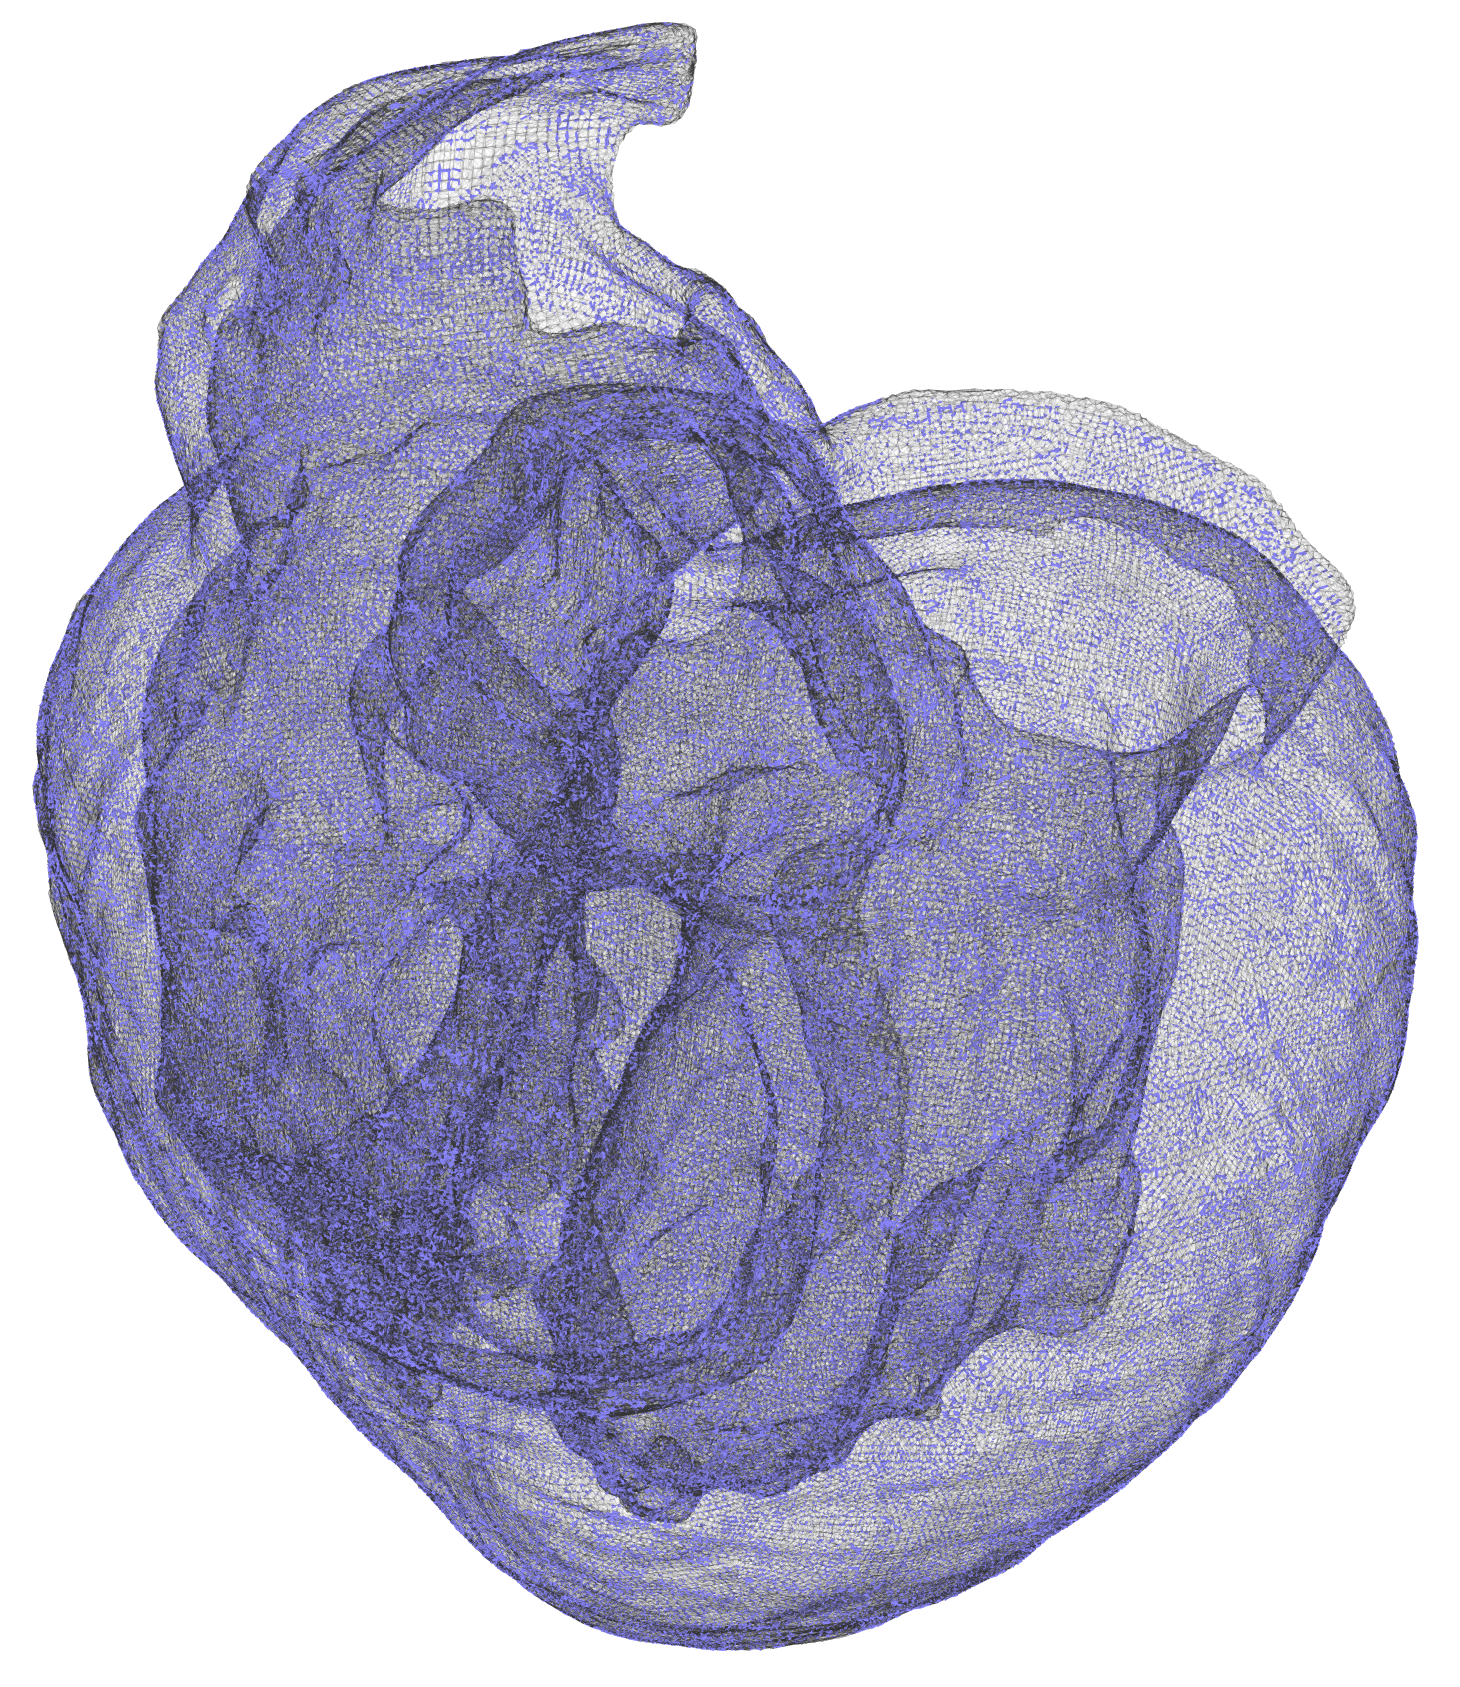
\includegraphics[scale=0.1]{media/2-shabaka/4-clean/3-badsegs.png}	
\label{fig:cross2-3}}						
\subfigure[]{%
		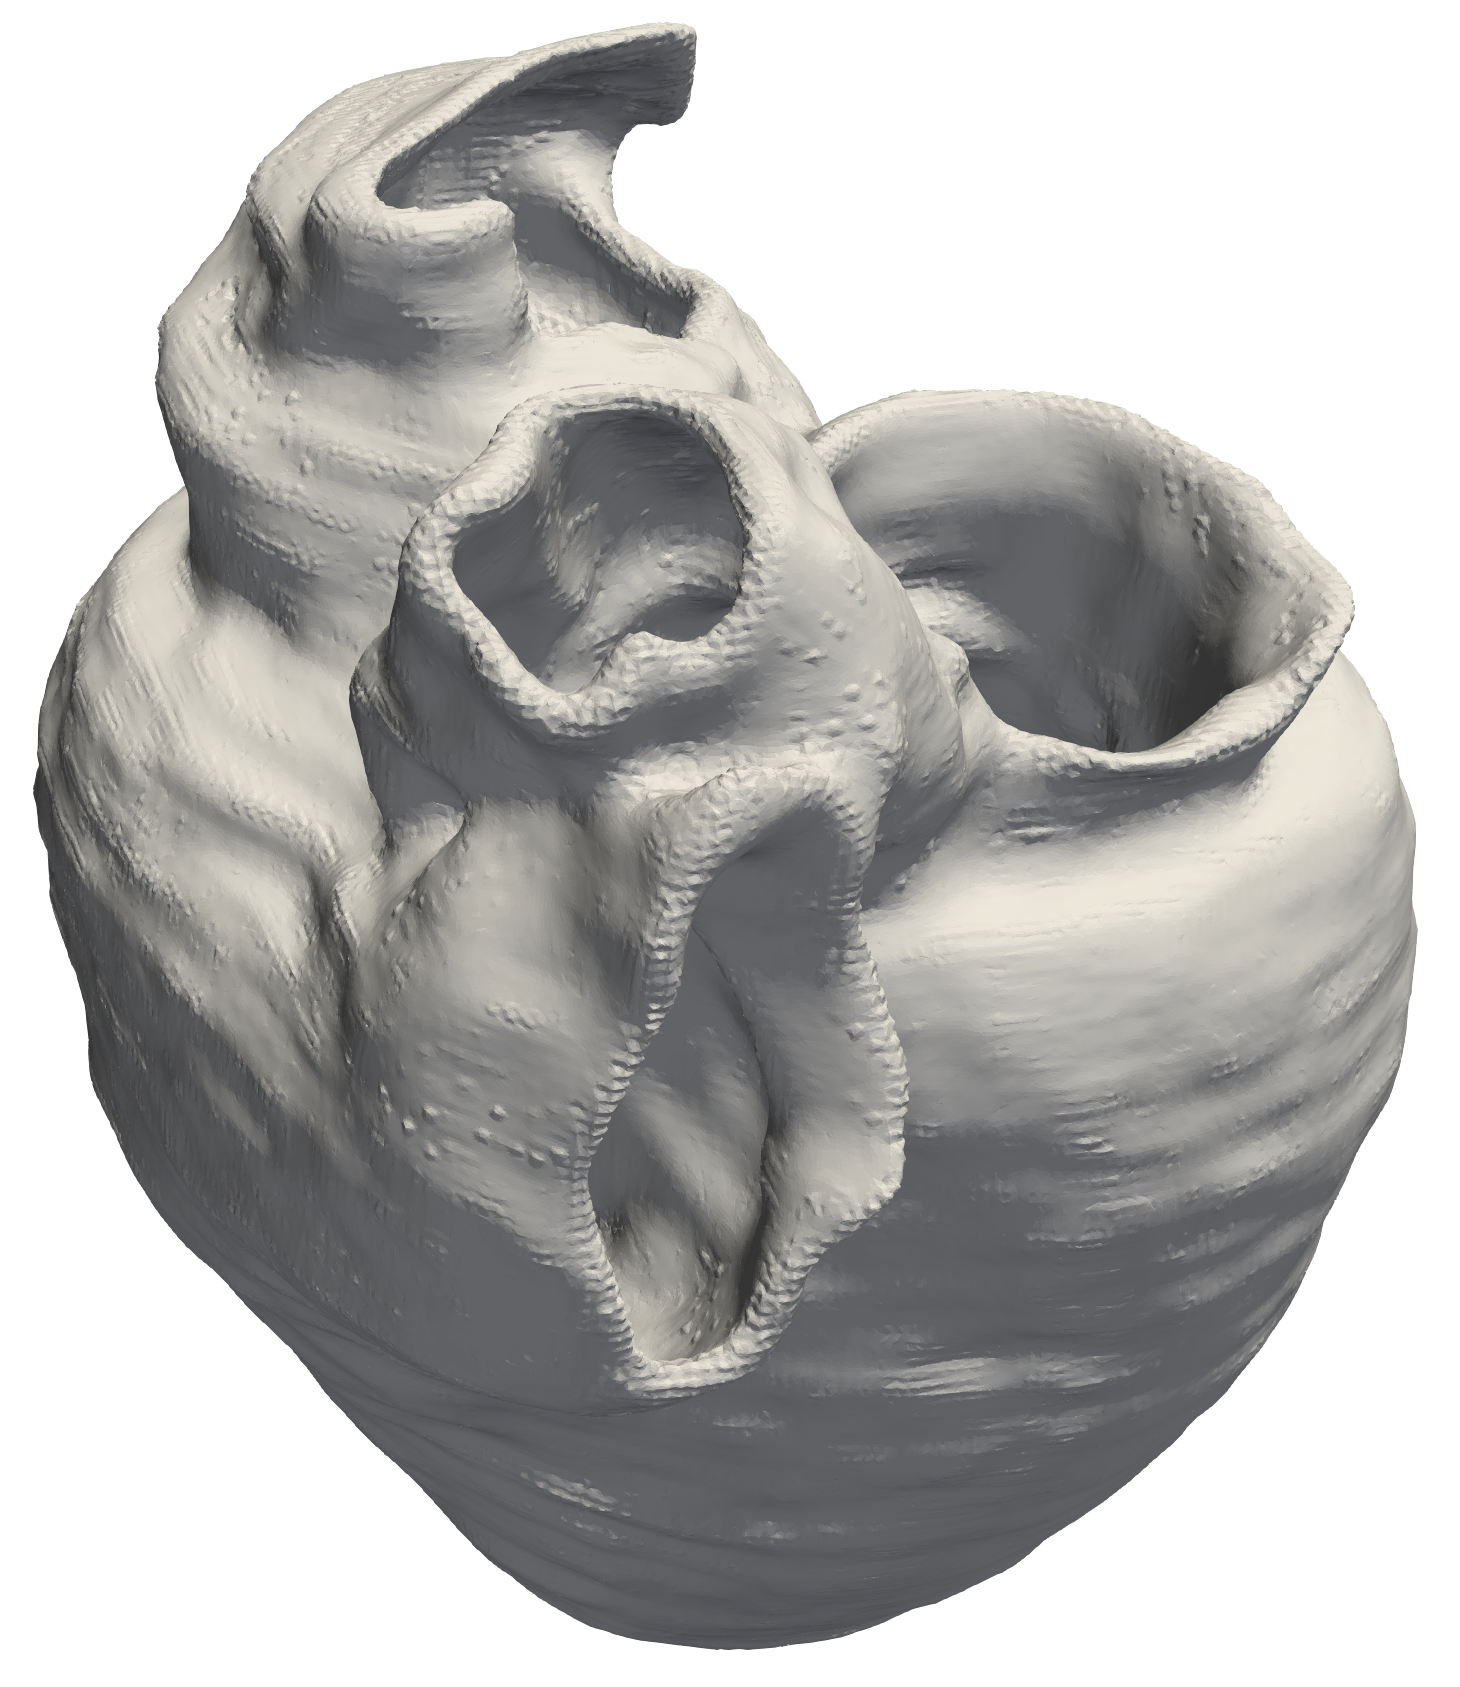
\includegraphics[scale=0.1]{media/2-shabaka/4-clean/4-fine.png}		
\label{fig:cross2-4}}		
%
\caption{Clean-up of undesirable ``cross-talk'' facets for surface of \textit{ex vivo} human heart: (a) initial surface following Voronoi-based surface reconstruction, (b) identification of ``cross-talk'' facets, (c) identification of edges to be collapsed, (d) final cleaned surface}
\label{fig:cross2}
\end{sidewaysfigure}

\subsubsection{Surface Decimation}

Surface \textit{decimation} is performed to reduce the surface mesh to a practical resolution without significantly changing the geometry. The philosophy in image-based meshing, surface extraction, and surface reconstruction is typically to make use of as much information as available to construct a mesh of the highest fidelity possible, and only then to address the practical consideration of mesh resolution for simulation purposes. Indeed, this is what Simpleware's {+FE Free} module does, as described previously. The challenge then becomes decimating in a manner that does not lose more features from the original surface than is desired. For the purposes of this algorithm, decimation is performed using the code \textit{ACVD}~\cite{valette_2004, valette_2008}, which clusters vertices and triangles to generate a coarser surface mesh whose resulting triangles exhibit excellent aspect ratio. The code does not preserve sharp edges or corners, however. This is actually not necessarily an issue for biological structures, as they tend not to have singularities, but would be a problem if the proposed image-based meshing paradigm were extended to meshing mechanical parts from micro-CT scans, for example.

\subsubsection{Results}

Results of the entire surface generation procedure described in this chapter are shown in~\figref{shabakaseq} for the \textit{ex vivo} human heart example. The optimal parameters identified for robust surface generation are shown in~\tabref{Mod5}. The algorithm was rigorously tested with these parameters to produce closed, manifold surfaces for a wide variety of examples. For the \textit{ex vivo} heart, the corresponding point cloud consisted of 236k points, the Voronoi site set comprised of 472k sites, and. the surface mesh prior to decimation yielded 1.00m points and 2.01m triangles. Following decimation the final surface mesh consisted of 50k points and 100k triangles.

\begin{table}[ht!]
 \centering
   \begin{tabular}{|c||c|c|}
   \hline 
   \textbf{Variable} & \textbf{Description} & \textbf{Value} \\ \hline \hline
   $R_{\mathcal{W}}$ & window radius (in voxels) & 5 \\ \hline
   $d_{\mathcal{W}}$ & sampling distance between adjacent windows (in voxels) & 2 \\ \hline
   \multirow{2}{*}{$\overline{k}_{\mathcal{M}}$ \rule{0mm}{4mm}} & threshold for acceptable ratio of voxels in & \multirow{2}{*}{0.925} \\
   {} & window $\mathcal{W}$ belonging to material $m$ & {} \\ \hline
   $\beta_0$ & functional weighting coefficient for zeroth moment of volume & 0.5 \\ \hline
   $\beta_1$ & functional weighting coefficient for first moment of volume & 0.3 \\ \hline   
   $\varepsilon$ & tolerance for minimization of functional $\mathcal{F}$ & $10^{-14}$ \rule{0mm}{4mm} \\ \hline
   $\overline{\mathcal{F}}$ \rule{0mm}{4mm} & largest acceptable value of functional $\mathcal{F}$ & $0.15$ \\ \hline
   \multirow{2}{*}{$b$} & distance between interface normal and & \multirow{2}{*}{$1.1$} \\
   {} & corresponding Voronoi site pair (in voxels) & {} \\ \hline
\end{tabular}
\caption{Optimal parameter values for b-rep generation}
\label{tab:Mod5}
\end{table}

\begin{sidewaysfigure}[htbp!]
\centering
\subfigure[]{%
		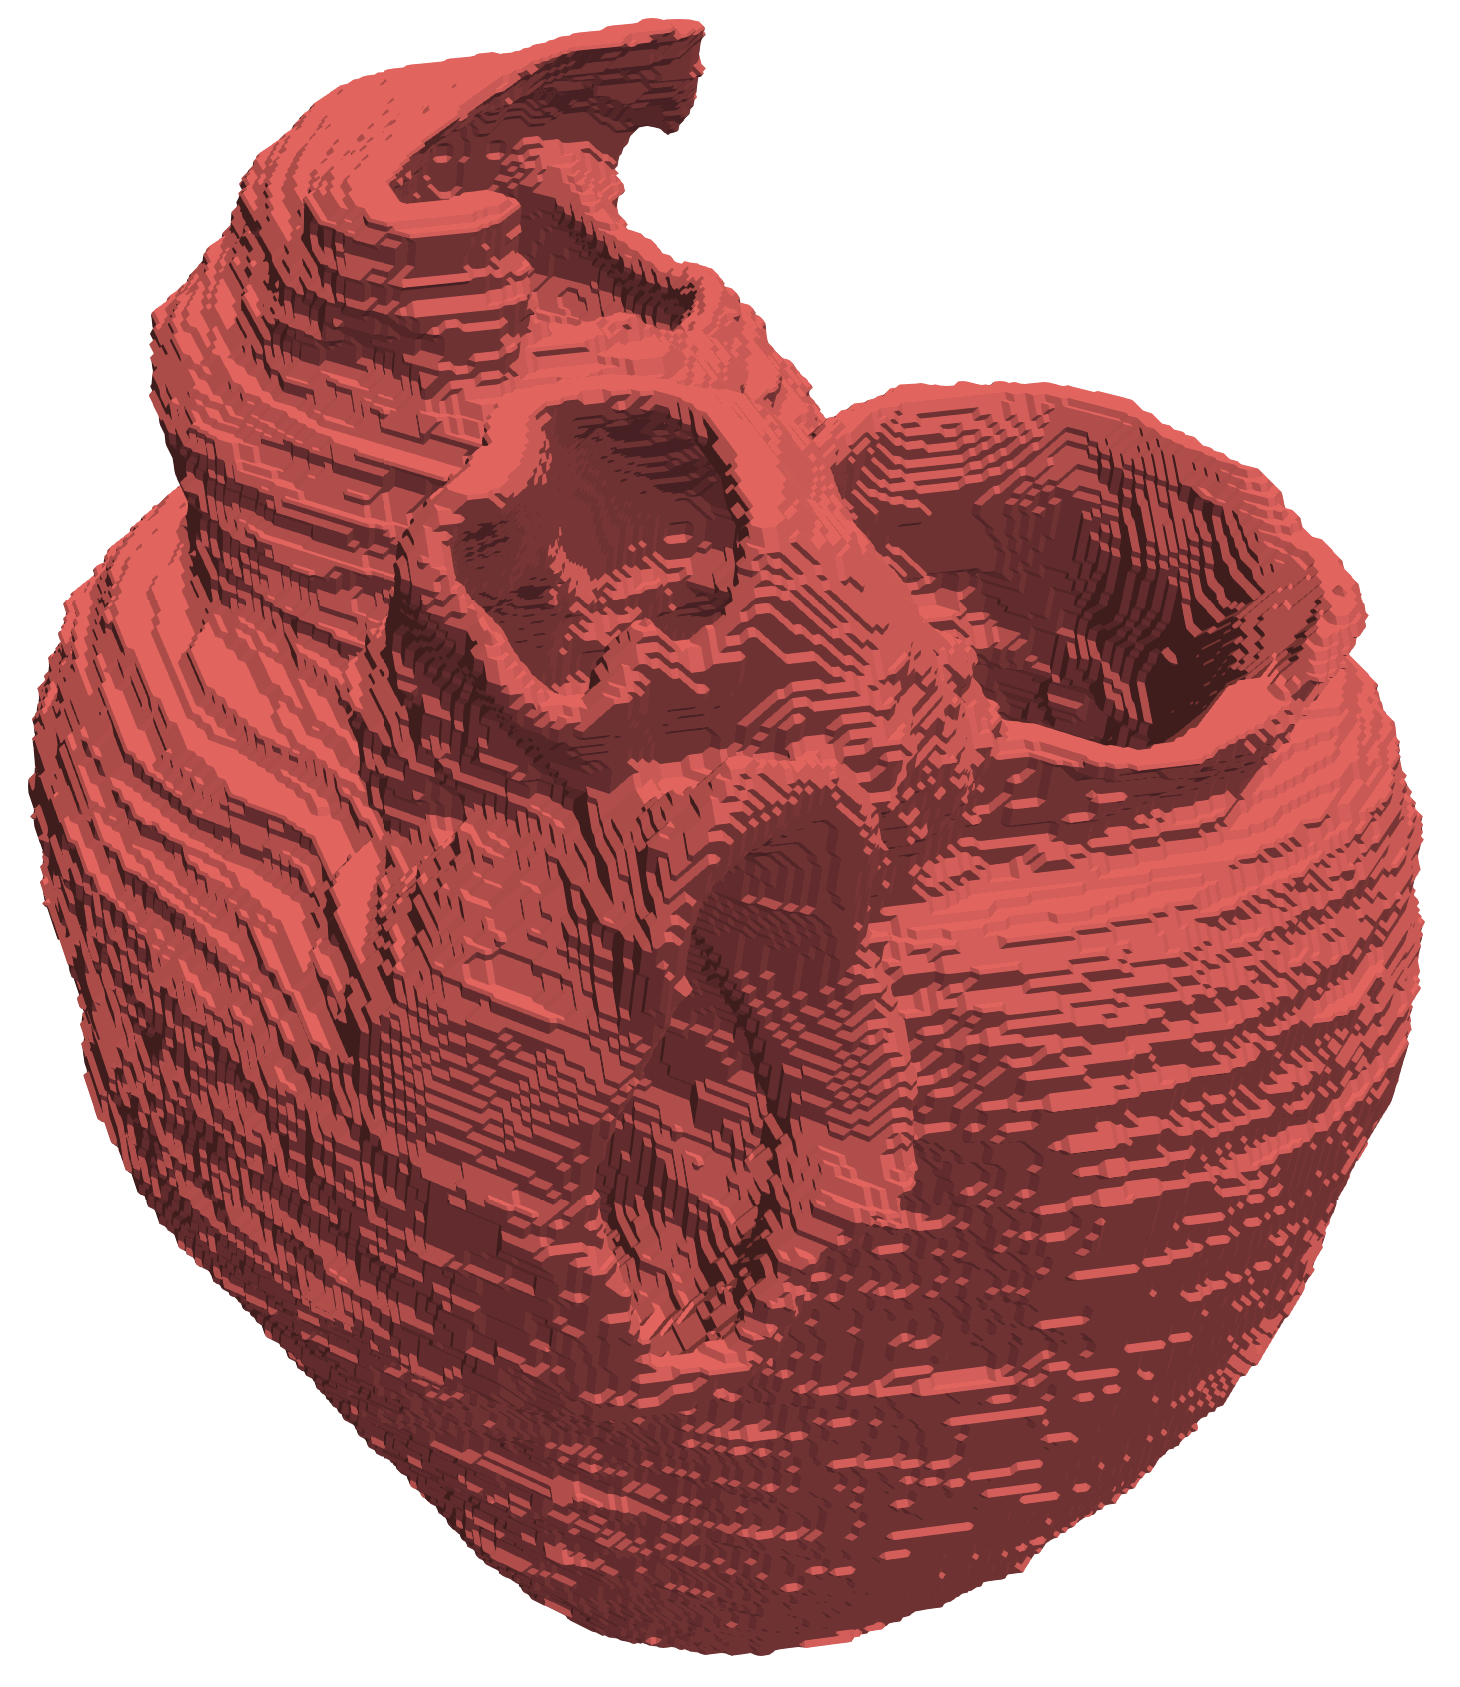
\includegraphics[scale=0.1]{media/2-shabaka/2-surf/1-seg.png}
\label{fig:shabakaseq1}}
\subfigure[]{%
		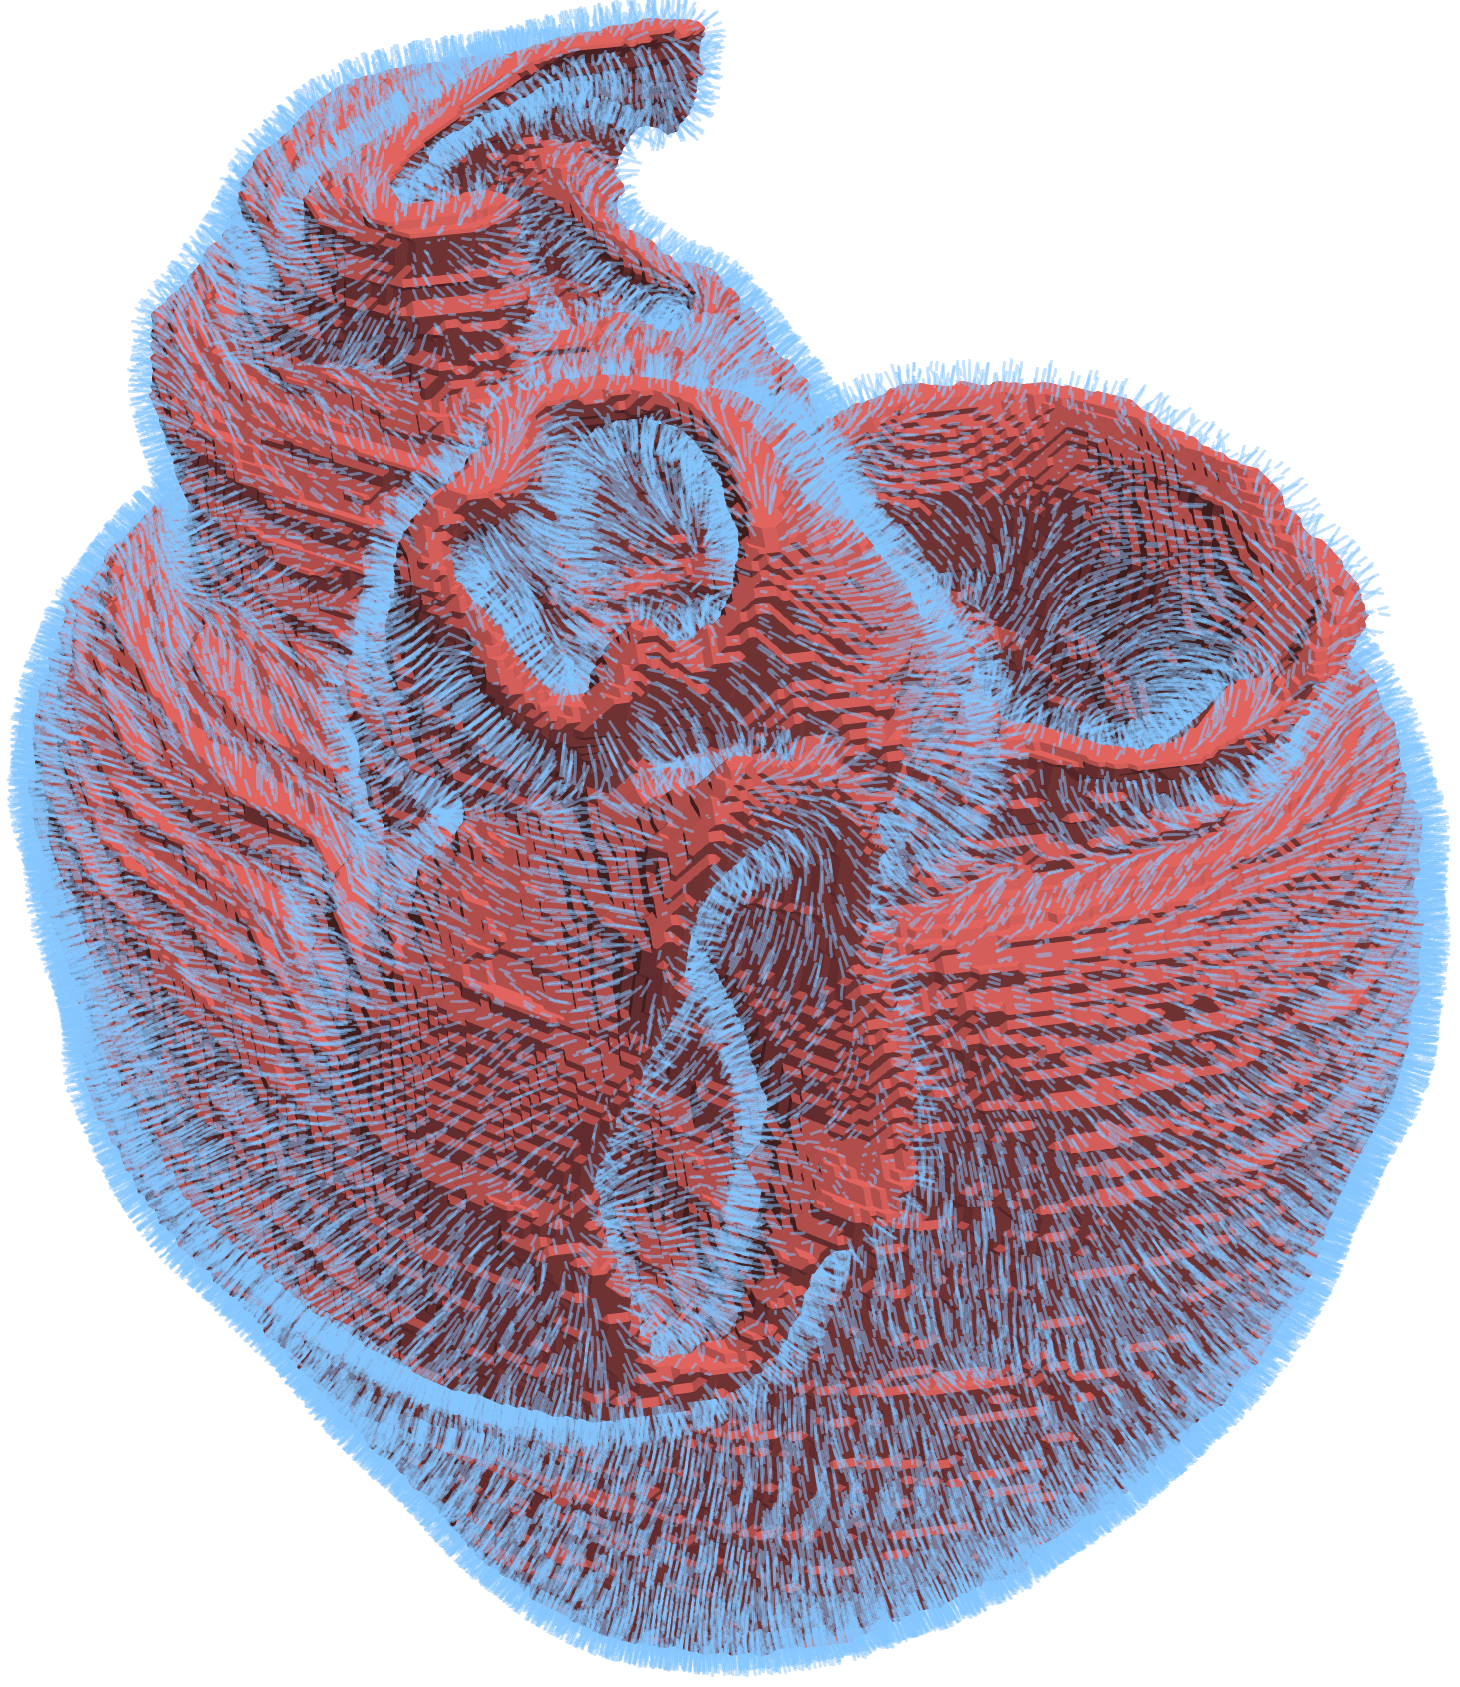
\includegraphics[scale=0.1]{media/2-shabaka/2-surf/2-normals.png}
\label{fig:shabakaseq2}}
\subfigure[]{%
		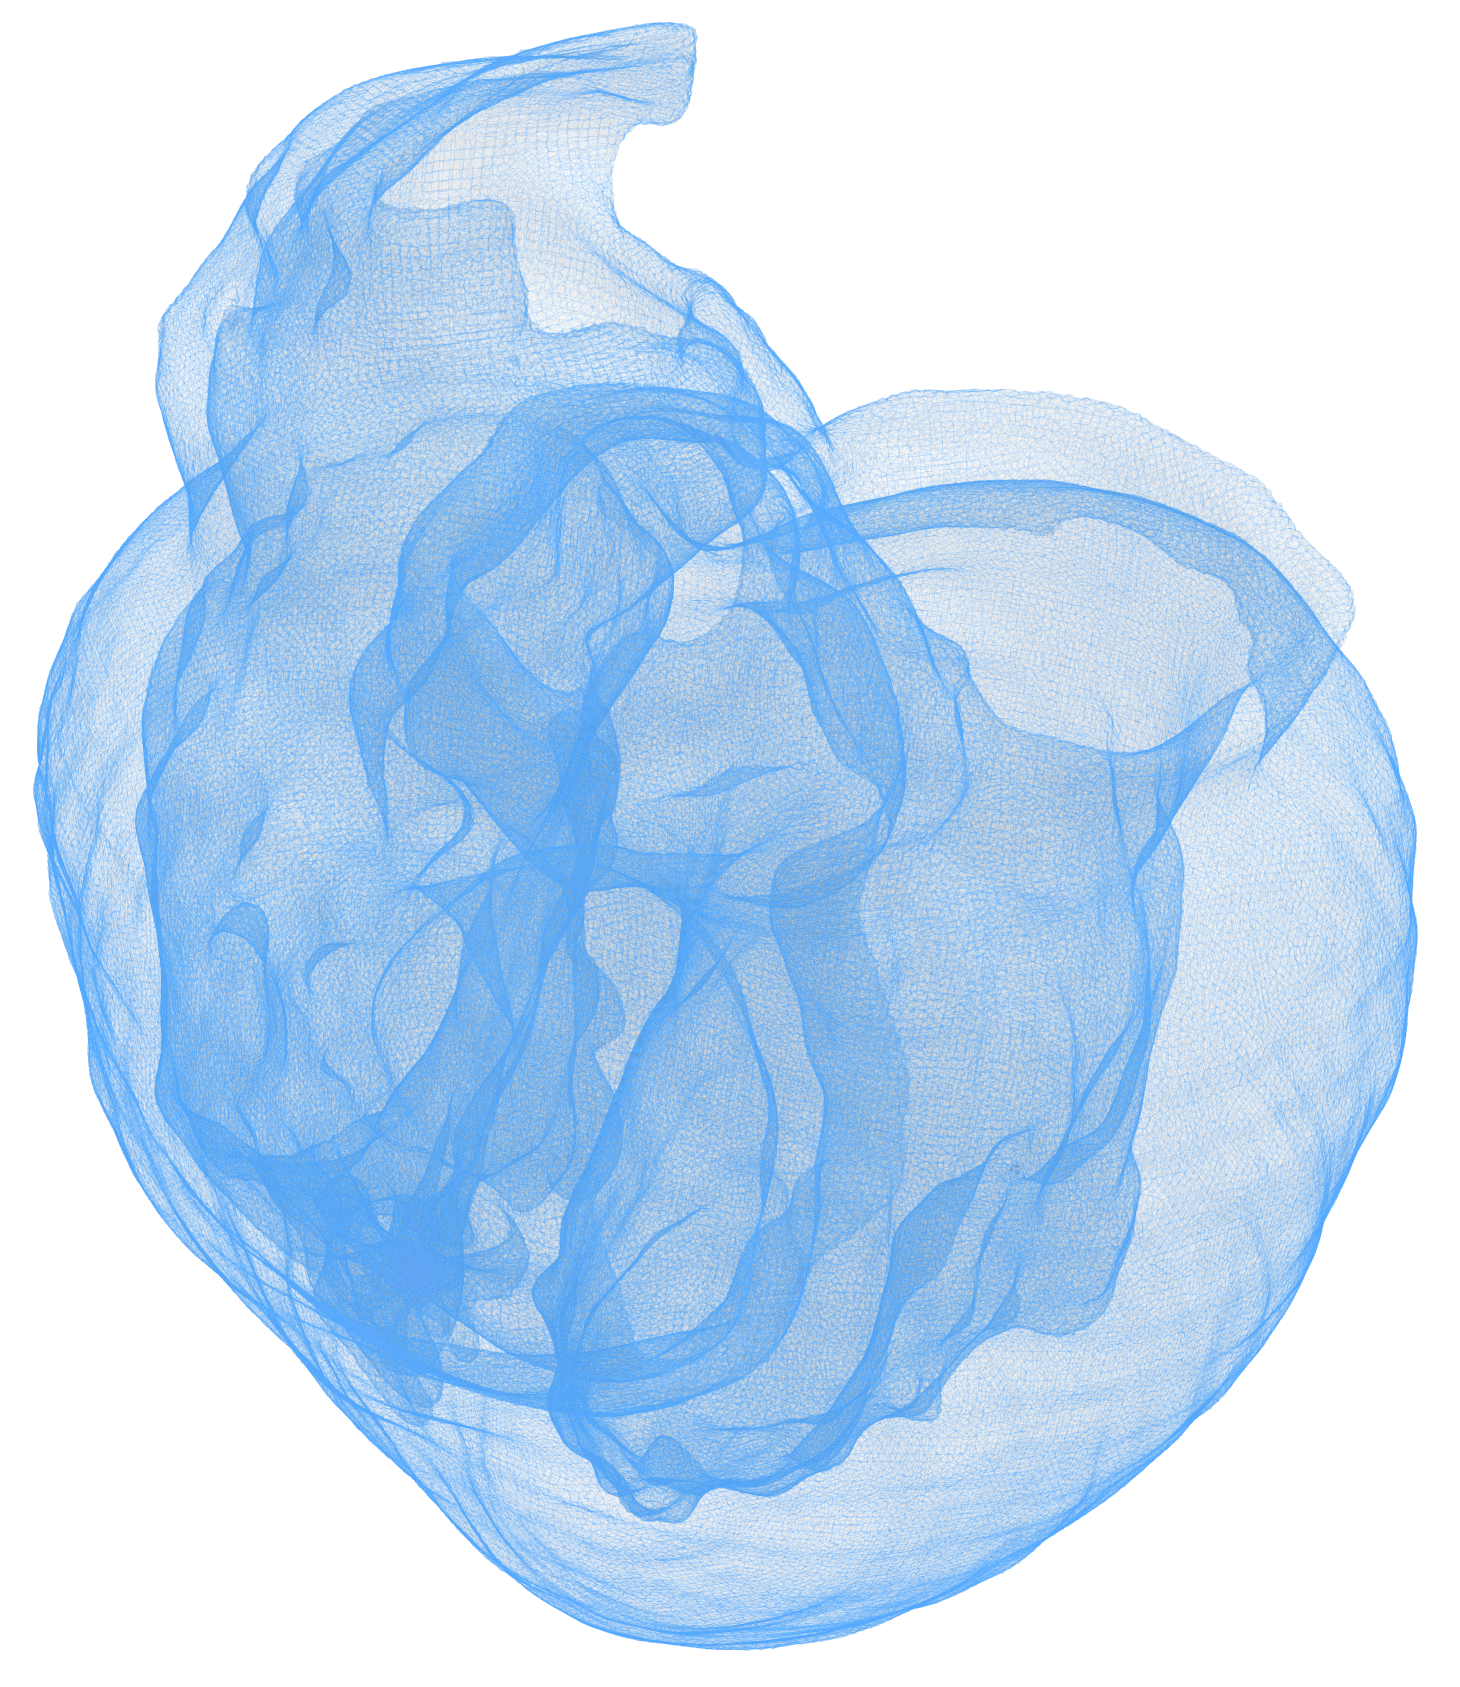
\includegraphics[scale=0.1]{media/2-shabaka/2-surf/3-ptcloud.png}
\label{fig:shabakaseq3}}
\\
\subfigure[]{%
		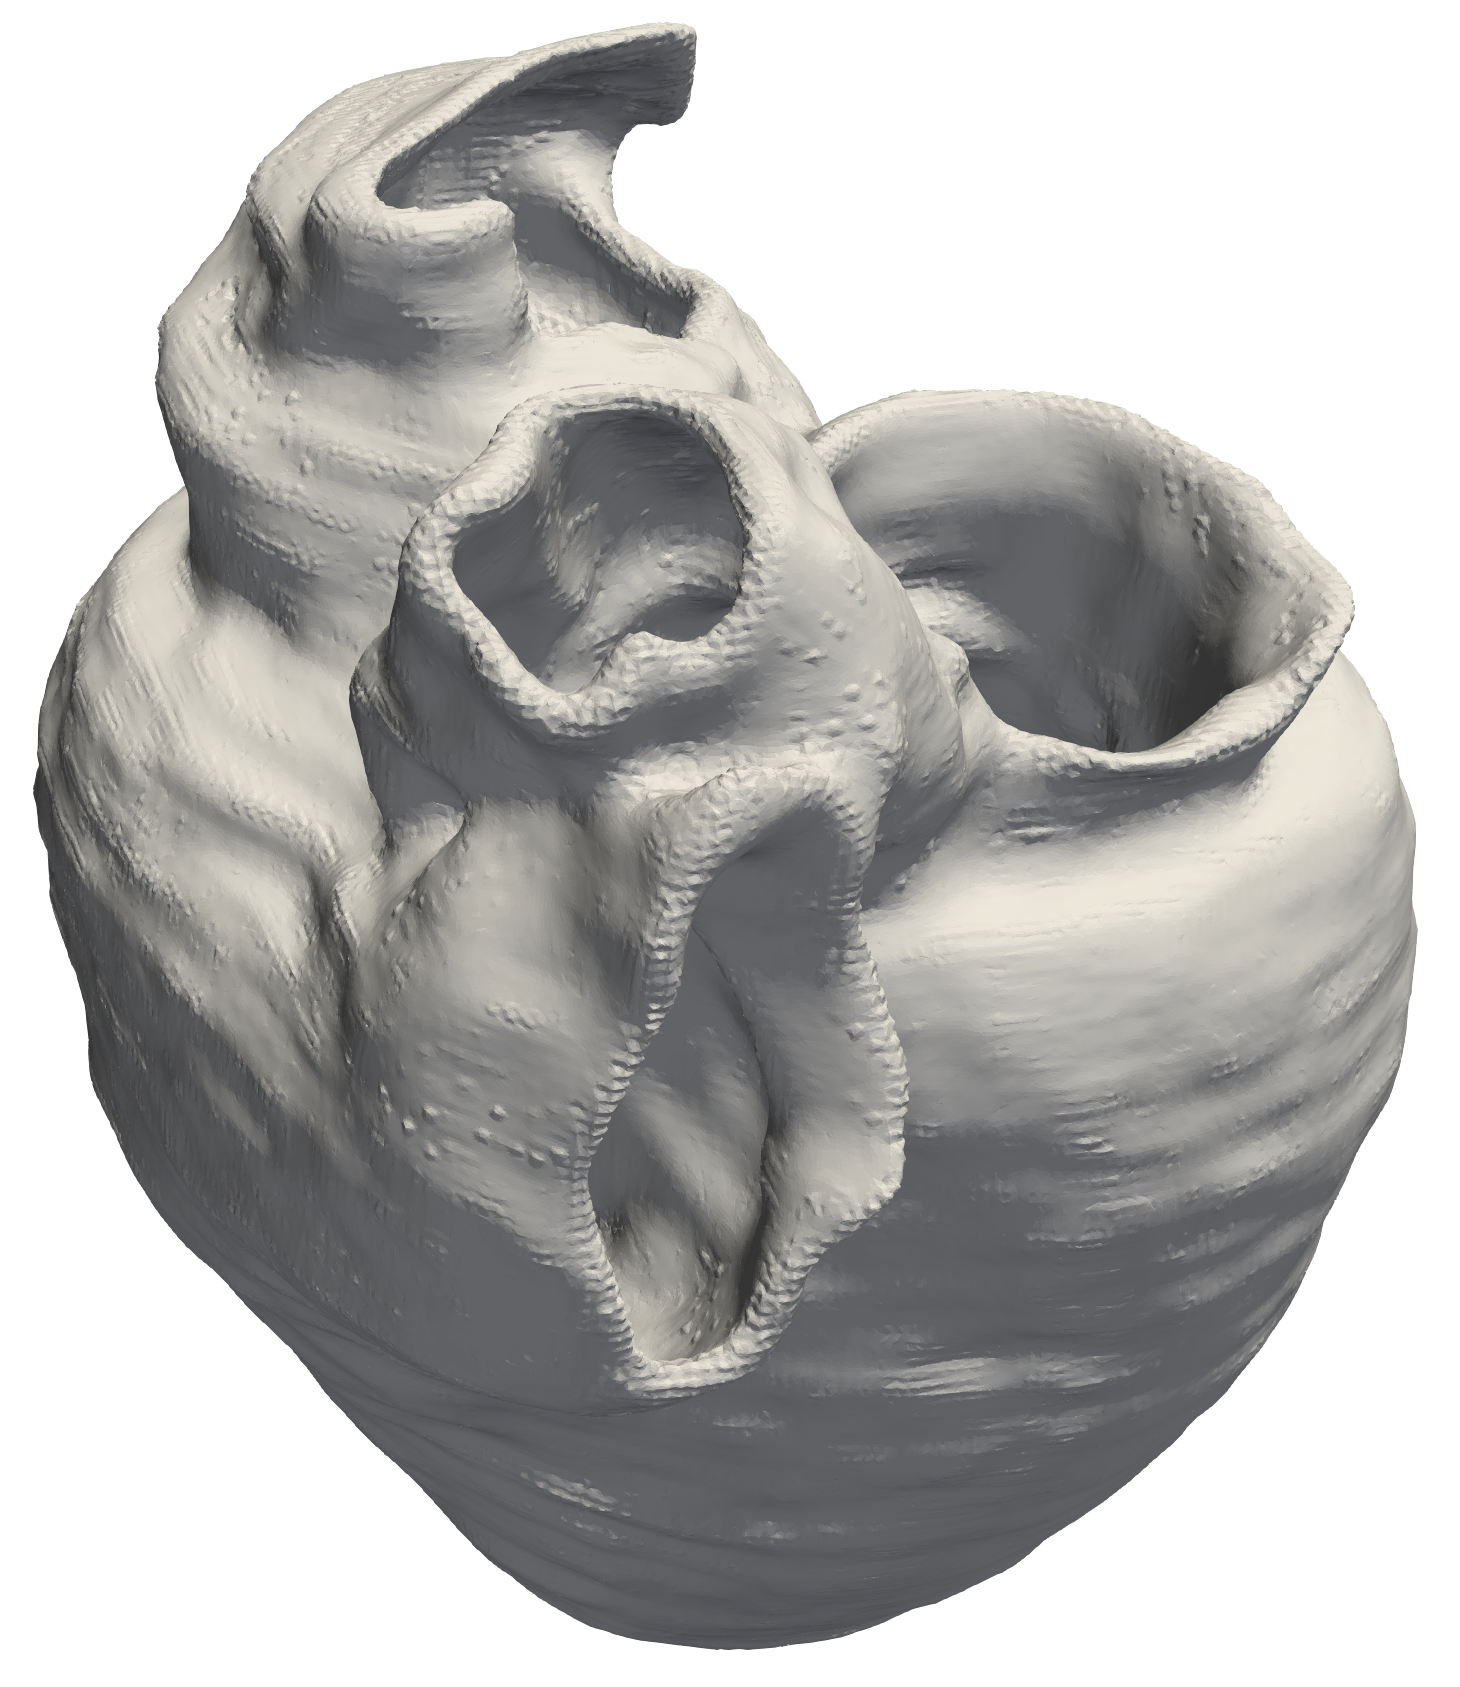
\includegraphics[scale=0.1]{media/2-shabaka/2-surf/4-finesurf.png}
\label{fig:shabakaseq4}}
\subfigure[]{%
		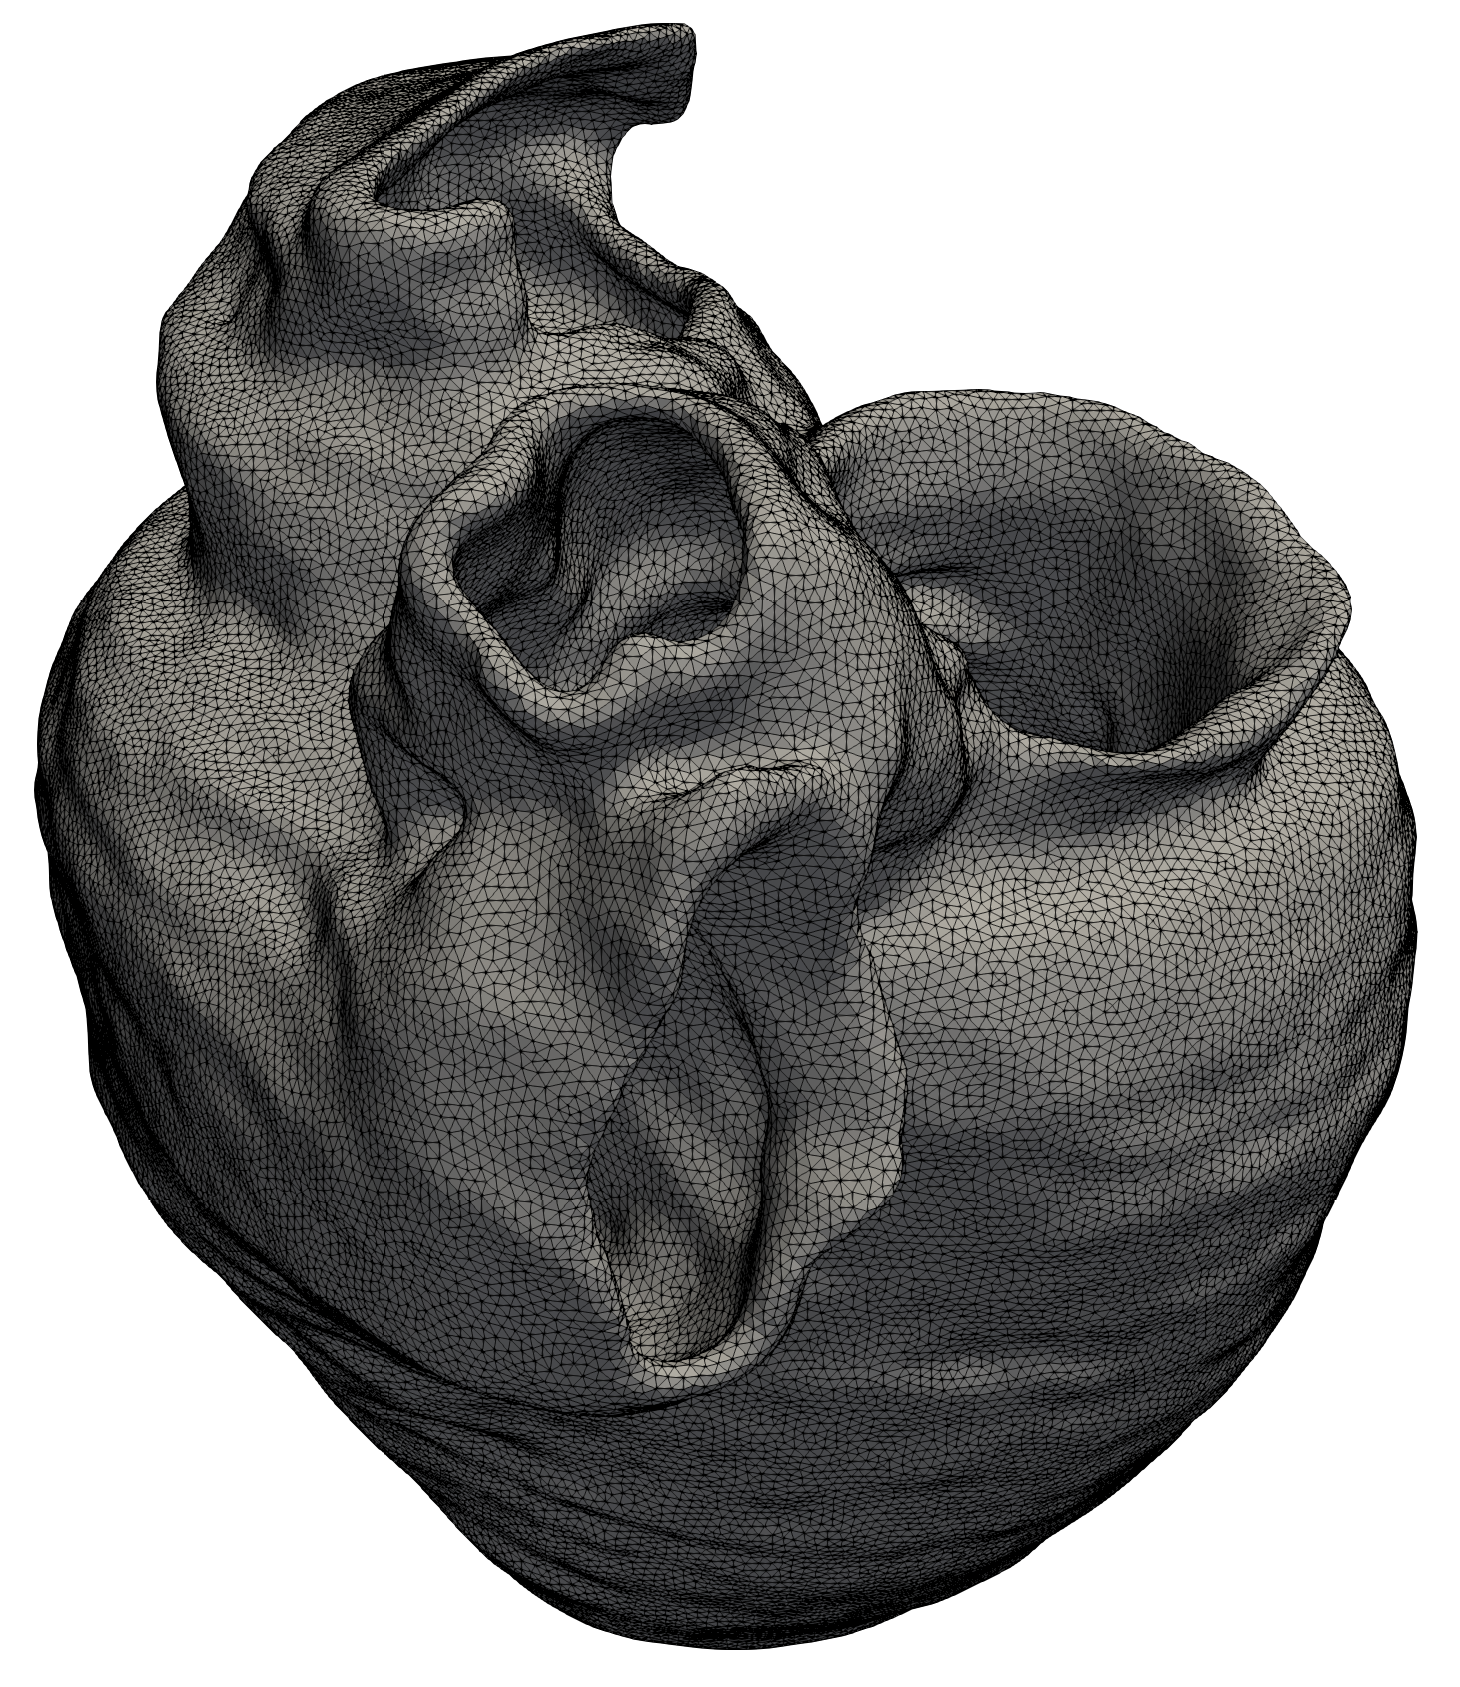
\includegraphics[scale=0.1]{media/2-shabaka/2-surf/5-surf.png}
\label{fig:shabakaseq5}}
%
\caption{(a) Segmented image, (b) point/normal placement, (c) oriented point cloud (normals not shown), c) cleaned surface mesh generated from Voronoi partition (edges not shown), and d) final decimated surface}
\label{fig:shabakaseq}
\end{sidewaysfigure}

%%%%%%%%%%%%%%%%%%%%%%%%%%%%%%%%%%%%%%%%%%%%%%%
%%%%%%%%%%%%%%%%%%%%%%%%%%%%%%%%%%%%%%%%%%%%%%%
\subsection{File Formats}
\label{File Formats-SURF}

Among free software, the simplest and most prevalent file formats for storing point clouds and surface meshes are the Stanford Polygon Format (PLY)~\cite{ply} and the Visualization Toolkit Format (VTK)~\cite{vtk}. Similar to the file format of images and image masks, these formats include a header that describes the data that it precedes. The number of vertices is included in the header, as well as a list of expected point data in the file (e.g., spatial coordinates, normal components). Both file formats handle many different data types (again, \texttt{unsigned char}, \texttt{int}, etc.), so the data type of each piece of data must be prescribed as well. The data itself simply includes vertex coordinates, additional vertex property data if available, and in the case of meshes, the vertex connectivity of facets.

Once again, the raw data may be stored in ASCII or binary format. ASCII format for these point clouds and surface meshes holds significantly more value for these data types than for images or image masks, as specific vertex coordinates and/or connectivities can be queried or even modified. However, for dense point clouds or fine meshes, file sizes can become intractable, and thus binary storage is still the preferred route. Newer editions of the VTK format store data in XML format, but were not explored for the purposes of this work.

The Stereolithography (STL) file format is, unfortunately, still the most popular manner in which surface meshes are stored. STL files store a list of independently defined triangles based on vertex coordinates. Thus, for a closed surface the amount of unnecessarily repeated vertex coordinate data can balloon. The tolerances for which the STL file is generated and subsequently read can cause much more serious problems though. For example, if the tolerance for which the STL is generated is less than that for which it is read (potentially in a different piece of software), the file may be incorrectly deemed non-manifold, and require processing to address the problem. This of course is a non-issue for file formats like PLY and VTK, in which vertices are explicitly defined and numbered in the file, rather than requiring the software reading the file to determine that information.

\section{Mesh Generation}
%
Provided an appropriate surface mesh, CAD-based meshing techniques seek to automatically generate an unstructured discretization of the enclosed volume. Under rare circumstances, the topology of the object of interest may allow for a \textit{structured} mesh, in which there is a predictable repeated connectivity among neighboring elements. To accommodate a surface of arbitrary form, though, an \textit{unstructured} mesh is necessary. The challenge in automated meshing is to maximize the element shape quality while minimizing computational cost or human intervention~\cite{blacker_2001}. The discussion will focus on generating meshes for simulations using finite element methods and its variants. For conventional finite element approaches, topological restrictions on the mesh elements make tetrahedral and hexahedral shapes the most popular choices. Hex and tet meshing approaches have had some success, but not without serious drawbacks. Polyhedral meshing is considered as an alternative, to be used in conjunction with polyhedral finite element methods. Established meshing techniques are summarized, together with a demonstration of the advantages of the polyhedral approach.

%%%%%%%%%%%%%%%%%%%%%%%%%%%%%%%%%%%%%%%%%%%%%%%
%%%%%%%%%%%%%%%%%%%%%%%%%%%%%%%%%%%%%%%%%%%%%%%
\subsection{Hexahedral Meshing}
\label{Hexahedral Meshing}

In general, hexahedral meshes produce the most accurate solutions in finite element simulations, and are more computationally efficient than its alternatives~\cite{tautges_2001}. Additionally, for problems involving near-incompressibiliy, mitigation strategies for volumetric locking like \textit{F-bar projection} are more developed and tested for linear 8-node hexes compared to, say, higher order tetrahedra. To date, though, no algorithm exists that can perform automatic hexahedral meshing of surfaces with arbitrary geometry and topology. The difficulty lies in the strict nodal connectivity constraints that require the hexahedral discretization to consist of either stacks of elements or closed loops~\cite{young_2008}. 

Among the most popular classes of hexahedral meshing techniques are: \textit{primitives}, \textit{overlay grid}, and \textit{automated decomposition}~\cite{blacker_2001}. \textit{Primitives} typically involve producing a 2D unstructured quad mesh of a cross section, followed by \textit{sweeping} the constant topology cross section. This approach is limited to topologies involving a swept cross-section. \textit{Overlay grids} produce a structured background grid, and cut elements and/or modify vertices so that the hex elements near the surface conform to the original surface. However, this approach can lead to elements with potentially very poor quality. \textit{Automated decomposition} techniques attempt to decompose the volume into separate parts that are subsequently meshed based on swept volumes or other primitive shapes. Decomposing the surface typically requires some degree of manual guidance, though. These approaches suffer from difficulty in matching meshes at part interfaces, and require potentially significant user-driven de-featuring of the surface.

Hexahedral meshing algorithms typically only apply to a limited set of geometries. In practice, human intervention is necessary to decompose the geometry according to the algorithms available, adjust the geometry as needed to accommodate those algorithms, and - much like image segmentation - potentially select between a suite of tools to be employed as needed~\cite{blacker_2001}. These manual efforts can become impracticably time consuming or even impossible for surfaces of biological tissues, and thus fully hex meshes are not typically used in biomechanics applications.

Mixed element approaches attempt to alleviate the difficulty of producing fully hexahedral meshes by only requiring the mesh to be \textit{hex dominant}. In hex dominant meshes, tetrahedra exist where a hexahedral mesh is intractable, and pyramid elements are required in the transitional layers between hexes and tets. These techniques tend to either: convert an already existing tetrahedral mesh to a hex-dominant mesh by combining tetrahedral elements~\cite{baudouin_2014, gao_2017}; attempt to honor the surface with tetrahedral elements together with an octree hexahedral representation in the interior of the volume~\cite{young_2008, lobos_2015}; or insert tetrahedral elements toward the interior of the volume where frontal approaches of purely hex meshes fail~\cite{blacker_2001}. These approaches have shown promise in meshing arbitrary domains, but little work has been done in evaluating the accuracy and performance in a finite element setting in comparison to fully hex or fully tet meshes~\cite{tautges_2001}.

%%%%%%%%%%%%%%%%%%%%%%%%%%%%%%%%%%%%%%%%%%%%%%%
%%%%%%%%%%%%%%%%%%%%%%%%%%%%%%%%%%%%%%%%%%%%%%%
\subsection{Tetrahedral Meshing}
\label{Tetrahedral Meshing}

The two most widely adopted approaches for automated unstructured tetrahedral mesh generation are \textit{advancing front} and \textit{Delaunay tetrahedralization}~\cite{lohner_1997}. In advancing front techniques~\cite{jin_1993, lohner_1988}, elements are inserted one at a time, starting from the initial triangular surface mesh and working toward the interior of the enclosed volume. Care must be taken to avoid poor element quality when the front collides from different directions. The success of the approach depends on the initial quality and size of the triangular surface mesh, which can be remedied by surface remeshing/decimation.

Delaunay tetrahedralization is the dual of the previously described \textit{Voronoi diagram}. Namely, the Voronoi sites form the vertices of the Delaunay tetrahedralization, whose edges perpendicularly pass through the coresponding shared Voronoi facets. The set of tetrahedra satisfy the property that no other vertex is contained within the circumsphere formed by the vertices of each tetrahedron. The Delaunay tetrahedralization is typically constructed incrementally. A tetrahedralization is carried out on an initial point distribution. Additional points are introduced and tetrahedra encompassing the new point are removed. The void created by the deletion of these tetrahedra is then remeshed~\cite{young_2008}. The specification of the initial point distribution and subsequent insertion of points dictates the resulting quality of the mesh elements. Constraining the Delaunay tetrahedralization to adhere to the input surface can also severely affect element quality and even produce sliver elements~\cite{lohner_1997}.

A Delaunay meshing implementation from \textit{Tetgen}~\cite{tetgen} is utilized to generate high quality tetrahedral meshes of linear or quadratic order that exactly honor input surface meshes. A tetrahedral mesh of the ventricles of the \textit{ex vivo} heart example is shown in \figref{tetmesh}.

\begin{sidewaysfigure}[htbp!]
\centering
\subfigure[]{%
		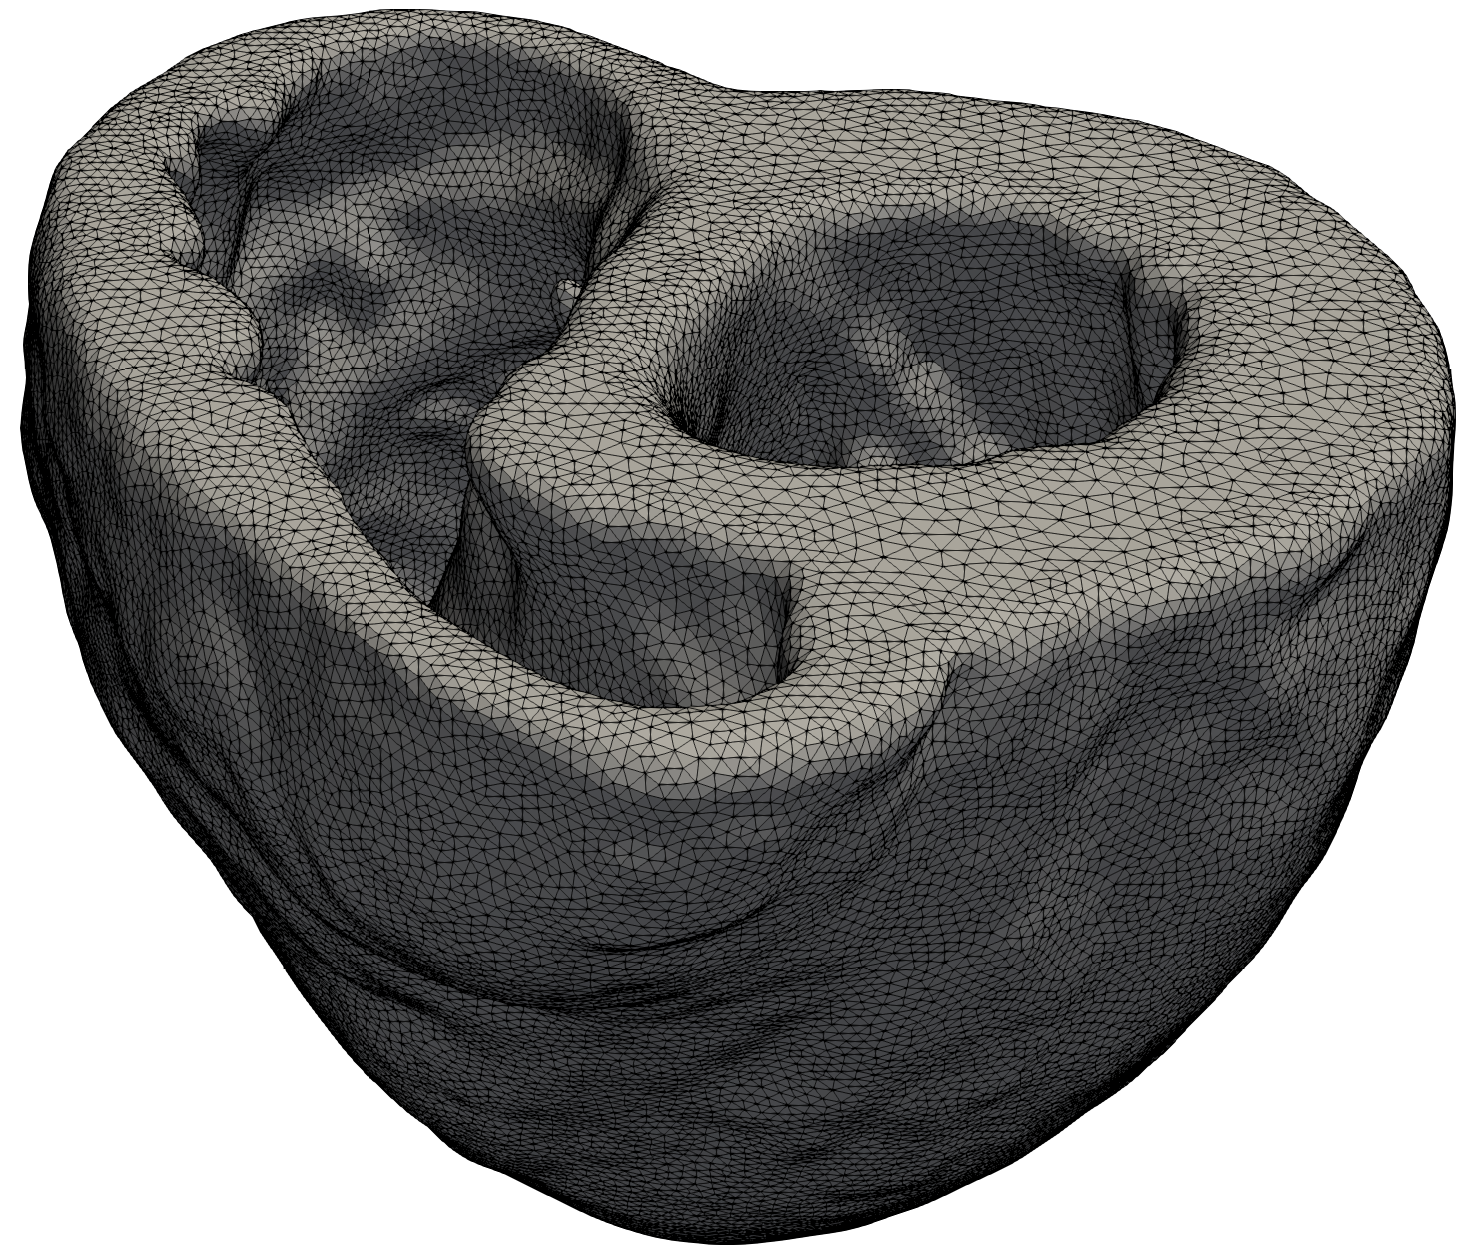
\includegraphics[scale=0.16]{media/4-cardioid/0-ventriclesurf.png}
\label{fig:tet1}}
\subfigure[]{%
		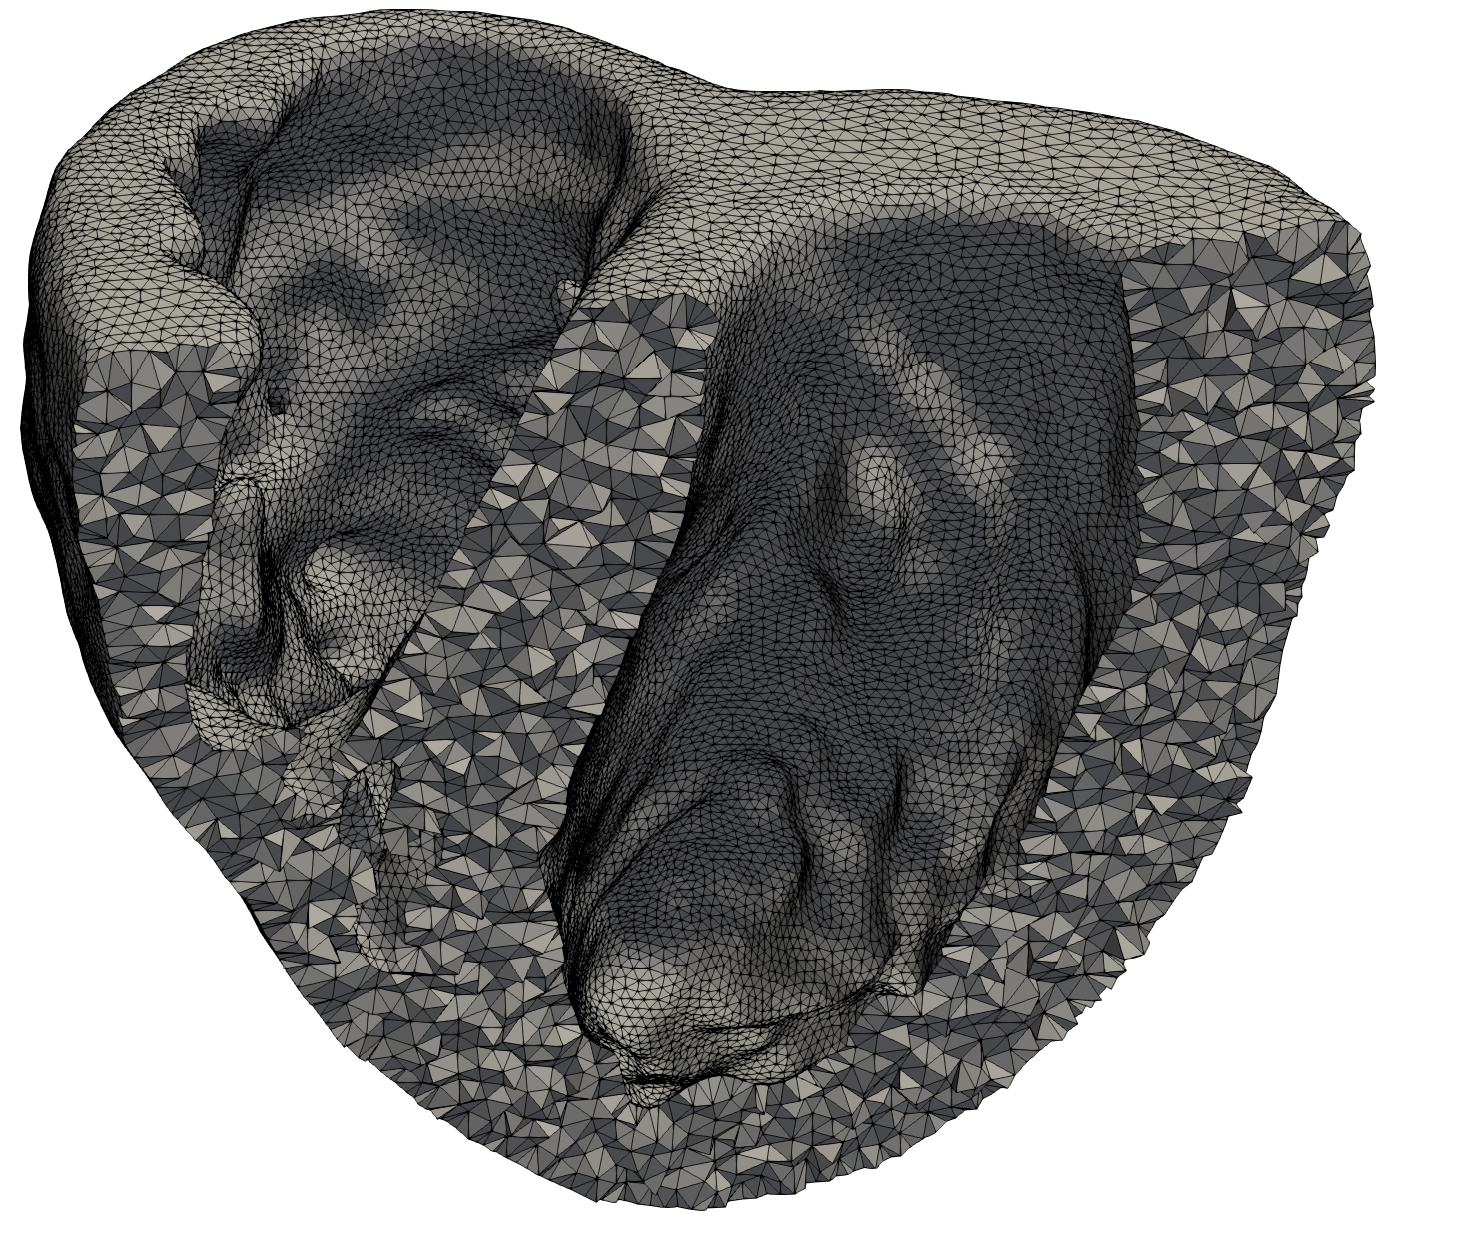
\includegraphics[scale=0.16]{media/4-cardioid/1-tet.png}
\label{fig:tet2}}
%
\caption{Bi-ventricular mesh of \textit{ex vivo} human heart: (a) input surface mesh, and (b) clipped view of quadratic tetrahedral mesh}
\label{fig:tetmesh}
\end{sidewaysfigure}

%%%%%%%%%%%%%%%%%%%%%%%%%%%%%%%%%%%%%%%%%%%%%%%
%%%%%%%%%%%%%%%%%%%%%%%%%%%%%%%%%%%%%%%%%%%%%%%
\subsection{Polyhedral Meshing}
\label{Polyhedral Meshing}

Although hexahedral meshes are generally preferred for conventional finite element approaches, to date there are no techniques available that offer a robust automatic pipeline to generate hex meshes. Thus, tetrahedral mesh generation tools are typically the de facto choice for image-based meshing. Linear tet elements can only represent a constant strain, however, leading to inaccurate solution approximation unless impractically fine meshes are used. Generally speaking, linear tets are not to be used for nonlinear solid mechanics problems involving near-incompressibility~\cite{hughes_2007}, tension, torsion, bending~\cite{wang_2004, benzley_1995}, or contact~\cite{maas_2016}. Quadratic tets, on the other hand, produce much more accurate results and are generally the most popular element choice for biological applications. For problems involving complex geometries and/or requiring high fidelity solutions, though, the resulting problem size for quadratic tet meshes can be problematic. Polyhedral meshes, in conjunction with polyhedral finite element methods, attempt to compete with the robustness of tetrahedral meshes and the accuracy and computational efficiency enjoyed when using hexahedral meshes.

Polyhedral meshing approaches tend to fall under two categories: those that seek to produce a Voronoi partition of the domain, and those that seek a hex-dominant mesh. Meshing techniques that seek to generate Voronoi partitions~\cite{garimella_2014, lee_2015} offer the advantage of exclusively convex elements with desirable aspect ratios. However, this comes at the price of needing to remesh the surface, which re-opens the issue of feature preservation. Indeed, Ebeida \textit{et al.}~\cite{ebeida_2011, mitchell_2015} for example, strategically sampled the input surface mesh before reconstructing it. Special care must be taken to sample regions of high curvature and sharp corners, and these features are not well preserved for some of the examples shown in their work. Additionally, for more general CAD-based meshing applications, it may be desirable to preserve the input surface mesh even if all features are honored exactly, for the purposes of applying boundary conditions or mating adjacent parts later.

Hex-dominant polyhedral meshing ``sculpts'' a background hex mesh with the input b-rep, producing hexahedra on the interior and arbitrary polyhedral shapes near the surface. These arbitrary polyhedra are accommodated by an element formulation that deviates from the conventional FEM approach, to be discussed in~\chapref{4}. This sculpting approach must handle geometric near-degeneracies in a robust way. Indeed, topological correctness is the highest priority if one is to guarantee a simulation-ready mesh for an arbitrary input surface. An implementation of such an approach in the polyhedral FEM software \textit{Celeris} is used to generate polyhedral meshes from input b-reps~\cite{rashid_2013}. To avoid undesirably small elements, the intersection calculation between the input b-rep and its corresponding bounding hex mesh is tolerance-driven. Each polytope of the b-rep and bounding hex mesh is stored via a recursive definition of lower dimensional polytopes, and thus intersections are calculated in stages from lower order polytopes to higher order. In this manner, intersections of dimension greater than zero only require integer logic, and floating point calculations are kept to a minimum~\cite{rashid_2013}. \figref{cel} illustrates the robust polyhedral meshing sequence, and~\figref{zoom} shows some example arbitrary polyhedral elements for which a novel element formulation is required.

\begin{sidewaysfigure}[htbp!]
\centering
\subfigure[]{%
		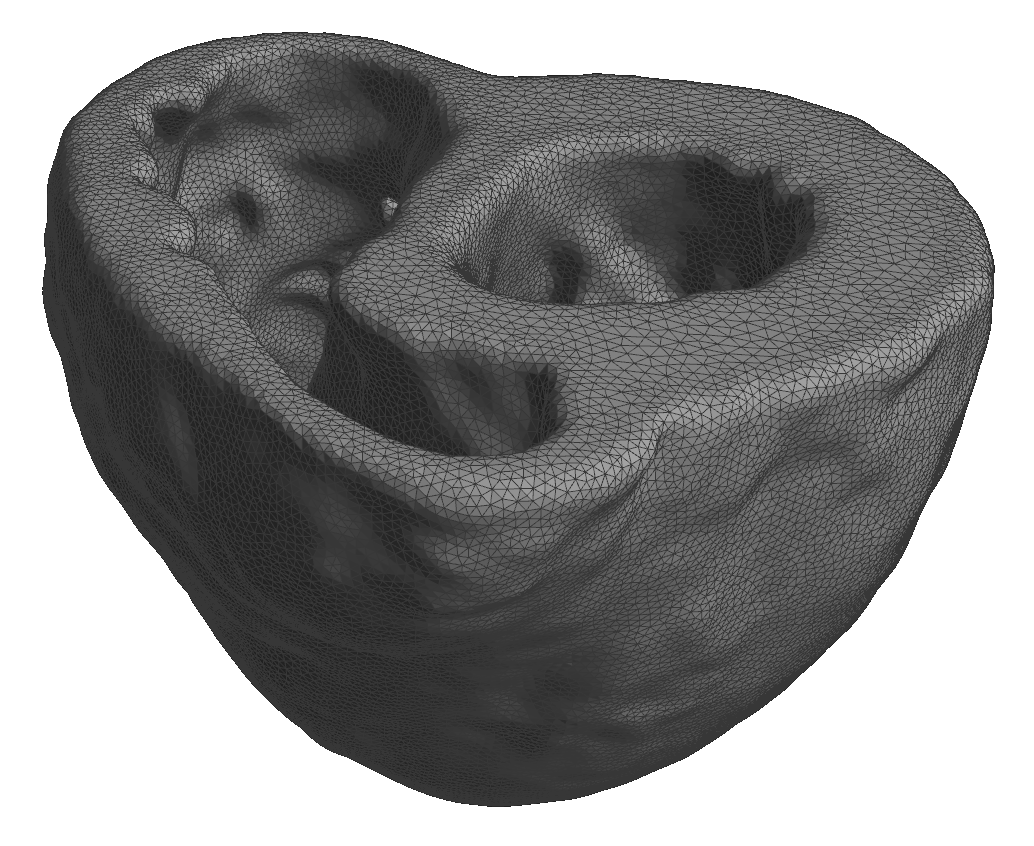
\includegraphics[scale=0.18]{media/3-celeris/1-brep.png}
\label{fig:cel1}}		
\subfigure[]{%
		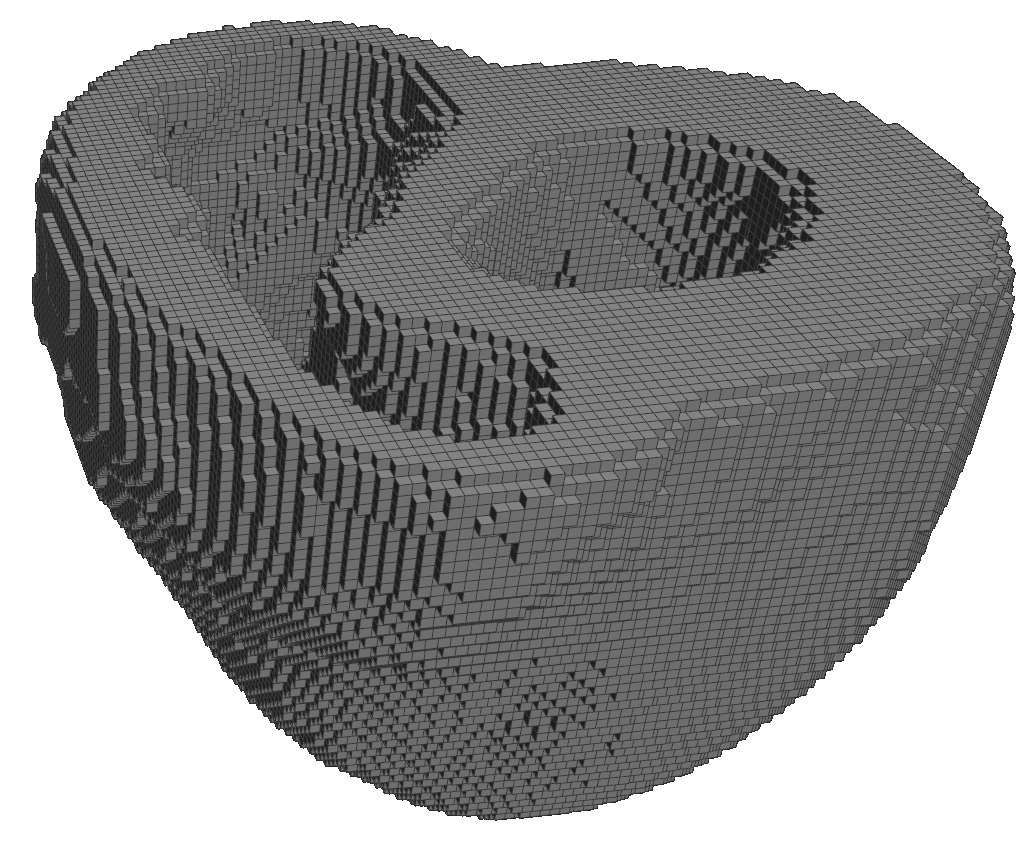
\includegraphics[scale=0.18]{media/3-celeris/2-hex.png}
\label{fig:cel2}}		
\subfigure[]{%
		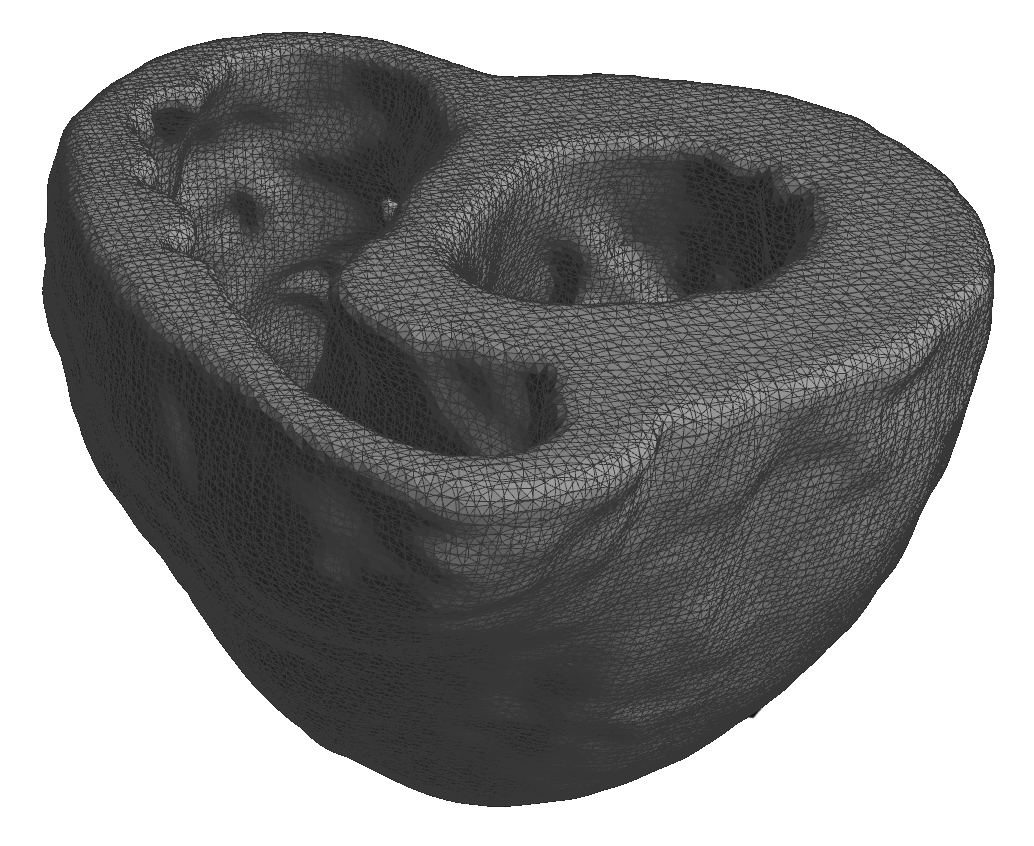
\includegraphics[scale=0.18]{media/3-celeris/3-pmesh.png}
\label{fig:cel3}}
\\		
\subfigure[]{%
		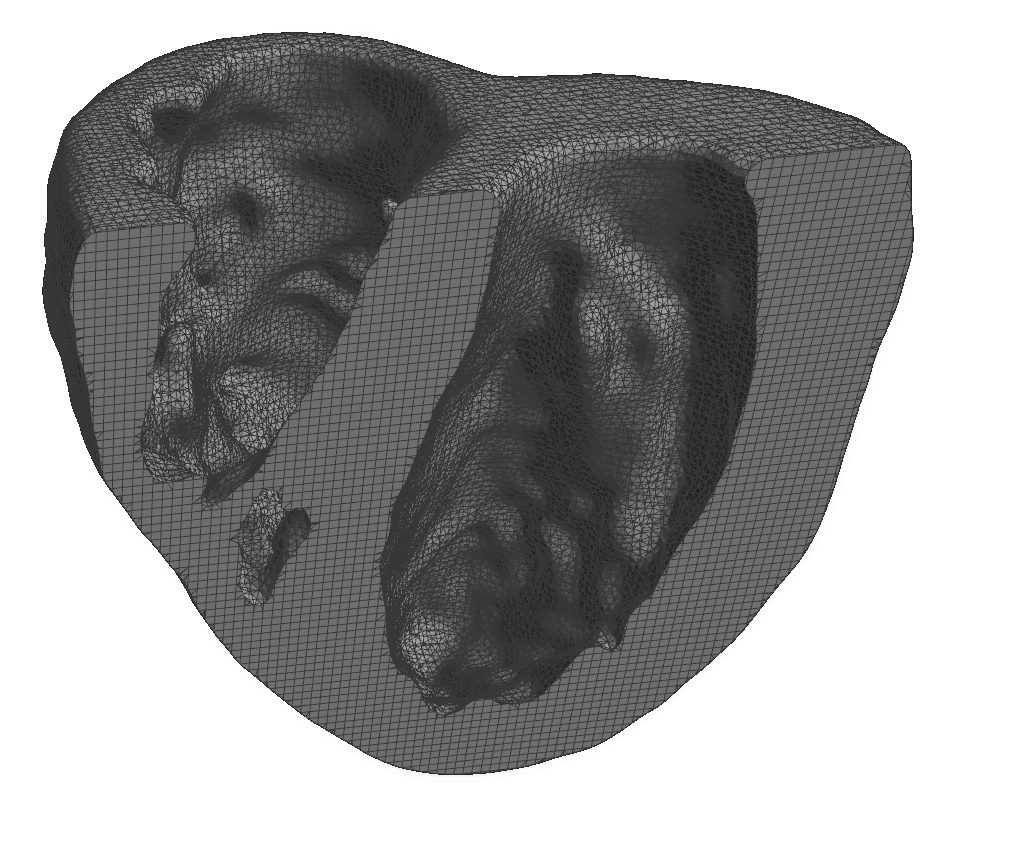
\includegraphics[scale=0.18]{media/3-celeris/4-clip.png}
\label{fig:cel4}}	
\subfigure[]{%
		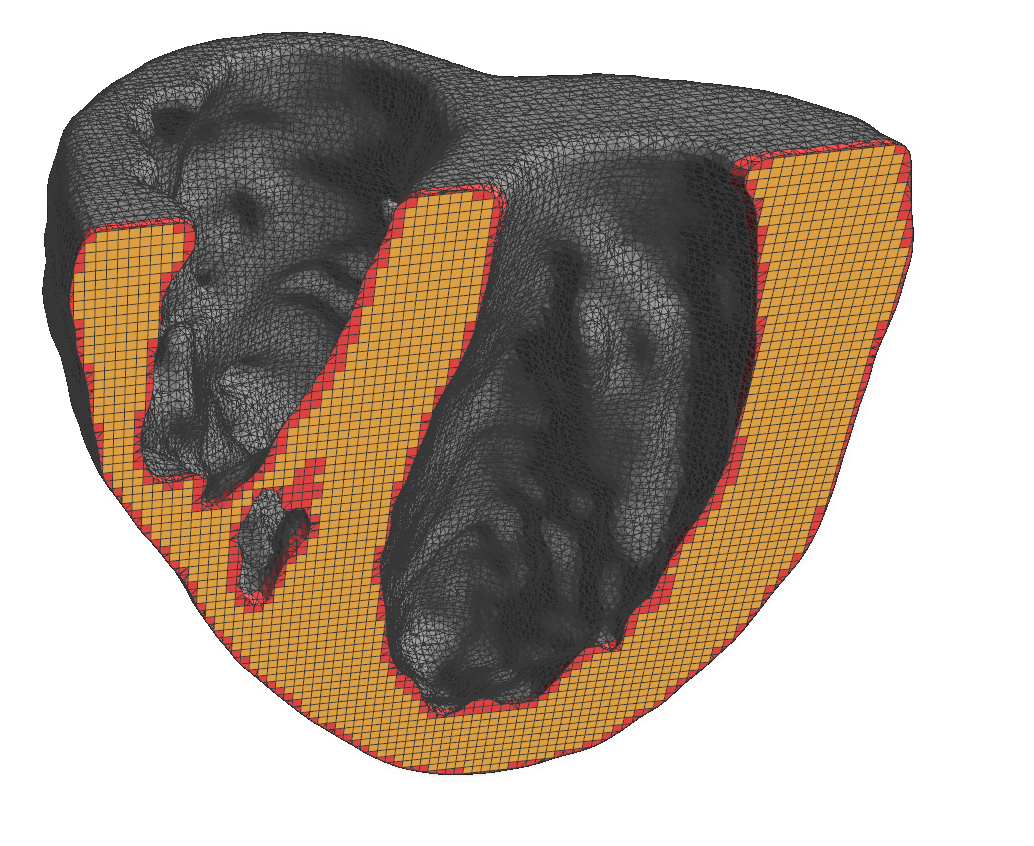
\includegraphics[scale=0.18]{media/3-celeris/5-color.png}
\label{fig:cel5}}			
\caption{Generation of polyhedral mesh: (a) input surface mesh, (b) bounding hex mesh,  (c) resulting polyhedral mesh, (d) clipped mesh, and (e) highlight of elements with cuboidal vs. general polyhedral shape}
\label{fig:cel}
\end{sidewaysfigure}

\begin{figure}[htbp!]
\centering
\subfigure[]{%
		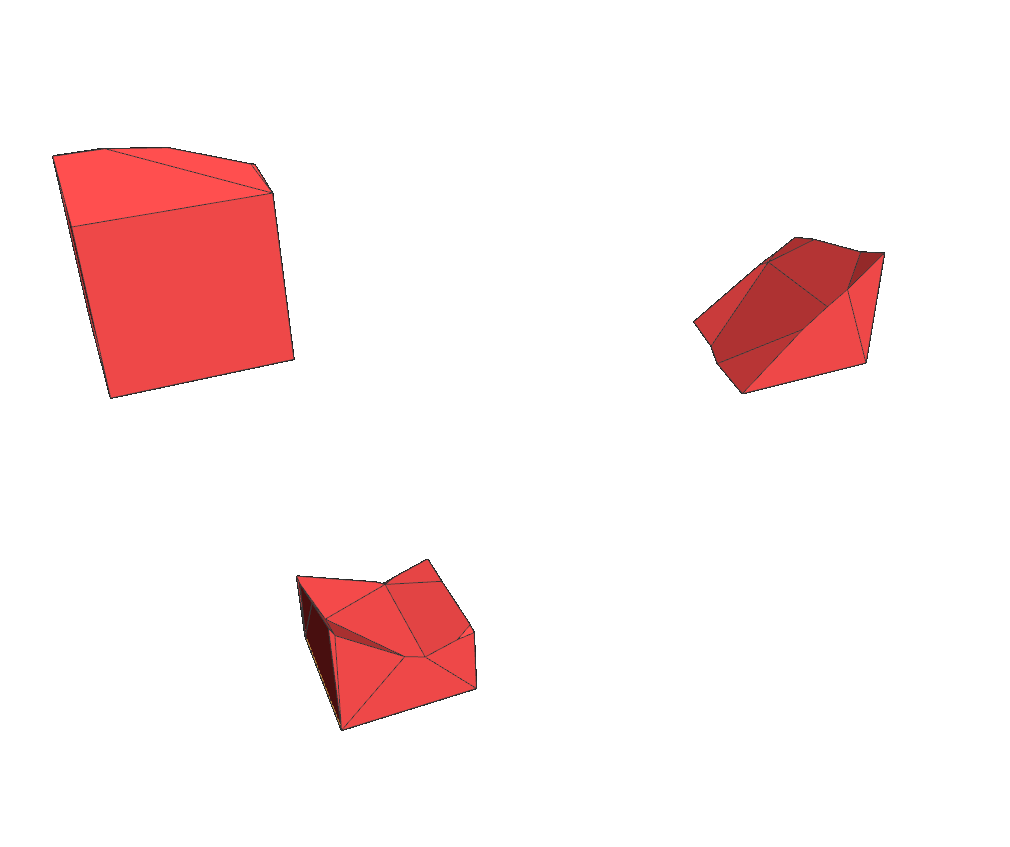
\includegraphics[scale=0.125]{media/3-celeris/zoom/zoom1.png}
\label{fig:zoom1}}		
\hfill
\subfigure[]{%
		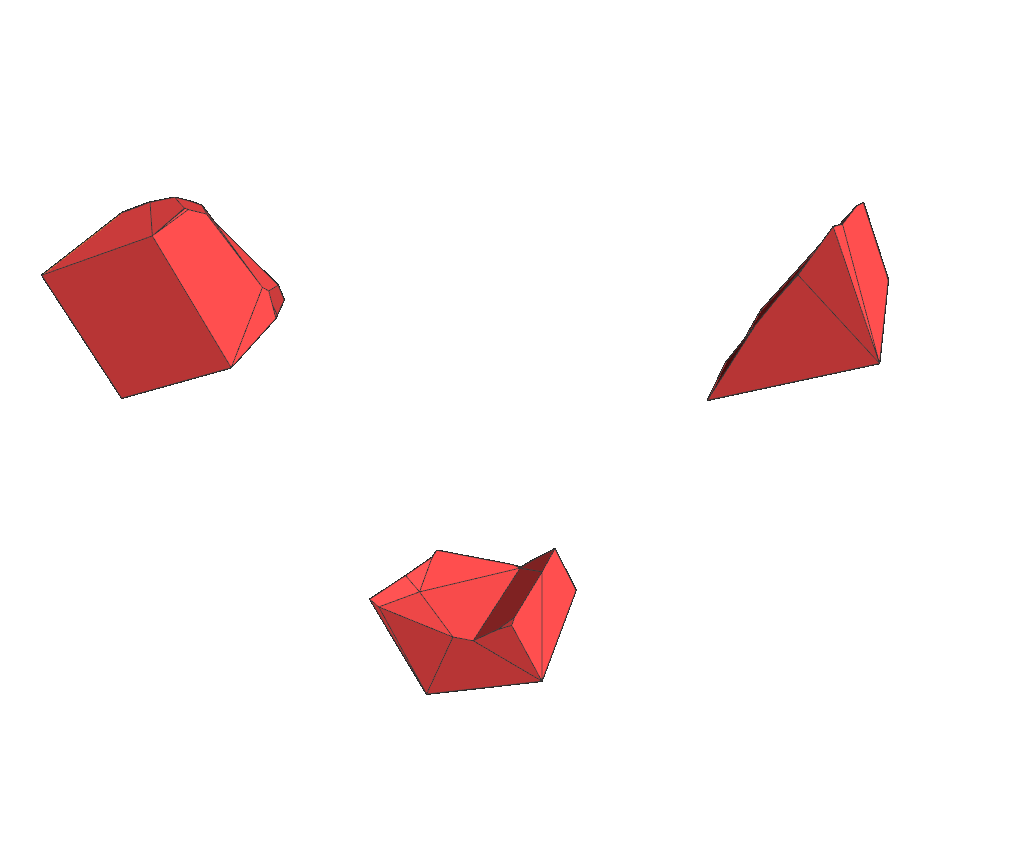
\includegraphics[scale=0.125]{media/3-celeris/zoom/zoom2.png}
\label{fig:zoom2}}		
\hfill
\subfigure[]{%
		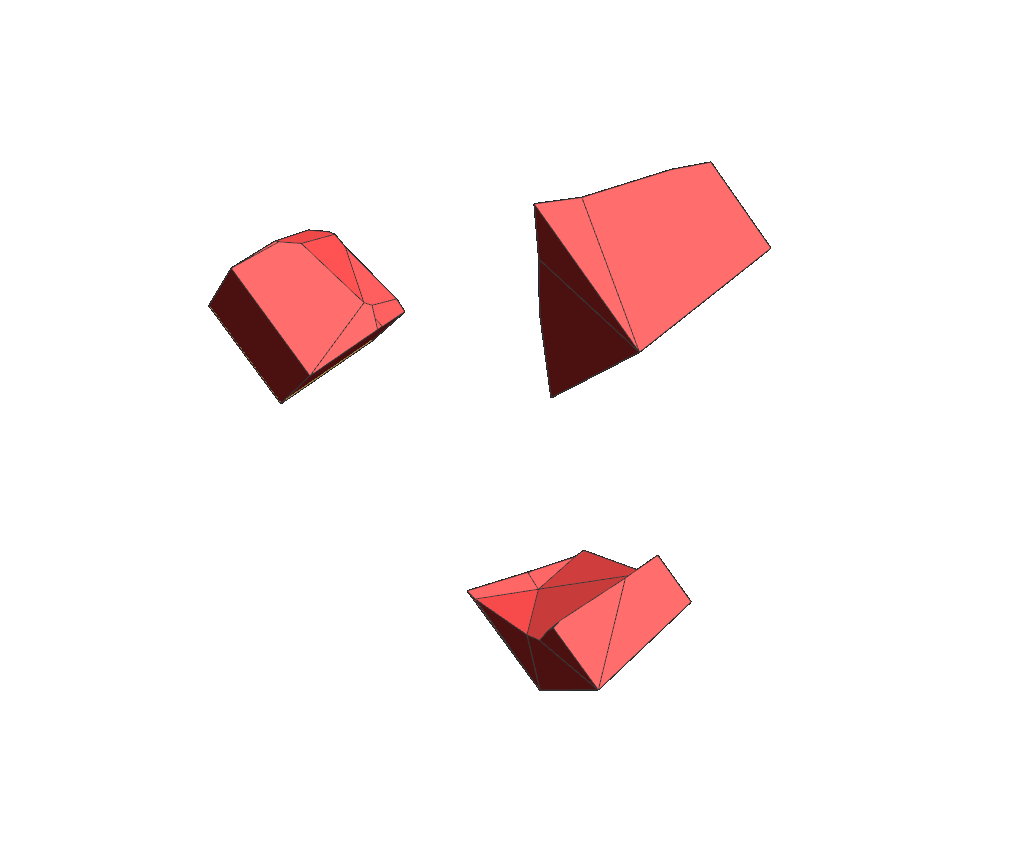
\includegraphics[scale=0.125]{media/3-celeris/zoom/zoom3.png}
\label{fig:zoom3}}		
\subfigure[]{%
		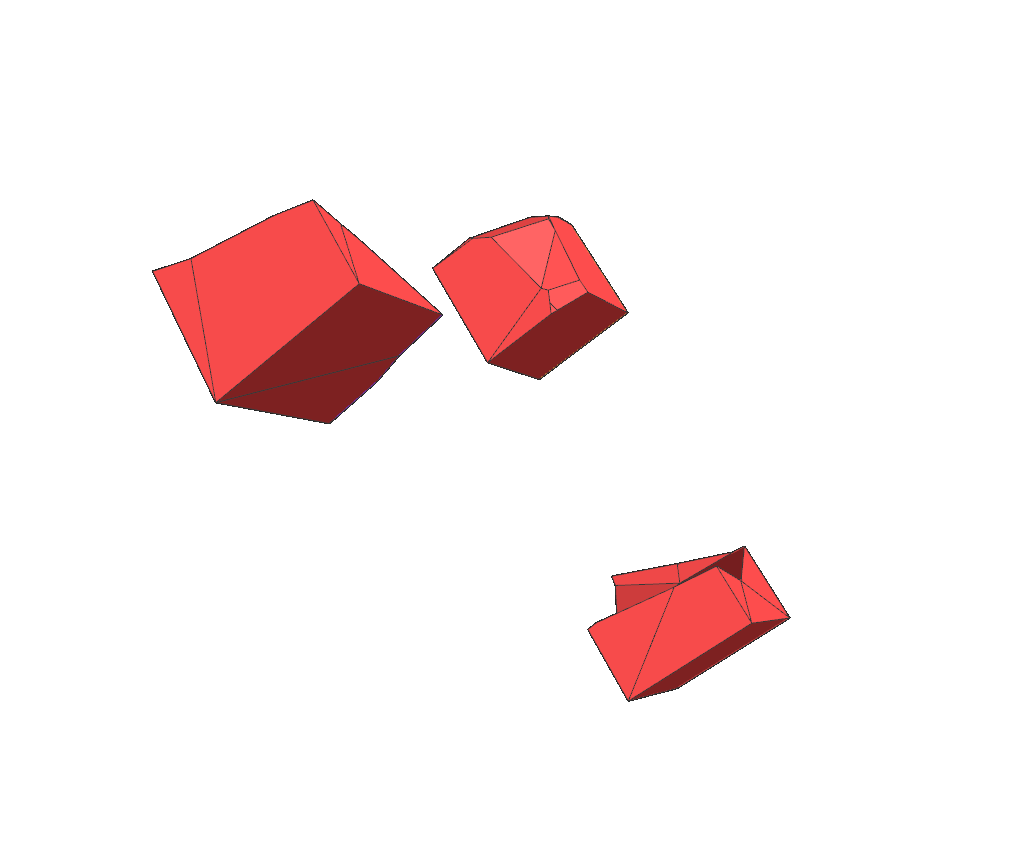
\includegraphics[scale=0.125]{media/3-celeris/zoom/zoom4.png}
\label{fig:zoom4}}	
\hfill
\subfigure[]{%
		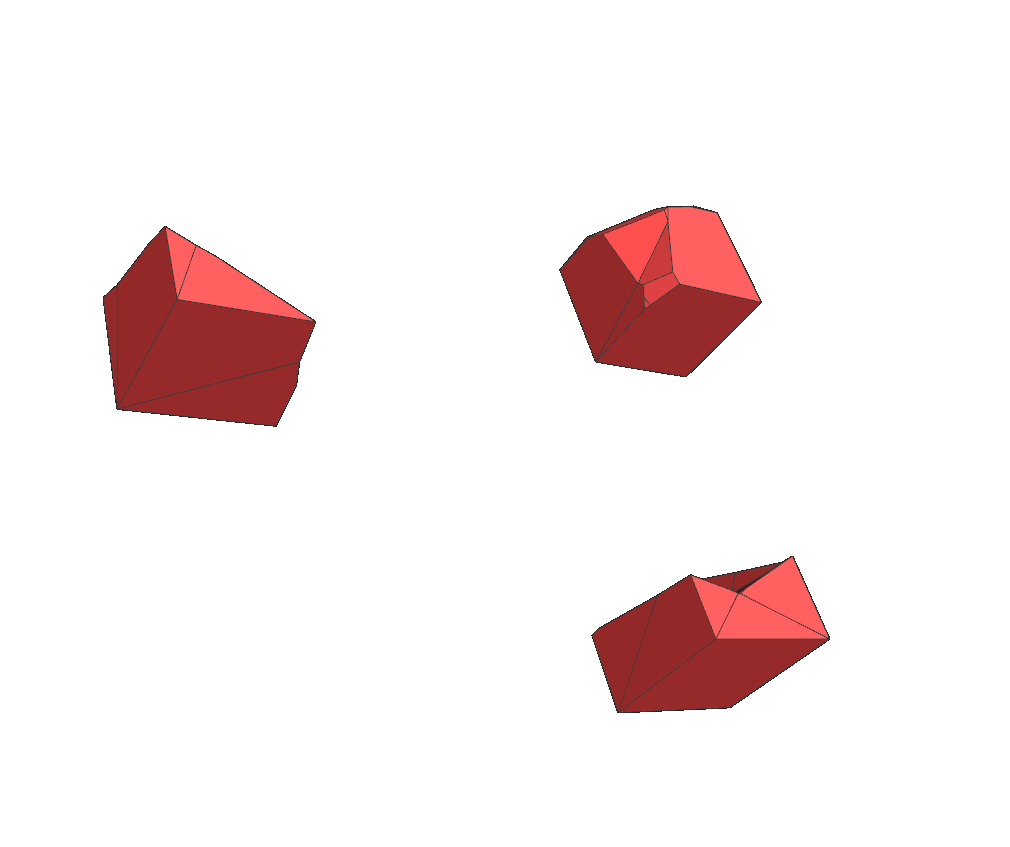
\includegraphics[scale=0.125]{media/3-celeris/zoom/zoom5.png}
\label{fig:zoom5}}		
\hfill
\subfigure[]{%
		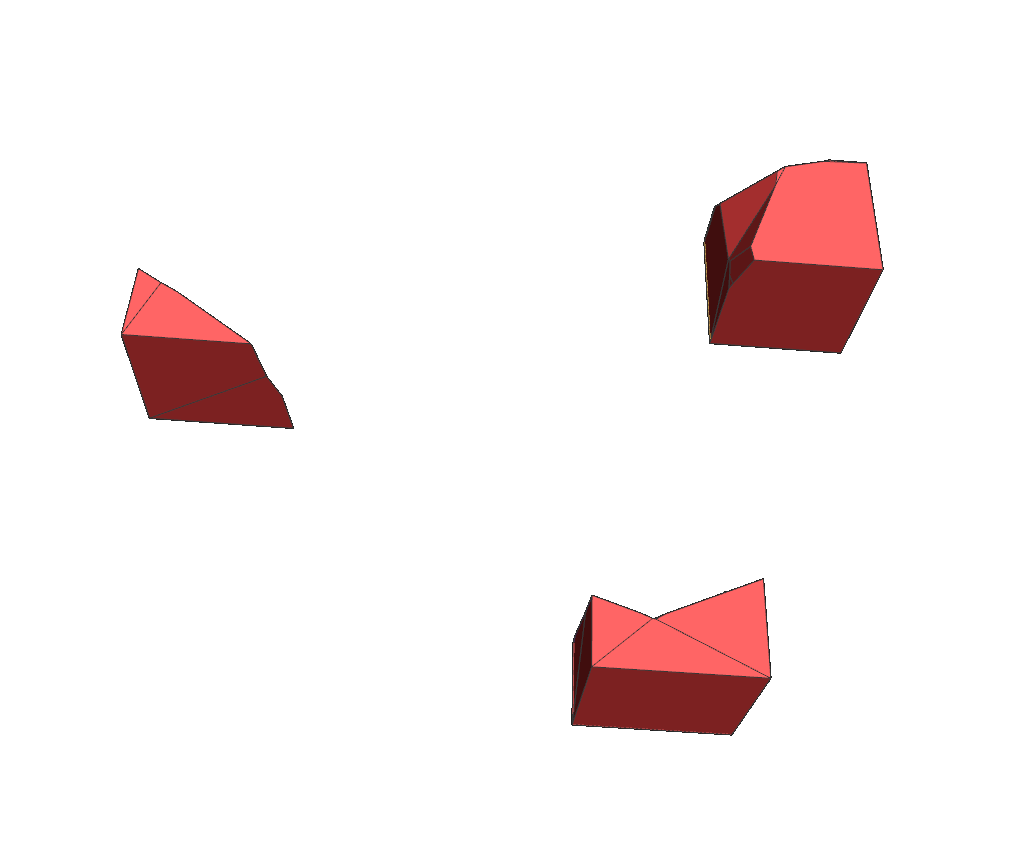
\includegraphics[scale=0.125]{media/3-celeris/zoom/zoom6.png}
\label{fig:zoom6}}	
\caption{Three example arbitrary polyhedral elements presented at different angles}
\label{fig:zoom}
\end{figure}

As it pertains to image-based modeling and simulation, the greatest benefit that polyhedral approaches offer is a separation between the \textit{simulation resolution} and the \textit{geometric resolution}. More detail will come in \chapref{4} regarding the polyhedral element formulation, but for this discussion the key is that nodal degrees of freedom are only defined at the points involving the background mesh, independent of the input b-rep. Thus, one can simultaneously retain a high fidelity description of a surface while performing a simulation at a significantly lower resolution. For the other meshing approaches described in this chapter, the volume mesh resolution is implicitly constrained by the input surface mesh resolution. For complex geometries found in biological tissues, the surface mesh resolution is almost always sacrificed to avoid an unwieldy number of degrees of freedom in the subsequent finite element solution.

For the same bi-ventricular surface mesh of the \textit{ex vivo} human heart example generated by the algorithm described in the previous section, volume meshes are compared between linear polyhedral elements and quadratic tetrahedral elements. Linear polyhedral elements are chosen for comparison because they behave and perform like linear hexahedra, and thus are sufficient for generating accurate solutions. The same surface mesh with desired resolution of 50k points and desired maximum element volume of 2 $mm^3$ is supplied to: the sculpt routine in Celeris; the Delaunay tetrahedralization routine in Tetgen; and the advancing front routine in Simpleware. ~\figref{compdof} shows that for this example, the polyhedral approach reduces the system size by a factor of 2 or more. The reduction in system size stems first from the fact that the polyhedral elements are lower order compared to the tetrahedral elements (87$\%$ of the 2.5 million DOF in the Simpleware mesh correspond to midside nodes), and second from not requiring an unnecessarily large number of surface \textit{nodes} to accommodate the large number of surface \textit{points}. It should be emphasized that even at this surface resolution, a noticeable degree of geometric features are sacrificed. The greater the importance of geometric fidelity, the greater the value the polyhedral approach offers in reducing the system size.

\begin{figure}[ht!]
\centering
		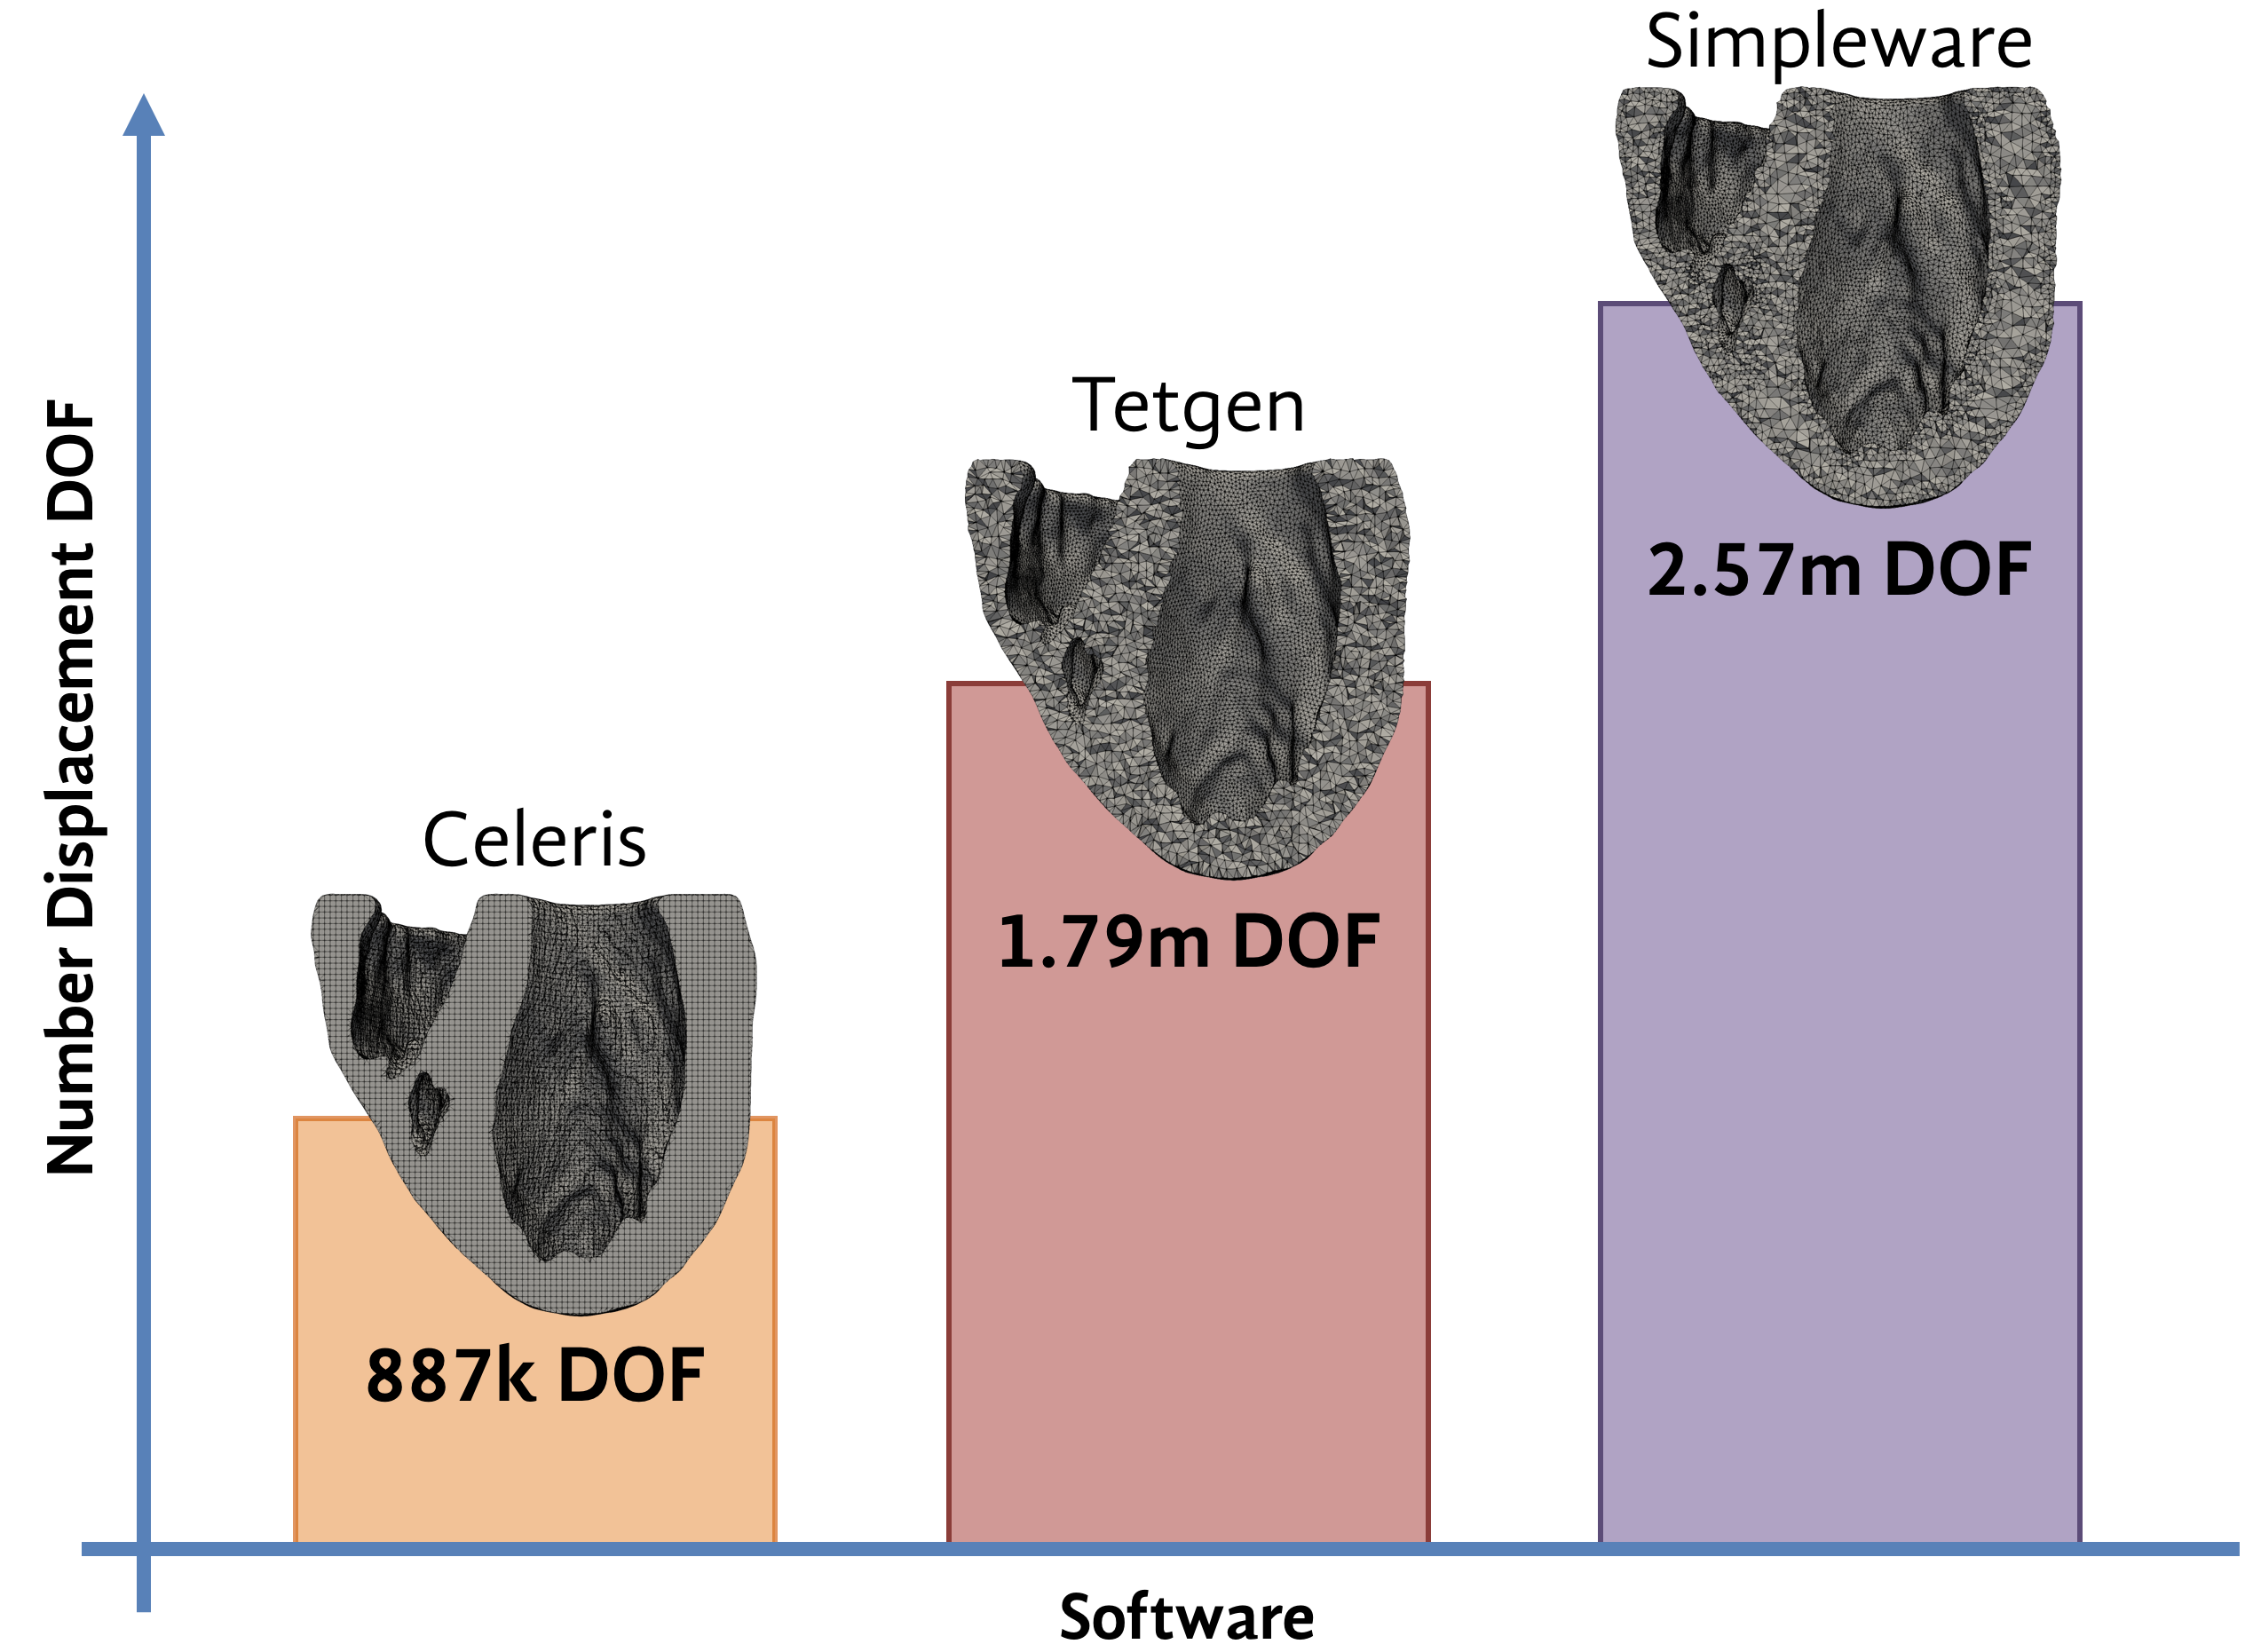
\includegraphics[scale=0.2]{media/comparison.png}
%\subfigure[]{%
%		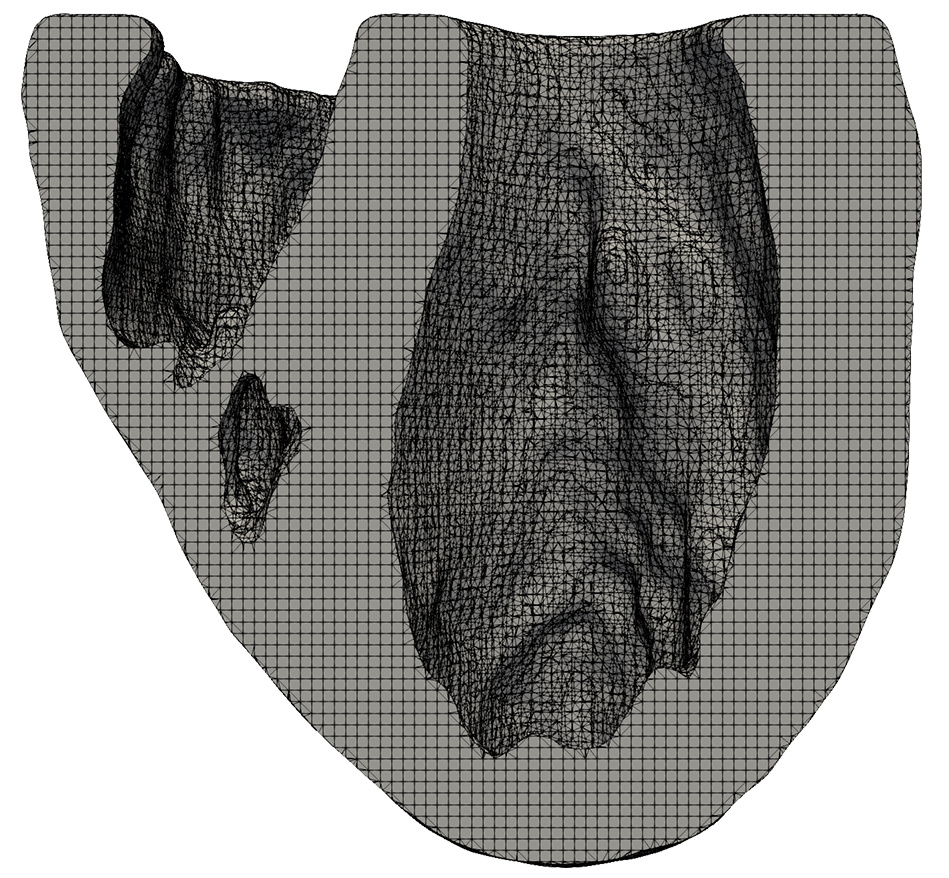
\includegraphics[scale=0.15]{media/3-celeris/8-celeris.png}
%\label{fig:comp-1}}		
%\subfigure[]{%
%		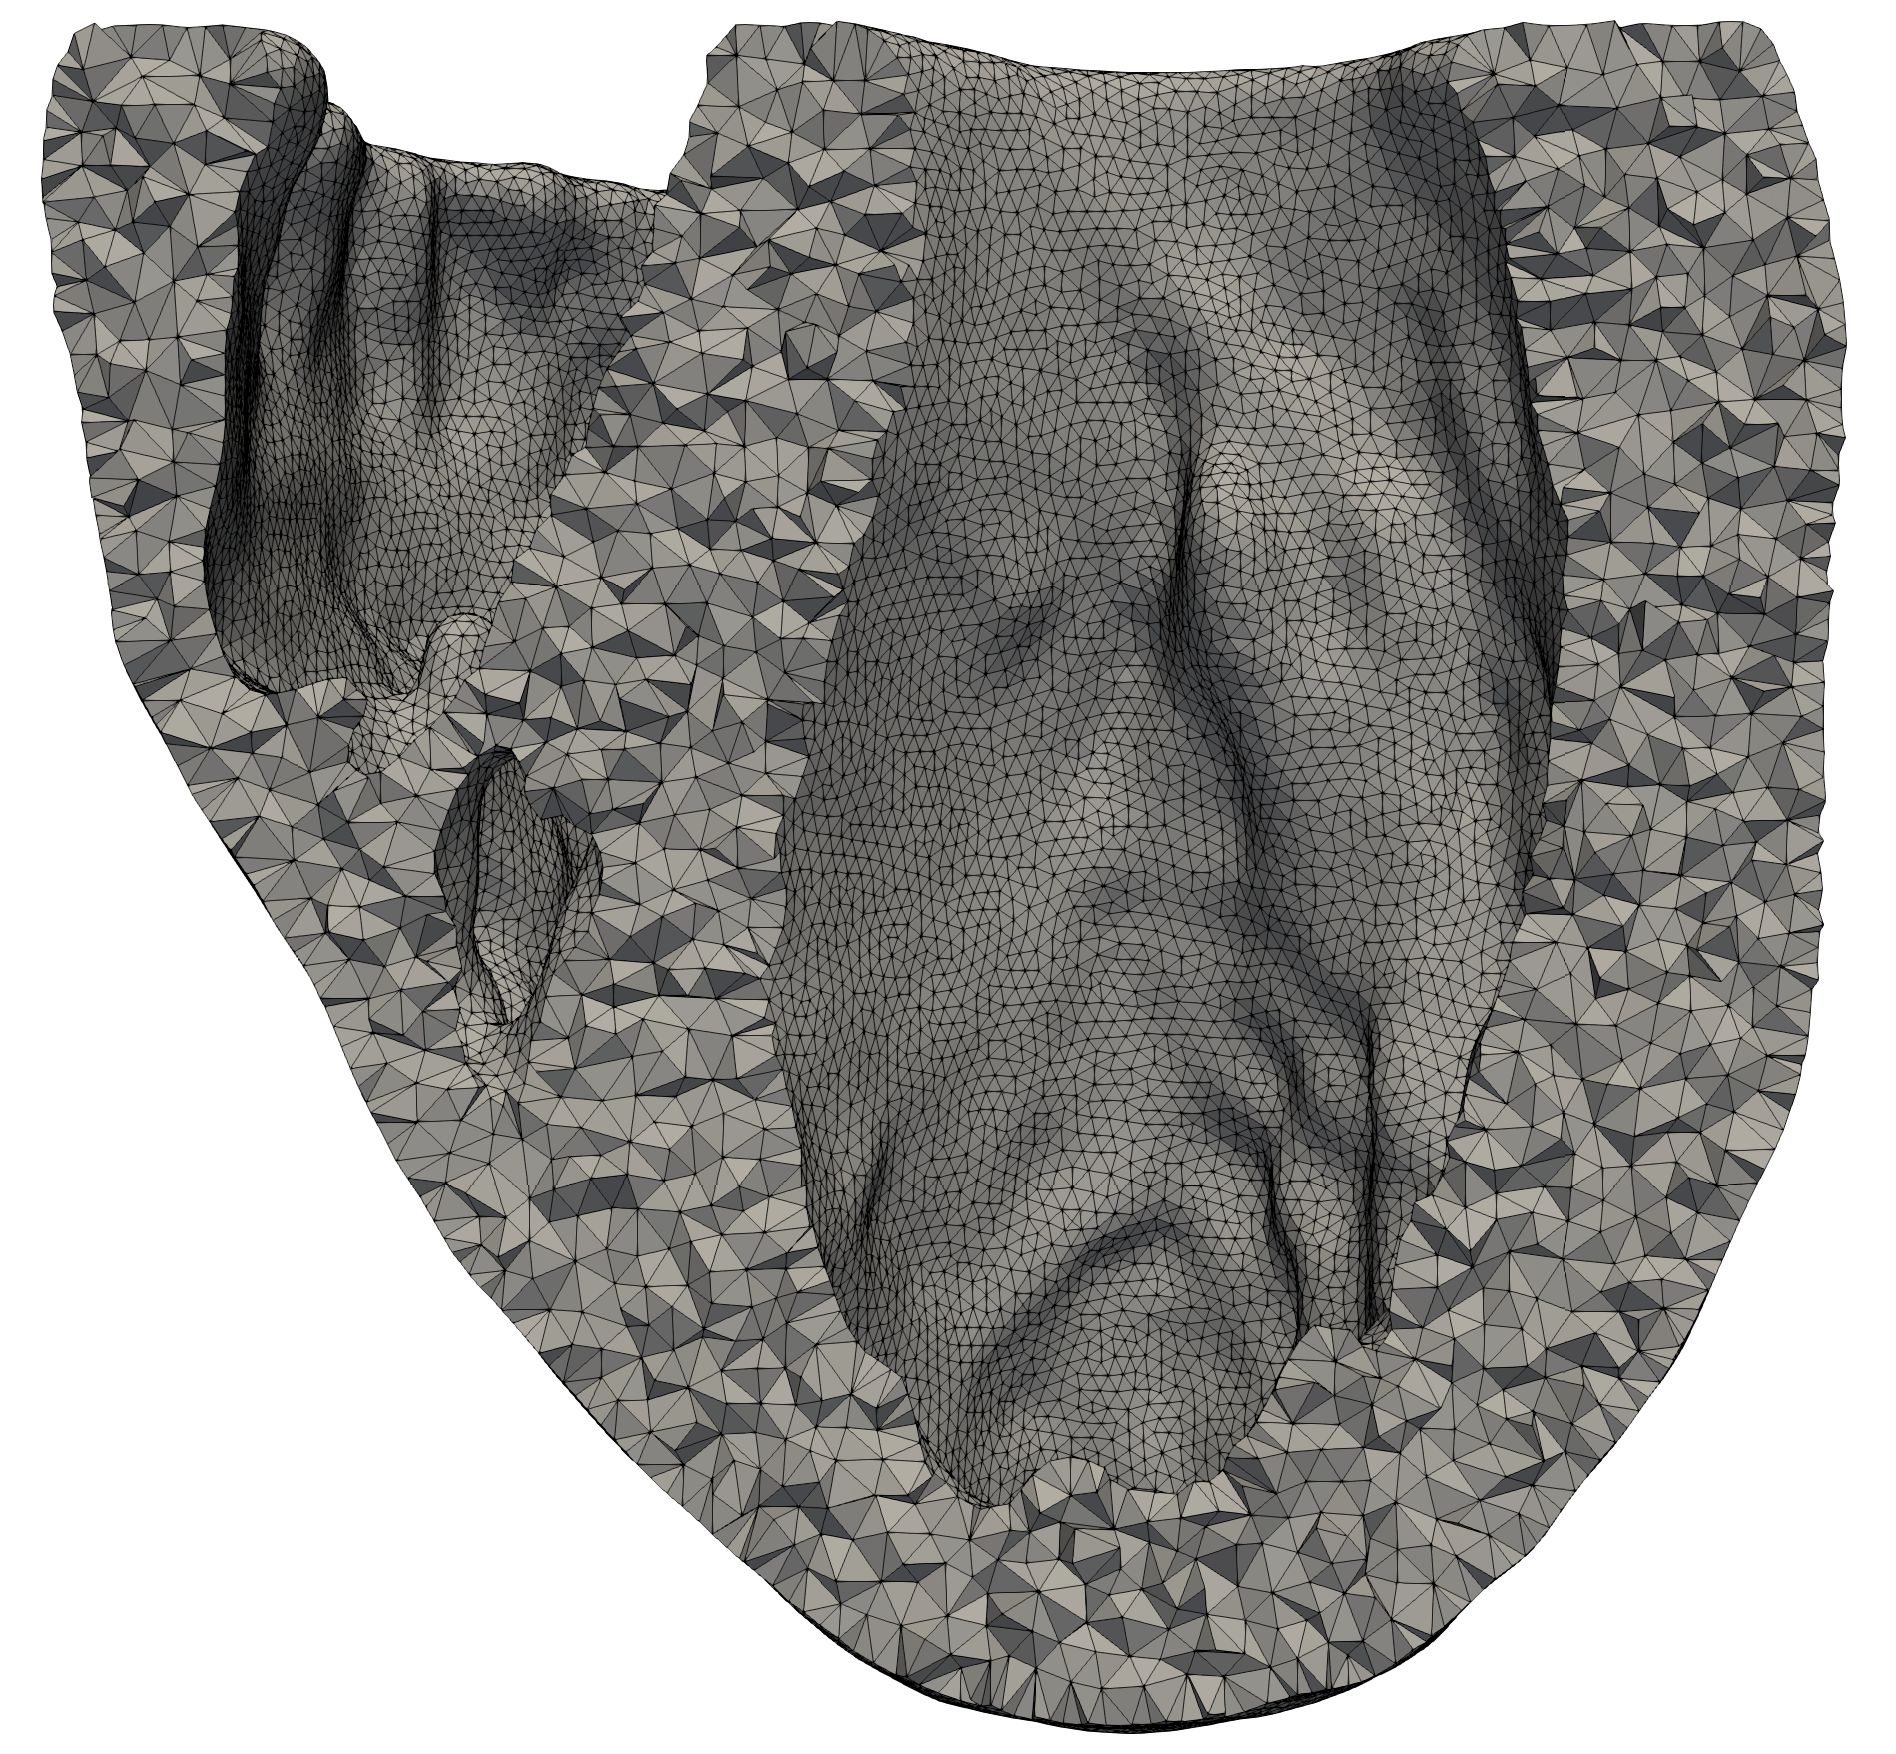
\includegraphics[scale=0.15]{media/3-celeris/9-cardioid.png}		
%\label{fig:comp-2}}	
%\subfigure[]{%
%		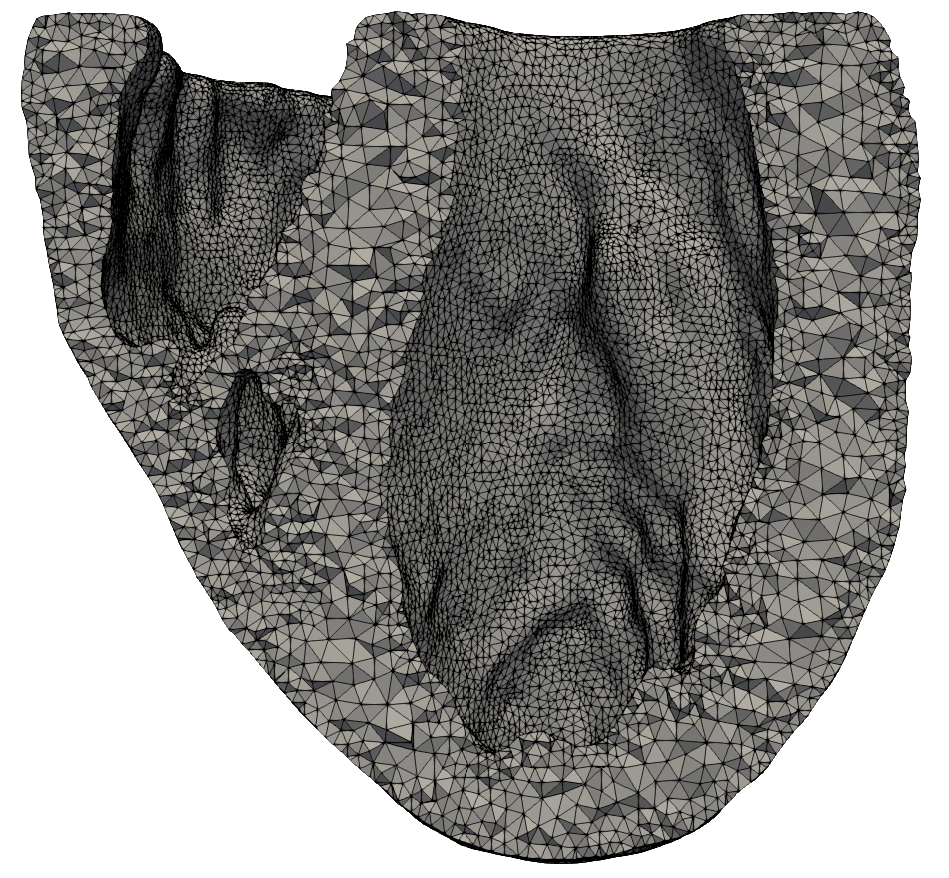
\includegraphics[scale=0.15]{media/3-celeris/10-simpleware.png}
%\label{fig:comp-3}}				
%
\caption{Comparison of meshes between: linear polyhedral mesh from Celeris; quadratic tetrahedral mesh from Tetgen; and quadratic tetrahedral mesh from Simpleware. Note, Simpleware focuses on generating high quality elements, hence the larger number of DOF compared to Tetgen.}
\label{fig:compdof}
\end{figure}

The final result of the workflow from image to image mask to b-rep to polyhedral mesh is demonstrated in ~\figref{celsuite} for \textit{ex vivo} canine and human heart ventricles from the CardioVascular Research Grid~\cite{cvgg}.

\begin{sidewaysfigure}[htbp!]
\centering
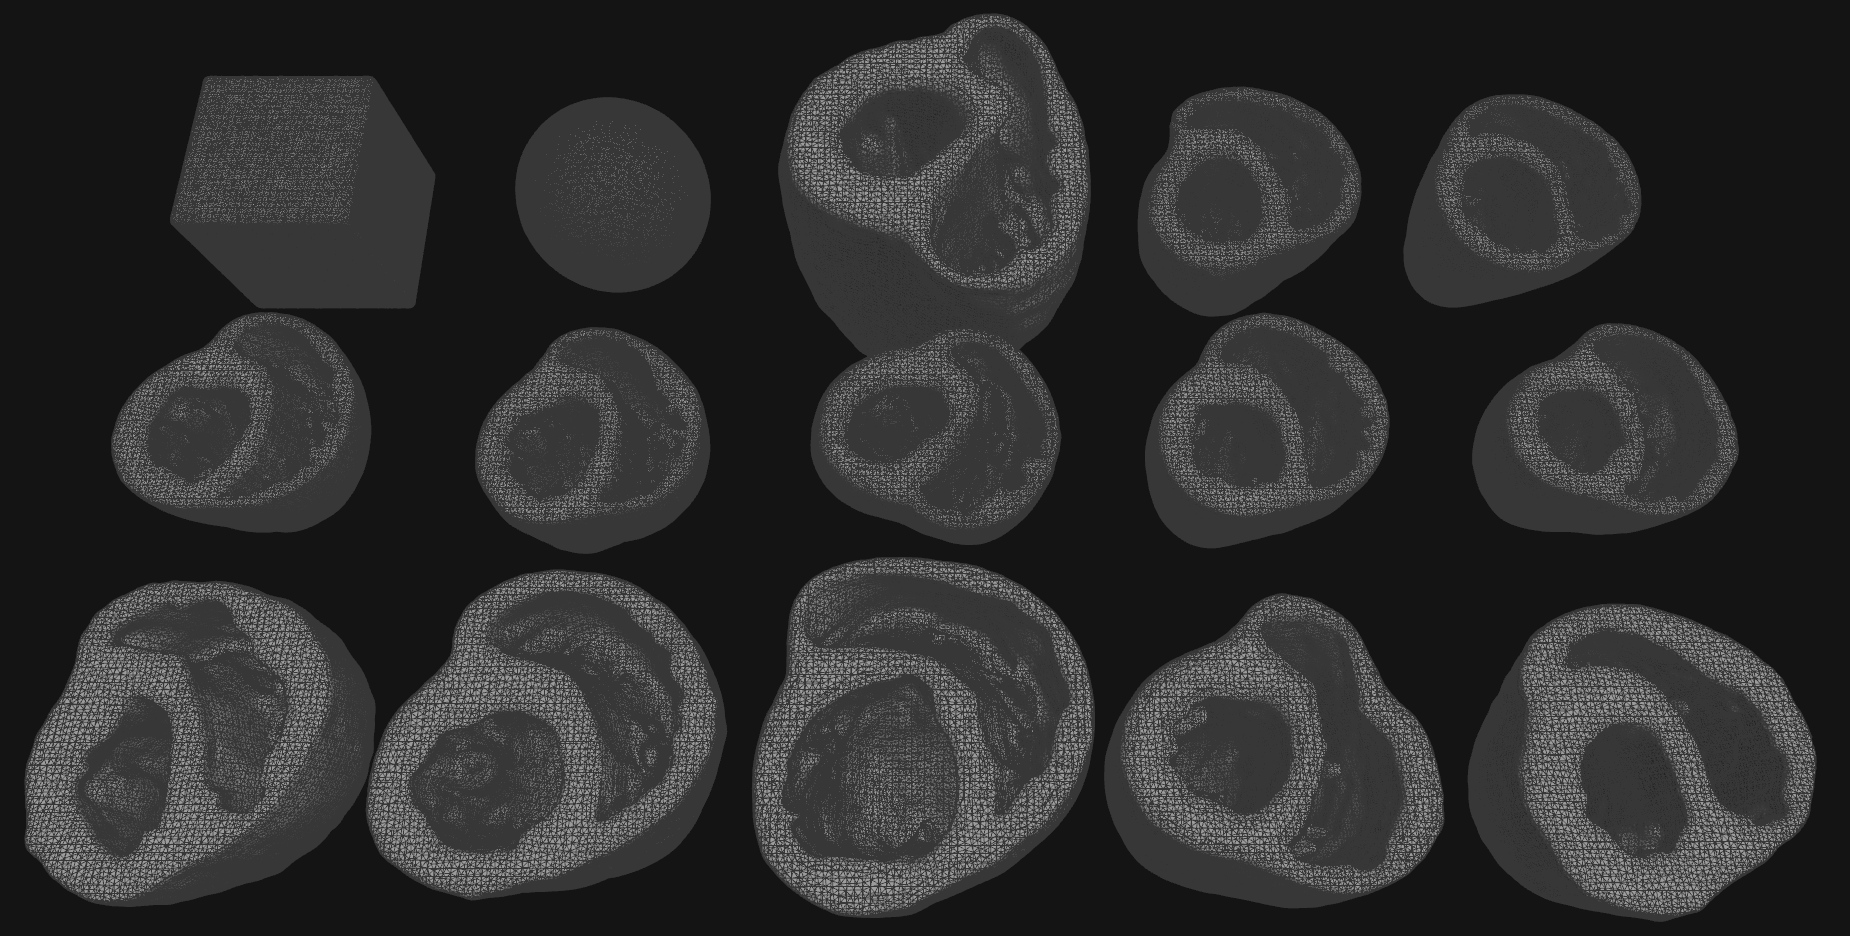
\includegraphics[width=1.0\textwidth]{media/3-celeris/7-suite.png}
\caption{Suite of polyhedral finite element meshes generated from image data \vspace{1cm}}
\label{fig:celsuite}
\end{sidewaysfigure}

%%%%%%%%%%%%%%%%%%%%%%%%%%%%%%%%%%%%%%%%%%%%%%%
%%%%%%%%%%%%%%%%%%%%%%%%%%%%%%%%%%%%%%%%%%%%%%%
\subsection{File Formats}
\label{File Formats-MESH}
File formats for volume meshes follow the same paradigm as for point clouds and surface meshes. Namely, spatial coordinates of points are listed, followed by a list of elements that are defined based on connectivities of those points. The tetrahedral meshes generated by Tetgen are stored in VTK format or \textit{Abaqus} INP~\cite{abaqus} format. Polyhedral meshes are stored in a similar manner, but each element additionally requires a listing of facet data to accommodate arbitrary polyhedral topology. For the purposes of running simulations, additional information may be included with the mesh, such as surface sets or point sets for the purposes of assigning boundary conditions.

\section{Shabaka: A Free Image-Based Meshing Tool}

The image-based meshing steps described in this chapter are assembled to form a novel image-based meshing tool \textit{Shabaka}~\cite{shab}, available on GitHub at~\href{http://github.com/omhafez/shabaka}{{\url{http://github.com/omhafez/shabaka}}}. A screenshot of the repository on GitHub is shown in~\figref{github}.

\begin{figure}[ht!]
\centering
\vspace{2.5mm}
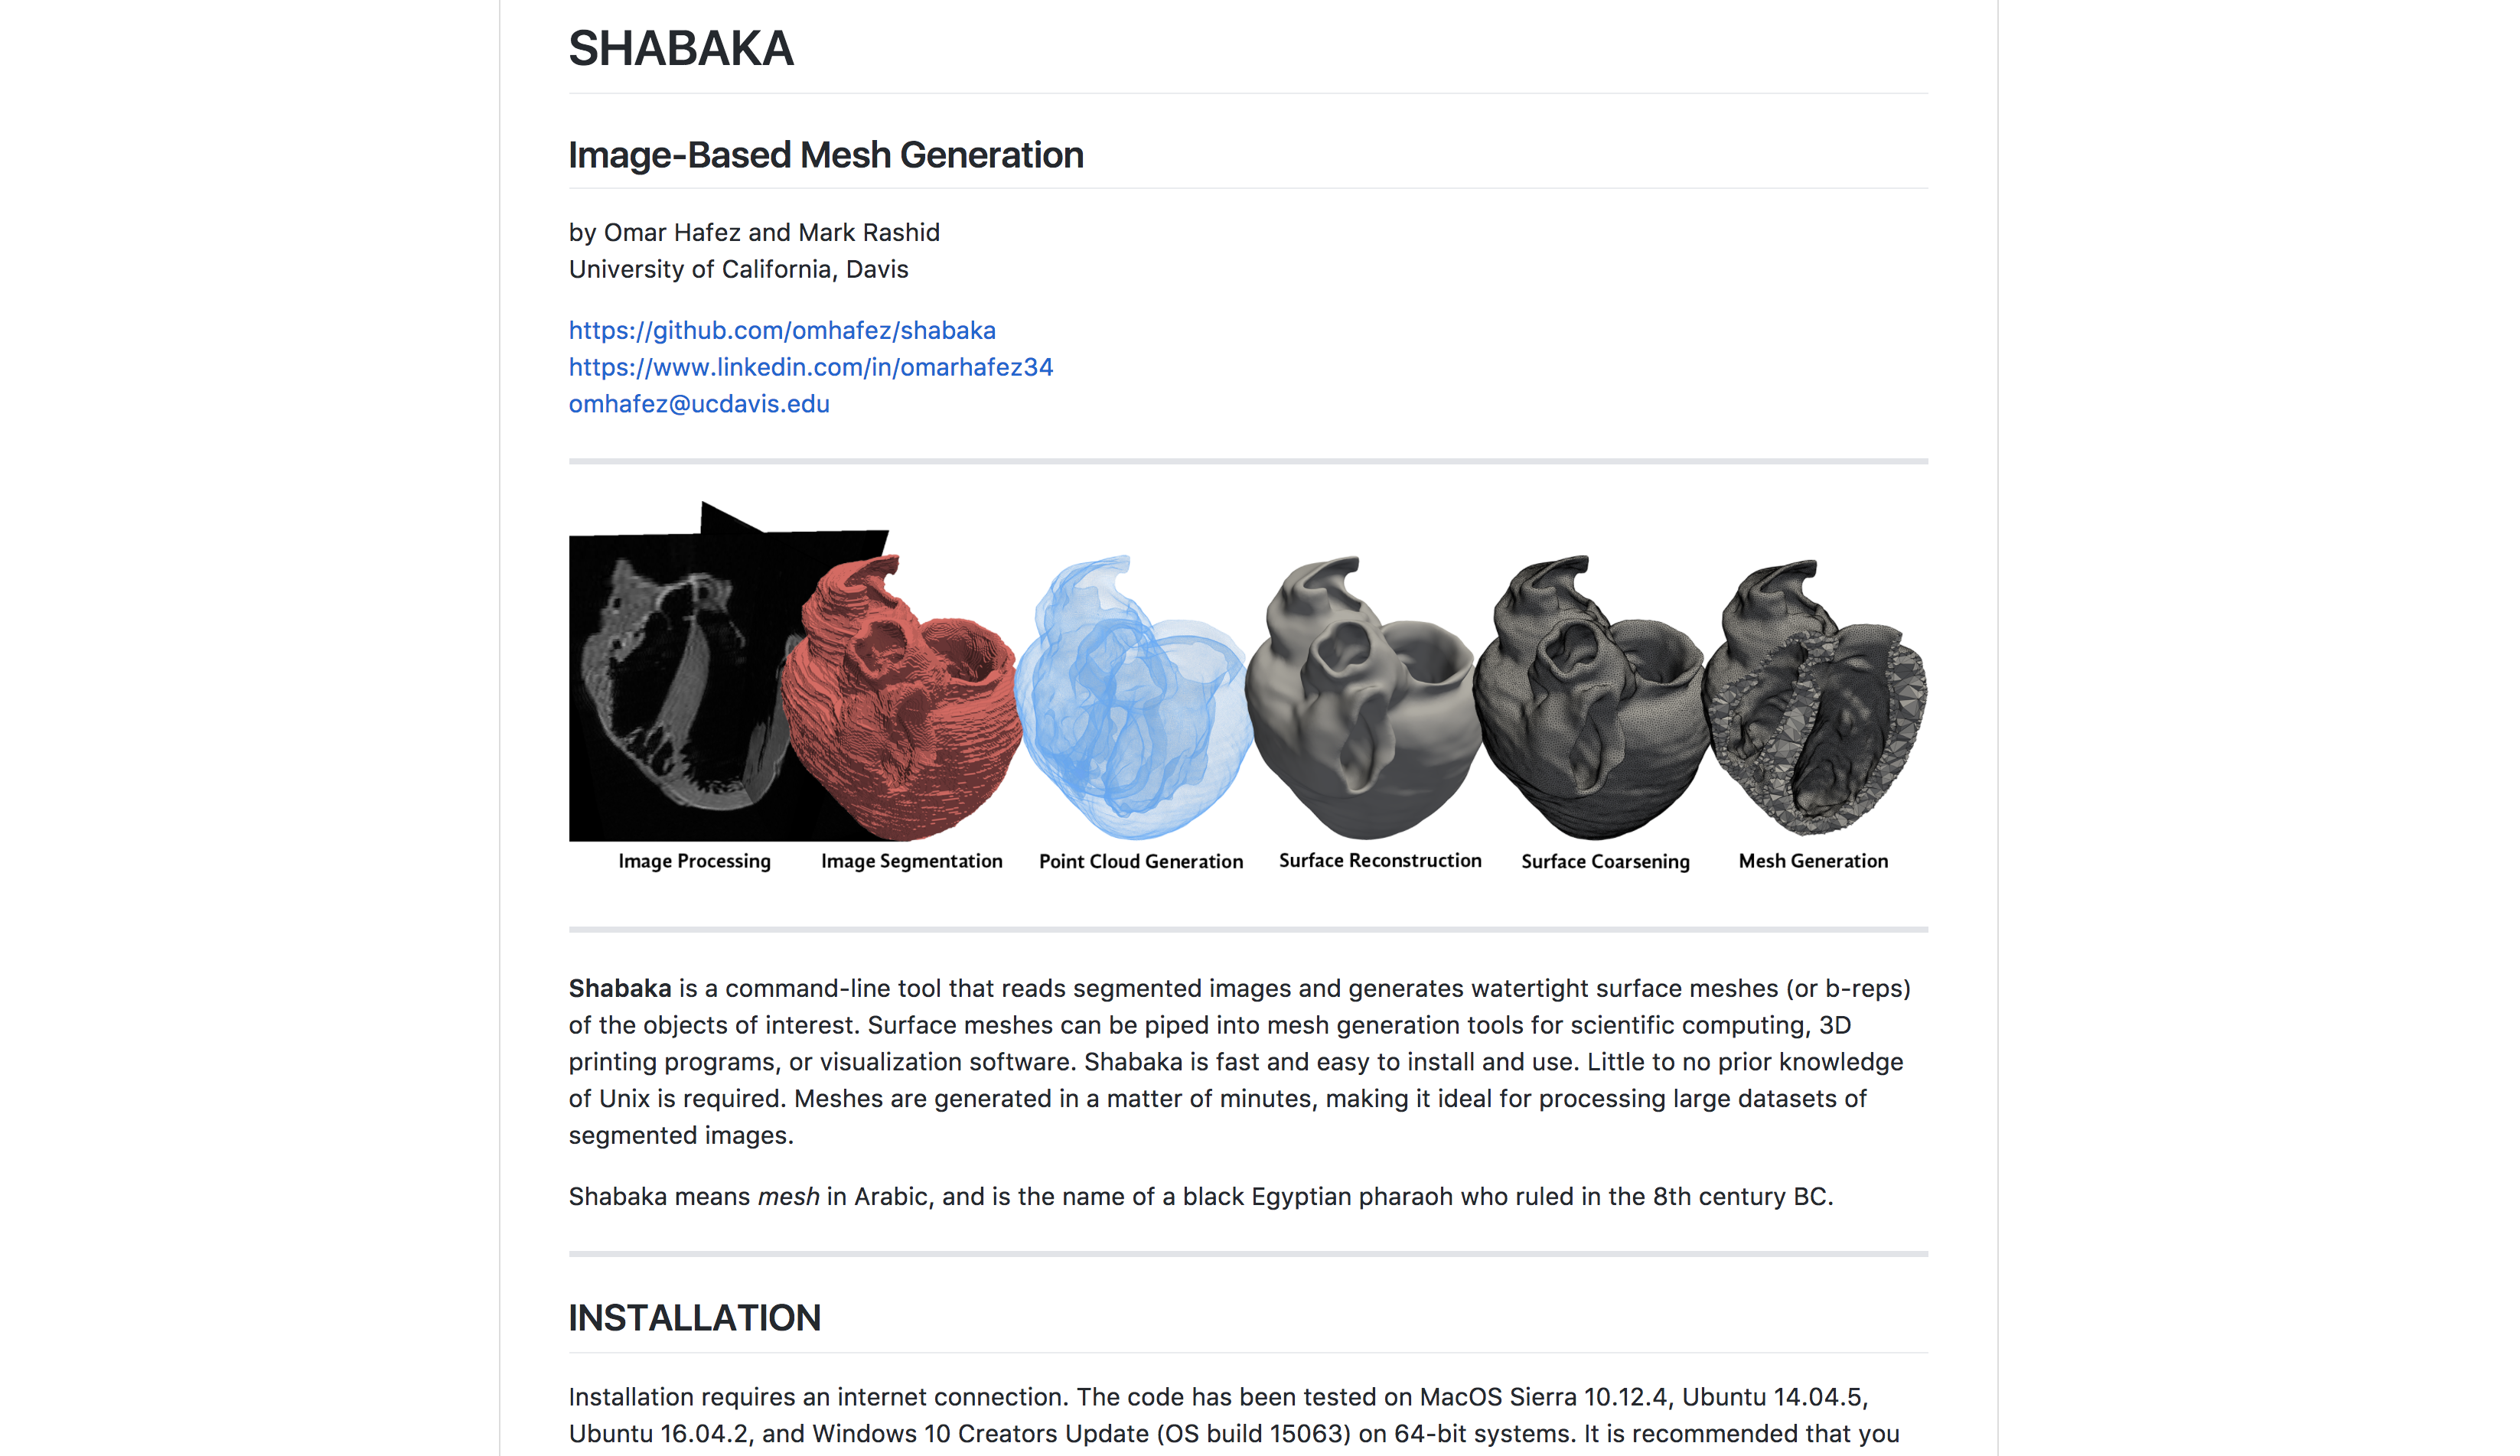
\includegraphics[width=1.0\textwidth]{media/2-shabaka/2-surf/7-shabaka.png}
\caption{Screenshot of Github repo}
\label{fig:github}
\end{figure}

Simple instructions are available to install the code on Linux, Mac, or Windows in about 15 minutes. A bash script compiles the code and downloads library dependencies including: \textit{NRRD}~\cite{nrrd} for image mask I/O, \textit{NLopt}~\cite{nlo} for nonlinear optimization, \textit{Qhull}~\cite{barber_1996} for Voronoi partitioning, \textit{ACVD}~\cite{valette_2004} for surface decimation, and \textit{Meshlab}~\cite{meshlab} and \textit{Gmsh}~\cite{geuzaine_2009} for miscellaneous mesh tasks. Libraries are gathered from the standard APT package manager on Ubuntu and from \textit{Homebrew}~\cite{brew} on Mac. The Windows installation makes use of the \textit{Windows Subsystem for Linux (WSL)}, so installation is treated in the same manner as for Ubuntu. Unit tests are available to verify a successful installation and the utility of various components of the code.

Additional free software packages are included in the build to provide an end-to-end image-based meshing pipeline. Namely, \textit{Seg3D}~\cite{Seg3D} is included for image processing and image segmentation functionality, \textit{Tetgen}~\cite{tetgen} for tetrahedral meshing, and \textit{ParaView}~\cite{paraview} for visualization. Following a full installation of the code, the user can: process and segment a medical image in Seg3D to produce an image mask; produce a high quality surface mesh with Shabaka; produce a tetrahedral mesh using Tetgen; and visualize the resulting mesh in ParaView. Documentation on how to efficiently segment images in Seg3D has been written and included in the GitHub repo, along with essential publications related to steps in the workflow. The tool is catered toward users of simulation, 3D printing, or visualization software. No prior knowledge or understanding of image segmentation, mesh generation, or UNIX is required.

The core code for Shabaka is written in C++ and Fortran, along with Python scripts to facilitate the interaction between different portions of the code with external packages. After processing command-line inputs, the code reads the input image mask in NRRD format. The code automatically resamples segmented images that do not exhibit isotropic voxel spacing. In this manner, the point cloud generation step may assume every input image mask has equal spacing in all three directions. The point cloud generation code in C++ is easily parallelized since interfaces are approximated for each window independently of one another. The final oriented point cloud is exported in PLY format. Voronoi site locations are generated and provided to the Voronoi partitioning tool. The surface mesh is subsequently extracted, cleaned, and decimated. The final surface is exported in both PLY and STL formats.

The code has a simple UNIX environment interface that offers a number of command-line options. Options include the ability to specify a desired mesh resolution, and whether to automatically call Tetgen to produce a tetrahedral mesh from the surface generated from Shabaka. The option is also available to call the Meshlab implementation of screened Poisson surface reconstruction as an alternative to the default Voronoi-based surface reconstruction technique. Resulting surface meshes from screened Poisson surface reconstruction tend to be over-smoothed compared to those from the Voronoi-based approach. The implementation in Meshlab performs impressively fast, though, and tends to be more robust for particularly challenging surfaces, where in rare cases Voronoi approach fails to produce a valid surface.

Shabaka is currently limited to meshing binary image masks. It can mesh multiple disjoint objects in a single image, but cannot currently produce meshes from multi-label masks. Each surface is watertight and manifold, and no manual correction of the mesh is required. A surface produced from Shabaka may be used as input to any software that accepts a surface mesh as input. As it pertains to the focus of this discussion, the surface mesh is inserted into a mesh generation tool, be it Tetgen for creating a quadratic tetrahedral mesh, or Celeris for creating a linear polyhedral mesh. The surface generation step typically takes less than 5 minutes for realistic input image masks using a 2.4 GHz Intel Core i7 processor with 16 GB RAM. In all, if the user has an image mask readily available, he or she can install Shabaka and generate a high quality surface mesh and subsequent volume mesh in less than half an hour on a typical laptop.

Shabaka has been rigorously tested against a wide variety of input images. Image masks have been meshed for the heart, brain, lungs, liver, skull, pelvis, vertebra, femur, and portions of the knee joint (see \figref{showcase}).

\begin{sidewaysfigure}[htbp!]
\centering
\vspace{2.5mm}
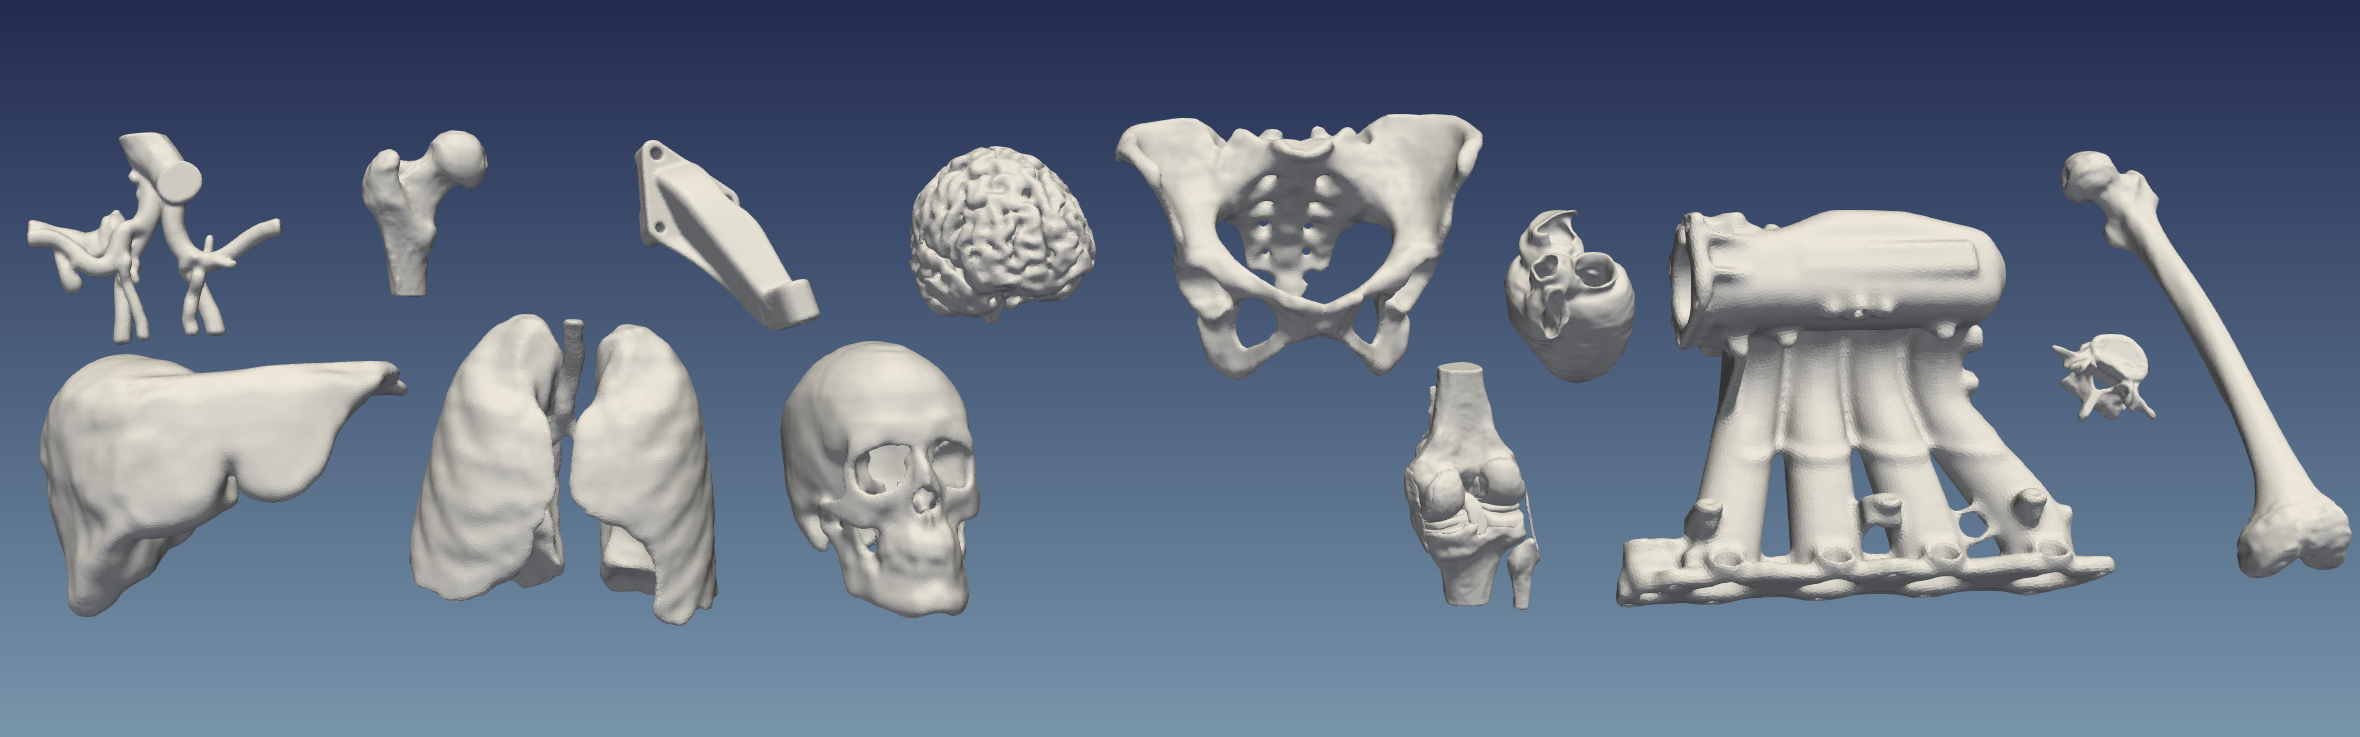
\includegraphics[width=1.0\textwidth]{media/2-shabaka/2-surf/6-showcase.png}
\caption{Suite of example meshes generated from image data using Shabaka}
\label{fig:showcase}
\end{sidewaysfigure}
